% ---------------------------------------------------------------------------- %
% file: disseration.tex
% author: Michael Pilosov
%
% LaTeX based on work by Sarah Kreidler and Peter DeWitt
% (github.com/dewittpe/ucd-dissertation-template)
%
%
% ---------------------------------------------------------------------------- %

\documentclass[english,10pt]{ucdenver-dissertation}
%%%%%%%%%%%%%%%%%%%%%%%%%%%%%%%%%%%%%%%%%%%%%%%%%%%%%%%%%%%%%%%%%%%%%%%%%%%%%%%%
% usepackages.tex

% ----------------------------------------------------------------------------- %
% a list of packages I commonly use in my LaTeX deliverables.
\usepackage[T1]{fontenc}
\usepackage[utf8]{inputenc}
\usepackage{textcomp}
\usepackage{floatrow}
\usepackage{url}
\usepackage{paralist}
\usepackage{xparse}
% \usepackage{enumitem}
\usepackage[ruled, vlined]{env/algorithm2e}
% source: https://ctan.org/tex-archive/macros/latex/contrib/algorithm2e/tex

%% Using ragged2e package to get left-justified, ragged-right text throughout body (JH)
\usepackage[document]{ragged2e}
\setlength{\RaggedRightParindent}{\parindent}

% ----------------------------------------------------------------------------- %
% Float setup
\usepackage{placeins}
\usepackage{ctable}
\floatsetup[table]{framestyle=colorbox,framefit=yes,heightadjust=all,framearound=all,capposition=top}
\floatsetup[figure]{framestyle=colorbox,framefit=yes,heightadjust=all,framearound=all,capposition=bottom}
\usepackage{subcaption}

% ---------------------------------------------------------------------------- %
% Bibtex
\usepackage[authoryear]{natbib}

% ---------------------------------------------------------------------------- %
% Math Stuff
\usepackage{amsmath,amssymb,amsfonts,mathrsfs}

%%%%%%%%%%%%%%%%%%%%%%%%%%%%%%%%%%%%%%%%%%%%%%%%%%%%%%%%%%%%%%%%%%%%%%%%%%%%%%%%
% stuff from mud paper
\usepackage{color}
\usepackage{enumerate}

% \usepackage{verbatim,amsmath,amsfonts,epsfig,graphics,setspace,amssymb,
% float,stmaryrd, multirow}
% \usepackage{caption}
% \usepackage{epsfig}
% \usepackage{placeins}
% \usepackage{enumerate,color}
% \usepackage{url}
% %\usepackage{algorithm}
% %\usepackage{algorithmic}
% %\usepackage[]{algorithm2e}
% \usepackage[lined,ruled]{algorithm2e}
% %%%%%%%%%%%%%%%%%%%%%%%%%%%%%%%%%%%%%%%%%%%%%%%%%%%%%%%%%%%%%%%%%%%%%%%%%%%%%%%%
% newcommands.tex

% itemize with the explaining text left justified afer the item
% Example:
%   \itembox{CNR} The Control net reduction
%   \itembox{A} Another item
% renders as
% * CNR   The Control net reduction
% * A     Another item
\newcommand{\itembox}[1]{\item {\makebox[0.25in]{#1 \hfill}}}

% Abbreviations
\newcommand{\ie}{{\itshape i.e.}}
\newcommand{\eg}{{\itshape e.g.}}

% Bold symbols
\newcommand{\bs}[1]{\boldsymbol{#1}}

% Cardinality
\newcommand{\card}[1]{n\left(#1\right)} %{\left|#1\right|}
\newcommand{\set}[1]{\left\{#1\right\}}
\newcommand{\nullset}{\varnothing}

% Math Operators
\DeclareMathOperator*{\argmin}{arg\,min}
\DeclareMathOperator*{\argmax}{arg\,max}
\newcommand{\abs}[1]{\left\vert#1\right\vert}
\newcommand{\norm}[1]{\left\Vert#1\right\Vert}
\newcommand{\mat}[2]{\left[\begin{array}{#1}#2\\ \end{array}\right]}

% Standard Probability
\DeclareMathOperator{\E}{\mathbb{E}}
% Measure
\newcommand{\PP}{\mathbb{P}}
% Density
\newcommand{\pp}{\pi}
% Space of measures/solutions
\newcommand{\PPspace}{\mathcal{P}}


% indices into sets/spaces
\newcommand{\iparam}{i} % index into parameter space (num samples)
\newcommand{\imesh}{h} % index into mesh/model refinement sequence
\newcommand{\iobs}{k} % index into QoI
\newcommand{\idisc}{k} % index into output discretization
\newcommand{\idata}{j} % index into data (target)

% Sets/Spaces
\newcommand{\RR}{\mathbb{R}}
\renewcommand{\NN}{\mathbb{N}}
\newcommand{\OO}{\mathcal{O}} % sets of indices for set-based inversion alg
\renewcommand{\LL}{\mathcal{L}} % transverse parameterization
\newcommand{\VV}{\mathcal{V}} % voronoi
\newcommand{\BB}{\mathcal{B}} % borel

\newcommand{\CC}{\mathcal{C}} % contour symbol
\newcommand{\cborel}{\CC_{\pspace}} % contour sigma algebra
\DeclareMathOperator*{\contourP}{\PP_{\cborel}}

\DeclareMathOperator*{\paramP}{\PP_{\pspace}}
\DeclareMathOperator*{\dataP}{\PP_{\dspace}}

\newcommand{\nparams}{P}
\newcommand{\RP}{\RR^\nparams} % parameter space dimensions
\newcommand{\nsamps}{N} % num samples

\newcommand{\ndata}{D} % num data points collected for each observable
\newcommand{\RD}{\RR^\ndata} % data space dimensions

% Sample-Based
\newcommand{\nobs}{O} % number of observables
\newcommand{\RO}{\RR^\nobs} % qoi data space dimensions

% Set-Based
\newcommand{\ndiscs}{M} % number of cells used to discretize data space

\newcommand{\sa}{\sigma\text{-algebra}}
\newcommand{\Chi}{\mbox{\LARGE$\chi$}}

\newcommand{\Rho}{\mbox{\LARGE$\rho$}}
\newcommand{\Nu}{\mbox{\Large$\nu$}}

\newcommand{\true}{\dagger}
% Data-Consistent Inversion Framework
\newcommand{\dimP}{P}
\newcommand{\dimD}{D}
\newcommand{\param}{\lambda}
\newcommand{\paramref}{\param^\true}
\newcommand{\pspace}{{\Lambda}}
\newcommand{\pmeas}{\mu_{\pspace}}
\newcommand{\pborel}{\BB_{\pspace}}
\newcommand{\Pspace}{(\pspace, \pborel, \pmeas)}

\DeclareMathOperator*{\initialP}{\PP_{in}}
\DeclareMathOperator*{\initial}{\pp_{in}}
\DeclareMathOperator*{\updatedP}{\PP_{up}}
\DeclareMathOperator*{\updated}{\pp_{up}}

\DeclareMathOperator*{\obs}{\boldsymbol{o}}
\DeclareMathOperator*{\data}{\boldsymbol{d}}
\newcommand{\dspace}{\mathcal{D}}
\newcommand{\dmeas}{\mu_{\dspace}}
\newcommand{\dborel}{\BB_{\dspace}}
\newcommand{\Dspace}{(\dspace, \dborel, \dmeas)}


% Labeled QoI maps
\newcommand{\qoiA}{\qoi^{(a)}}
\newcommand{\qoiB}{\qoi^{(b)}}
\newcommand{\qoiC}{\qoi^{(c)}}
\newcommand{\dspaceA}{\dspace_{\qoiA}}
\newcommand{\dspaceB}{\dspace_{\qoiB}}

\newcommand{\qspace}{\mathcal{Q}}
\newcommand{\lam}{\left ( \param \right ) }
\newcommand{\qoi}{Q}
\newcommand{\qlam}{\qoi\lam}
\newcommand{\q}{\left ( \qlam \right )}
% Model M(u, param) = 0
\newcommand{\M}{\mathcal{M}}

\DeclareMathOperator*{\observedP}{\PP_{ob}}
\DeclareMathOperator*{\observed}{\pp_{ob}}
\DeclareMathOperator*{\predictedP}{\PP_{pr}}
\DeclareMathOperator*{\predicted}{\pp_{pr}}

\DeclareMathOperator*{\dciP}{\updatedP = \initialP \frac{\observedP}{\predictedP}}
\DeclareMathOperator*{\dciD}{\updated = \initial \frac{\observed}{\predicted}}
\DeclareMathOperator*{\dci}{\updated\lam = \initial\lam \frac{\observed\qlam}{\predicted\qlam}}

%%%%%%%%%%%%%%%%%%%%%%%%%%%%%%%%%%%%%%%%%%%%%%%%%%%%%%%%%%%%%%%%%%%%%%%%%%%%%%%%
% Theorems
\usepackage[english]{babel}
\theoremstyle{plain}
\newtheorem{thm}{Theorem}[section]
\newtheorem{cor}{Corollary}
\newtheorem{lem}{Lemma}
\newtheorem{prop}{Proposition}

\theoremstyle{definition}
\newtheorem{defn}{Definition}
\newtheorem{assumption}{Assumption}[section]

\theoremstyle{remark}
\newtheorem{rem}{Remark}

\theoremstyle{definition}
\newtheorem{ex}{Example}
\numberwithin{equation}{section}
\newtheorem{prob}{Problem}
\numberwithin{equation}{section}
%


%%% stuff from proposal to sort out later %%%
\newcommand{\sett}[3]{\left\{#1\right\}_{#2}^{#3}}
\newcommand{\supp}{\text{supp}}
\newcommand{\eps}{\varepsilon}
\newcommand{\mbf}[1]{\mathbf{#1}}

\newcommand{\updatedPxN}{\PP_{\pspace,\nsamps}^\true}
\newcommand{\updatedPxNN}{\PP_{\pspace,\bar{\nsamps}}^\true}
\newcommand{\updatedPxM}{\PP_{\pspace,\ndiscs}^\true}
\newcommand{\updatedPxNM}{\PP_{\pspace,\nsamps,\ndiscs}^\true}
\newcommand{\updatedPxNMh}{\PP_{\pspace,\nsamps,\ndiscs,\imesh}^\true}


%%%%%%%%%%%%%%%%%%%%%%%%%%%%%%%%%%%%%%%%%%%%%%%%%%%%%%%%%%%%%%%%%%%%%%%%%%%%%%%%
% newcommands.tex

% itemize with the explaining text left justified afer the item
% Example:
%   \itembox{CNR} The Control net reduction
%   \itembox{A} Another item
% renders as
% * CNR   The Control net reduction
% * A     Another item
\newcommand{\itembox}[1]{\item {\makebox[0.25in]{#1 \hfill}}}

% Abbreviations
\newcommand{\ie}{{\itshape i.e.}}
\newcommand{\eg}{{\itshape e.g.}}

% Bold symbols
\newcommand{\bs}[1]{\boldsymbol{#1}}

% Cardinality
\newcommand{\card}[1]{n\left(#1\right)} %{\left|#1\right|}
\newcommand{\set}[1]{\left\{#1\right\}}
\newcommand{\nullset}{\varnothing}

% Math Operators
\DeclareMathOperator*{\argmin}{arg\,min}
\DeclareMathOperator*{\argmax}{arg\,max}
\newcommand{\abs}[1]{\left\vert#1\right\vert}
\newcommand{\norm}[1]{\left\Vert#1\right\Vert}
\newcommand{\mat}[2]{\left[\begin{array}{#1}#2\\ \end{array}\right]}

% Standard Probability
\DeclareMathOperator{\E}{\mathbb{E}}
% Measure
\newcommand{\PP}{\mathbb{P}}
% Density
\newcommand{\pp}{\pi}
% Space of measures/solutions
\newcommand{\PPspace}{\mathcal{P}}


% indices into sets/spaces
\newcommand{\iparam}{i} % index into parameter space (num samples)
\newcommand{\imesh}{h} % index into mesh/model refinement sequence
\newcommand{\iobs}{k} % index into QoI
\newcommand{\idisc}{k} % index into output discretization
\newcommand{\idata}{j} % index into data (target)

% Sets/Spaces
\newcommand{\RR}{\mathbb{R}}
\renewcommand{\NN}{\mathbb{N}}
\newcommand{\OO}{\mathcal{O}} % sets of indices for set-based inversion alg
\renewcommand{\LL}{\mathcal{L}} % transverse parameterization
\newcommand{\VV}{\mathcal{V}} % voronoi
\newcommand{\BB}{\mathcal{B}} % borel

\newcommand{\CC}{\mathcal{C}} % contour symbol
\newcommand{\cborel}{\CC_{\pspace}} % contour sigma algebra
\DeclareMathOperator*{\contourP}{\PP_{\cborel}}

\DeclareMathOperator*{\paramP}{\PP_{\pspace}}
\DeclareMathOperator*{\dataP}{\PP_{\dspace}}

\newcommand{\nparams}{P}
\newcommand{\RP}{\RR^\nparams} % parameter space dimensions
\newcommand{\nsamps}{N} % num samples

\newcommand{\ndata}{D} % num data points collected for each observable
\newcommand{\RD}{\RR^\ndata} % data space dimensions

% Sample-Based
\newcommand{\nobs}{O} % number of observables
\newcommand{\RO}{\RR^\nobs} % qoi data space dimensions

% Set-Based
\newcommand{\ndiscs}{M} % number of cells used to discretize data space

\newcommand{\sa}{\sigma\text{-algebra}}
\newcommand{\Chi}{\mbox{\LARGE$\chi$}}

\newcommand{\Rho}{\mbox{\LARGE$\rho$}}
\newcommand{\Nu}{\mbox{\Large$\nu$}}

\newcommand{\true}{\dagger}
% Data-Consistent Inversion Framework
\newcommand{\dimP}{P}
\newcommand{\dimD}{D}
\newcommand{\param}{\lambda}
\newcommand{\paramref}{\param^\true}
\newcommand{\pspace}{{\Lambda}}
\newcommand{\pmeas}{\mu_{\pspace}}
\newcommand{\pborel}{\BB_{\pspace}}
\newcommand{\Pspace}{(\pspace, \pborel, \pmeas)}

\DeclareMathOperator*{\initialP}{\PP_{in}}
\DeclareMathOperator*{\initial}{\pp_{in}}
\DeclareMathOperator*{\updatedP}{\PP_{up}}
\DeclareMathOperator*{\updated}{\pp_{up}}

\DeclareMathOperator*{\obs}{\boldsymbol{o}}
\DeclareMathOperator*{\data}{\boldsymbol{d}}
\newcommand{\dspace}{\mathcal{D}}
\newcommand{\dmeas}{\mu_{\dspace}}
\newcommand{\dborel}{\BB_{\dspace}}
\newcommand{\Dspace}{(\dspace, \dborel, \dmeas)}


% Labeled QoI maps
\newcommand{\qoiA}{\qoi^{(a)}}
\newcommand{\qoiB}{\qoi^{(b)}}
\newcommand{\qoiC}{\qoi^{(c)}}
\newcommand{\dspaceA}{\dspace_{\qoiA}}
\newcommand{\dspaceB}{\dspace_{\qoiB}}

\newcommand{\qspace}{\mathcal{Q}}
\newcommand{\lam}{\left ( \param \right ) }
\newcommand{\qoi}{Q}
\newcommand{\qlam}{\qoi\lam}
\newcommand{\q}{\left ( \qlam \right )}
% Model M(u, param) = 0
\newcommand{\M}{\mathcal{M}}

\DeclareMathOperator*{\observedP}{\PP_{ob}}
\DeclareMathOperator*{\observed}{\pp_{ob}}
\DeclareMathOperator*{\predictedP}{\PP_{pr}}
\DeclareMathOperator*{\predicted}{\pp_{pr}}

\DeclareMathOperator*{\dciP}{\updatedP = \initialP \frac{\observedP}{\predictedP}}
\DeclareMathOperator*{\dciD}{\updated = \initial \frac{\observed}{\predicted}}
\DeclareMathOperator*{\dci}{\updated\lam = \initial\lam \frac{\observed\qlam}{\predicted\qlam}}

%%%%%%%%%%%%%%%%%%%%%%%%%%%%%%%%%%%%%%%%%%%%%%%%%%%%%%%%%%%%%%%%%%%%%%%%%%%%%%%%
% Theorems
\usepackage[english]{babel}
\theoremstyle{plain}
\newtheorem{thm}{Theorem}[section]
\newtheorem{cor}{Corollary}
\newtheorem{lem}{Lemma}
\newtheorem{prop}{Proposition}

\theoremstyle{definition}
\newtheorem{defn}{Definition}
\newtheorem{assumption}{Assumption}[section]

\theoremstyle{remark}
\newtheorem{rem}{Remark}

\theoremstyle{definition}
\newtheorem{ex}{Example}
\numberwithin{equation}{section}
\newtheorem{prob}{Problem}
\numberwithin{equation}{section}
%


%%% stuff from proposal to sort out later %%%
\newcommand{\sett}[3]{\left\{#1\right\}_{#2}^{#3}}
\newcommand{\supp}{\text{supp}}
\newcommand{\eps}{\varepsilon}
\newcommand{\mbf}[1]{\mathbf{#1}}

\newcommand{\updatedPxN}{\PP_{\pspace,\nsamps}^\true}
\newcommand{\updatedPxNN}{\PP_{\pspace,\bar{\nsamps}}^\true}
\newcommand{\updatedPxM}{\PP_{\pspace,\ndiscs}^\true}
\newcommand{\updatedPxNM}{\PP_{\pspace,\nsamps,\ndiscs}^\true}
\newcommand{\updatedPxNMh}{\PP_{\pspace,\nsamps,\ndiscs,\imesh}^\true}


\usepackage[utf8]{inputenc}

% Default fixed font does not support bold face
\DeclareFixedFont{\ttb}{T1}{txtt}{bx}{n}{8} % for bold
\DeclareFixedFont{\ttm}{T1}{txtt}{m}{n}{8}  % for normal

% Custom colors
\usepackage{color}
\definecolor{deepblue}{rgb}{0,0,0.5}
\definecolor{deepred}{rgb}{0.6,0,0}
\definecolor{deepgreen}{rgb}{0,0.5,0}

\usepackage{listings}

% Python style for highlighting
\newcommand\pythonstyle{\lstset{
language=Python,
basicstyle=\ttm,
otherkeywords={self},             % Add keywords here
keywordstyle=\ttb\color{deepblue},
emph={MyClass,__init__},          % Custom highlighting
emphstyle=\ttb\color{deepred},    % Custom highlighting style
stringstyle=\color{deepgreen},
frame=tb,                         % Any extra options here
showstringspaces=false            %
}}


% Python environment
\lstnewenvironment{python}[1][]
{
\pythonstyle
\lstset{#1}
}
{}

% Python for external files
\newcommand\pythonexternal[2][]{{\hbox{
\pythonstyle
\lstinputlisting[#1]{#2}}\vspace{0.25in}}}

% Python for inline
\newcommand\pythoninline[1]{{\pythonstyle\lstinline!#1!}}

% enables the following:
% \pythonexternal{demo.py}
% \begin{python}-\end{python}
% \pythoninline{import bet}

\usepackage[utf8]{inputenc}

% Default fixed font does not support bold face
\DeclareFixedFont{\ttbb}{T1}{txtt}{bx}{n}{10} % for bold
\DeclareFixedFont{\ttmm}{T1}{txtt}{m}{n}{10}  % for normal

% Custom colors
\usepackage{color}
\definecolor{deepblue}{rgb}{0,0,0.5}
\definecolor{deepred}{rgb}{0.6,0,0}
\definecolor{deepgreen}{rgb}{0,0.5,0}

\usepackage{listings}

% Python style for highlighting
\newcommand\bashstyle{\lstset{
language=Bash,
basicstyle=\ttmm,
otherkeywords={self},             % Add keywords here
keywordstyle=\ttbb\color{deepblue},
emph={python},          % Custom highlighting
emphstyle=\ttbb\color{deepred},    % Custom highlighting style
stringstyle=\color{deepgreen},
frame=tb,                         % Any extra options here
showstringspaces=false            %
}}


% Python environment
\lstnewenvironment{bash}[1][]
{
\bashstyle
\lstset{#1}
}
{}

% Python for external files
\newcommand\bashexternal[2][]{{
\bashstyle
\lstinputlisting[#1]{#2}}}

% Python for inline
\newcommand\bashinline[1]{{\bashstyle\lstinline!#1!}}

% enables the same functions, but with bash.
\usepackage{lipsum}

\widowpenalty=10000
\clubpenalty=10000
\renewcommand{\floatpagefraction}{0.7}%

% Draft and Time stamp in the header and footer.
\usepackage{fancyhdr}
\usepackage{datetime}

% ---------------------------------------------------------------------------- %
% FRONT MATTER

\makeatletter
\title{Computational Advances in Data-Consistent Inversion: Measure-Theoretic Methods for Improving Predictions}
\authorLast{Pilosov}
\authorFirst{Michael}
\authorMiddle{}
\education{
B.A., State University of New York: College at Geneseo, 2014 \\
M.S., University of Colorado: Denver, 2017
}
\school{University of Colorado: Denver, College of Liberal Arts and Sciences}
\program{Applied Mathematics}
\date{2020}
\submitDate{21 Sep 2020}
\advisor{Dr.~Troy Butler}
\advisorTitle{Assistant Professor}
\committeeChair{Dr.~Stephen Billups}
\committeeMembers{
Dr.~Varis Carey \\
Dr.~Jan Mandel \\
Dr.~Jimmy Lee Kim
}

% dedication - this is also optional
\dedication{To Jacob and Anna Ratman.}

% preface
\preface{
This work is concerned with presenting novel developments in the solution of stochastic inverse problems in a measure-theoretic framework which leverages push-forward and pull-back measures.
Previous work focused on transforming distributions based on the differences between push-forward and observed measures rather than the popular Bayesian approach of updating prior beliefs with likelihood functions.
The primary contributions herein revolve around extending the Data-Consistent Inversion framework to address problems that seek to identify a single ``true'' parameter from the aggregation and use of noisy data. 
Prior work was developed around problems that quantified parameter variability inherent to natural processes such as manufacturing or experimental setup, leaving no need to presume the existence of a single parameter value that explained variations in observational data.
However, many scientific problems are inherently grounded in such a belief, and so we are motivated to extend the Data-Consistent Inversion framework to address such scenarios in hopes that it can provide feasible alternatives to Bayesian Likelihood approaches.

As such, this work sits at the intersection of applied mathematics, science, and computation.
The scientific ``laboratory'' in which we perform our (simulated) experiments is the computer. 
Since computation plays such an integral part in the process of answering the aforementioned questions, a considerable amount of attention is also devoted to addressing software development. 
A novel method whose implementation is difficult to use is unlikely to see widespread adoption, so in the interest of making our work as accessible as possible, a lot of non-mathematical content is presented.
This work will demonstrate in detail how the open-source tools we developed were built and delivered to the scientific community. 
\chapter*{\uppercase{Abbreviations and Notation} \label{appendix-notation}}

\section{Abbreviations}

\begin{description}[leftmargin=!,labelwidth=0.5in,font=\normalfont]
	\item 
\end{description}


\section{Mathematical Notation}
\begin{description}[leftmargin=!,labelwidth=0.5in,font=\normalfont]
	\item 
\end{description}


\subsection{General Notation}

% EDIT BELOW AND REMOVE WHAT YOU DO NOT NEED
\begin{description}[leftmargin=!, labelwidth=0.7in]
  \item[$x$]             italicized, Roman or Greek letter, denotes a scalar values 
  \item[$\bs{x}$]        italicized, bold, lowercase Roman or Greek letter, denotes a column vector or set.
  \item[$\bs{X}$]        italicized, bold, uppercase Roman or Greek letter, denotes a matrix or set.
  \item[$\card{\bs{x}}$] cardinality, number of elements, of the vector or set $\bs{x}$ 
  \item[$x \in (a, b)$]  the value $x$ is within the interval such that $a < x < b$
  \item[{$x \in (a, b]$}]  the value $x$ is within the interval such that $a < x \leq b$
  \item[$x \in [a, b)$]  the value $x$ is within the interval such that $a \leq x < b$
  \item[{$x \in [a, b]$}]  the value $x$ is within the interval such that $a \leq x \leq b$ 
  \item[$1_{A}\left(x\right)$] the indicator function,\[1_{A}\left(x \right) = \begin{cases} 1 & x \in A \\ 0 & x \notin A \end{cases}.\] 
  \item[$\bs{1}_n$] an column vector of $n$ $1$s
  \item[$\bs{I}$] the identity matrix
  \item[$\bs{I}_n$] the $n \times n$ identity matrix
  \item[$\bs{X}^{-1}$] the inverse matrix, i.e., the operator satisfying $\bs{X}^{-1} \bs{X} = \bs{X} \bs{X}^{-1} = \bs{I}.$
  \item[$\bs{X}^{T}$] transpose, i.e. the operator satisfying $T_{i,j} = T_{j, i} \; \forall \; i,j \in \mathbb{N}$
  \item[$\otimes$] Kronecker product
  \item[$\odot$] element-wise multiplication
\end{description}

\subsection{Sets}

\begin{description}[leftmargin=!, labelwidth=0.8in]
  \item[$\{x, y, z, \ldots\}$]  The set comprising the elements of $x,$ $y,$ $z,$ $\ldots$ 
  \item[$\{x, y, z\} \backslash x$]  The set comprising the elements of $y$ and $z,$ that is, the backslash removes elements from the set.
  \item[$\left\{x_i\right\}_{i = 1}^{n}$]  The set comprising the elements of $x_1, x_2, x_3, \ldots, x_n.$ 
  \item[$\mathbb{R}$] Set of real numbers 
  \item[$\bs{x} \in \mathbb{R}^n$] $\bs{x}$ is a vector with $n$ elements, all of which are real numbers.
\end{description}

\subsection{Statistical Distributions}
\begin{description}[leftmargin=!, labelwidth=0.8in]
  \item[$\mathcal{N} \left( \mu, \sigma^2 \right)$] the uni-variable Gaussian distribution with mean $\mu$ and variance $\sigma^2.$ 
  \item[$\mathcal{N} \left( \bs{\mu}, \bs{\Sigma} \right)$] the multi-variable Gaussian distribution with mean vector $\bs{\mu}$ and variance-covariance matrix $\bs{\Sigma}.$
  \item[$\phi(x)$] The standard Gaussian density function.
\end{description}

\subsection{Specialized Notation}
This notation refers to values defined explicitly in the context of this thesis.

\begin{itemize}
\itembox{$\M$} A model that takes input parameters to an (observable) state space.
\itembox{$u$} An observable state space from which data is to be collected.
\itembox{$\param$} A (model) parameter into model $\M$.
\itembox{$\obs$} A Parameter-to-Observables (PtO) map, denoted $\obs( u\lam )$ or $\obs\lam$, each component of which is a functional on the observable state, $\obs_i: u\lam \to \RR$. This map represents performing an individual experiment, which may consist of one or more observations (either in space or time). Arranging observational data into a vector defines the map.
\itembox{$\qoi$} A Quantity of Interest (QoI) map, denoted $\qoi$, which acts on observable data to transform the data into a scalar or vector quantity. For example, it may be the average of measurements encompassed in $\obs$. Technically, this map encompasses the following set of compositions: $Q(\obs(u\lam))$.
\itembox{$\data$} Data. This symbol is used to represent the output of a QoI map, i.e. $\qoi = \data$.
\end{itemize}
% \section{Outline}

\begin{description}[leftmargin=!, labelwidth=0.7in]
\item[Chapter 1] Introduction

\item[Chapter 2] Background on Data Consistent Inversion:
\begin{description}[leftmargin=!, labelwidth=0.7in]
	\item[Section 2.1] Notation, Terminology, and Assumptions
	\item[Section 2.2] Set-Based Inversion for Measures
	\item[Section 2.3] Sample-Based Inversion for Densities
	\item[Section 2.4] Software Contributions (description of your updating of BET to Python 3 that you are doing for NSF goes here along with including the newer approach with densities that you are adding to BET, discuss testing, installation, etc. at a high level)
	\item[Section 2.5] Illustrative Examples
\end{description}

\item[Chapter 3] Impact of Output Quantities on Accuracy
\begin{description}[leftmargin=!, labelwidth=0.7in]
\item[Section 3.1] Skewness and Information Content (this is a review section)
\item[Section 3.2] Skewness and Accuracy of Set-Based Inversion (this is a summary of your MS work updated for TV metric)
\item[Section 3.3] Skewness and Accuracy of Sample-Based Inversion (newer work that you were doing but hadn't written up yet, focus on linear problems and how KDEs deal with skewness on the data space)
\item[Section 3.4] Software contributions (adding the module to BET that computes the TV metric that is updated from your MS work, also discuss testing, and simple examples of usage that are disconnected from skewness, mostly high level)
\item[Section 3.5] Numerical results and analysis
\end{description}

\item[Chapter 4] Data-driven maps and Consistent Inversion
\begin{description}[leftmargin=!, labelwidth=0.7in]
\item[Section 4.1] A Generalized Stochastic Map Framework (material from the paper I am finishing up -- hopefully in the next two weeks for first draft -- goes here to set the stage)
\item[Section 4.2] Data-driven maps (also material from the paper including sensitivity analysis as the number of data points $M$ increases)
\item[Section 4.3] Software contributions (adding a module in BET to transform time series into QoI and do the data-consistent inversion)
\item[Section 4.4] Numerical Results and Analysis
\end{description}

\item[Chapter 5] Other Research from NSF project yet to be done/defined well enough to sketch out this chapter - perhaps functional assimilation discussion? Maybe no chapter 5 on this? We will see.
 
\item[Chapter 6] Summary, Conclusions and Future Research Directions

\item[Bibliography]

\end{description}
}

% acknowledgement - this is optional
\acknowledgements{
  Thank you to Troy Butler, whose patient guidance got me through this grueling process.
}

\usepackage{mathtools} % for \xmapsto
\usepackage{array}
\renewcommand\arraystretch{0.5}

\makeatother

% ---------------------------------------------------------------------------- %
% ---------------------------------------------------------------------------- %
% Begin Document
\begin{document}
\chead{\small \color{red} DRAFT. Last compiled at \currenttime \ on \today }

% \chapter{\uppercase{Introduction}} \label{chapter:01}

% \section{Preliminaries}
% Talk about the collection of noisy data, the types of inferences one may be interested in making from them.
% Roughly breaks down into
% \begin{itemize}
%   \item Parameter Identification
%   \item Distribution Estimation
% \end{itemize}
%
% Motivations break down by
%
% \begin{itemize}
%   \item Direct inference on something of interest
%   \item Inference for the purpose of prediction
%   \item Description of uncertainty around either of the aforementioned
% \end{itemize}

%%%%%%%%%%%%%%%%%%%%%%%%%%%%%%%%%%%%%%%%%%%%%%%%%%%%%%%%%%%%%%%%%%%%
%%%%%%%%%%%%%%%%%%%%%%%%%%%%%%%%%%%%%%%%%%%%%%%%%%%%%%%%%%%%%%%%%%%%
\section{Overview of Uncertainty Quantification}\label{sec:intro}

In the last several decades, there has been an increasing reliance on quantitative predictions from computational, simulation-based models of physical systems to inform engineering design, predict the behavior of physical systems, and even shape public policy, e.g., see \cite{VO14, VO15, BDMV, HV}, for just a few such examples.
It is therefore more important than ever to quantify, and whenever possible, reduce, the uncertainties impacting such models.
Unfortunately, many key characteristics governing system behavior, described as model inputs (referred to here as parameters), are often hidden from direct observation.
When observable model output data are sensitive to variations in these parameters, we formulate and solve inverse problems using the output data to quantify uncertainties in parameters.
Inverse problems therefore play a vital role in the uncertainty quantification (UQ) community.

In UQ, uncertainties are categorized as being either aleatoric (i.e., irreducible) or epistemic (i.e., reducible) in nature, which are often quantitatively described and interpreted in distinct ways.
Below, we use abstractions of conceptual examples to distinguish how both types of uncertainties arise in parameters, and subsequently impact the type of inverse problem that is solved to quantify these uncertainties.
% and their associated inverse problems while simultaneously comparing and contrasting methodologies for solving these problems.
This distinction further serves to highlight the contributions of this thesis.

Consider modeling the manufacturing process of an engineered system involving various electrical or mechanical components.
The intrinsic variability in component properties, e.g., due to impurities in raw materials used in their construction, are aleatoric in nature.
%These are quantitatively characterized as probability measures.
Component properties define a sample space (the set of all possible outcomes), and combining this sample space with a description of measurable events along with a probability measure defines a probability space.
Scalar-valued model parameters associated with component properties defines a random vector (i.e., a measurable function) from this probability space of components into the parameters required by the model.
Subsequently, the mapping from parameters to observable model outputs defines what we refer to as a Quantities of Interest (QoI) map.
Observation of a probability measure on the range of the QoI map leads to the formulation of a stochastic inverse problem (SIP), where the goal is to pullback the observed probability measure onto the space of parameters.
Conceptually, a pullback measure is data-consistent in the sense that its push-forward through the QoI map matches the observed probability measure.


While it is possible to construct explicit approximations to data-consistent measures in terms of estimating measurable events and their probabilities in the parameter space (e.g., see \cite{BET+14}), such ``set-based'' approximations become computationally intractable for high-dimensional parameter spaces or geometrically complex and/or computationally expensive QoI maps.
A recently developed density-based approach \citep{BJW18a, BJW18b, BWY20} solves the SIP in a novel way by first solving a stochastic forward problem (SFP).
Specifically, an {\em initial} probability measure is first specified on the parameters to encode any prior knowledge of parameter variability.
Then, a SFP is solved where the push-forward of the initial probability measure is used to define a {\em predicted} probability measure on the QoI.
The discrepancy between the predicted and {\em observed} probability measures on the QoI, expressed as a ratio of probability density functions (more generally, Radon-Nikodym derivatives), is then used to {\em update} the initial probability density.
The {\em updated} probability measure associated with this density is then data-consistent.
Moreover, the updates to the initial probability measure only occur in directions informed by the QoI.
In other words, the initial probability measure serves to regularize the space of all pullback measures solving the SIP to produce a unique solution.

The SIP and its solution methodologies are based on rigorous measure theory using the Disintegration Theorem \citep{Dellacherie_Meyer_book, Chang_Pollard} as the central tool in establishing existence, uniqueness, and stability of solutions.
Updated probability measures often have complex structures that are not well approximated by a family of parametrically defined distributions (e.g., Gaussian).
This attribute of the solution further distinguishes this measure-theoretic approach from typical Bayesian-inspired approaches, e.g., Hierarchical Bayesian methods \citep{Smith, Tarantola_book, Wikle1998}, that specify prior distributions from a parametric family of distributions along with additional prior distributions on the so-called hyper-parameters introduced by this parametric family (e.g., the means and variances of a Gaussian).
Subsequently, solutions to the SIP using Bayesian approaches will not, in general, produce solutions (defined as posterior distributions) whose push-forward matches the observed distribution.
In fact, the push-forward of the posterior is not even of general interest in most Bayesian paradigms.
Instead, the posterior predictive, which defines the distribution of possible unobserved values is of central interest \citep{Smith}.
The posterior predictive is constructed as a conditional distribution on the observations but makes practical use of the posterior through a marginalization.
These differences are actually not surprising when one considers that the Bayesian inverse problem that is perhaps most familiar in the UQ community solves an inverse problem involving epistemic uncertainty, as we describe below and expand upon in Section~\ref{sec:compare}.

In a typical Bayesian framework \citep{0266-5611-7-5-003,
  Kennedy_O_JRSSSB_2001, Tarantola_book, MNR07, CDS10, starktenorio,
  AlexanderianPetraStadlerEtAl14, Bui-ThanhGhattas14, Ernst2014,
  0266-5611-30-11-110301, ROM:CMW_2016, Stuart10,
  cockayneoatessullivangirolami}, one of the initial assumptions is that data obtained on a QoI are polluted by measurement error, i.e., the data are ``noisy.''
  Measurement errors can theoretically be reduced using improved measurement instruments (i.e., they are epistemic in nature).
  A data-likelihood function is used to express the relative likelihoods that all of the data came from a particular choice of the parameter.
  Encoding any initial assumptions about which parameters are more likely than others as a prior density allows the formal construction of a posterior density as a conditional density that describes the difference in relative likelihoods of any parameter value given the data.

It is common to use specific point estimators such as the maximum a posteriori (MAP) point given by the mode of the posterior as the actual solution to the inverse problem.
The posterior is then re-interpreted as providing descriptions of uncertainty in that specific point estimate.
The Bernstein-von Mises theorem \citep{vonmises} provides conditions under which the posterior will become concentrated around the single true parameter in the limit of infinite data \citep{Smith}.

Returning to the hypothetical example of modeling a manufacturing process, the typical Bayesian paradigm described above is most applicable to a specific instance of the manufactured system.
In other words, suppose a single system is extracted from the end of the production line.
We subject this system to experiments for which we collect data on the system response, and we are interested in using this data to determine the precise parameter values associated with this single system.
The Bayesian framework is fundamentally designed to address such a problem while the measure-theoretic framework as presented in \cite{BJW18a, BJW18b, BWY20} is not.
The SIP is concerned with modeling the variability in the outputs of the production line as a collection, which is of particular interest to quality control.

The main contributions of this thesis are the extension of the SIP framework to address the reduction of epistemic uncertainty.
This is accomplished by formulating parameter identification problems as ones involving pullbacks of distributions of residuals.
In the following section we provide background and history for the SIP and subsequently define the Deterministic Inverse Problem (DIP), which is the term we use to refer to the problem addressed by the Bayesian framework.
We then compare the two frameworks and provide some illustrative examples to draw attention to the key differences between them.
The chapter will conclude with a summary of the assumptions, properties, and stability of the solutions to the SIP which will be considered throughout this thesis.

\vfill

\section{The Data-Consistent Framework}\label{sec:framework}
\subsection{Terminology, notation, and the inverse problems}
We provide a summary of the notation, definitions, problem-formulation, and assumptions that reoccur throughout this work.
For more details on the original sources and derivations,  we refer the interested reader to \cite{BES12, BE13, BET+14, BJW18, BWY20}.
To make comparisons more clear, we first introduce shared notation between the SIP and Bayesian inverse problems.
Denote by $\pspace$ the space of physically relevant parameters for the model.

Let $u$ be the solution to a model, mathematically represented by $\M(u, \param) = 0$, where $\param$ represents a parameter into such a model, e.g. the permeability of the medium in the subsurface through which a contaminant is spreading.
Such parameters are often uncertain, and we begin the quantification of uncertainty by identifying the set of all physically plausible parameters denoted by $\pspace\subset\RR^\dimP$.
Since different choices of $\param \in \pspace$ often lead to different model solutions, we write $u\lam$ to make this dependence on the parameter space explicit.

In general, we cannot observe the entire solution $u(\param)$, due to physical inaccessibility or practical limitations.
For example, one cannot observe air pressure at every point throughout a room, but one can perform experiments and take measurements to infer pressure at specific locations within the room.
Put more concretely, we are often limited in our ability to observe data related to some QoI that are mathematically defined as functionals of $u\lam$.% (e.g. using equipment to take measurements in specific locations).
We let $\qoi$ denote the (potentially vector-valued) QoI map from the solution space of the model to the space of observable data.

Then, given $\param \in \pspace$, we obtain $u\lam$ and compute $\qoi(u\lam)$ to get the QoI predicted by the model.
The QoI map depends on $\param$ through the dependency of $u$ on $\param$, so we write $\qlam$ to simplify our notation.
We generally assume this map is at least piecewise-differentiable.
The data space $\dspace \subset \RR^\dimD$ is defined as the range of the QoI map $\qoi$, i.e.
\[
\dspace = \qoi(\pspace).
\]
In other words, we use $\dspace$ to denote the space of all physically plausible data for the QoI that the model can predict.


Let $\pborel$ and $\dborel$ denote (the Borel) $\sigma$-algebras on $\pspace$ and $\dspace$, respectively.
The $\sigma$-algebras represent the set of all measurable events, or events for which it makes sense to assign probability to occurring.
The map $\qoi$ between measurable spaces $(\pspace, \pborel)$ and $(\dspace, \dborel)$ is immediately measurable by the smoothness assumption.
Then, equipping $\pspace$ and $\dspace$ with (dominating) measures $\pmeas$ and $\dmeas$, respectively, is the final necessary component for constructing probability density functions (pdfs) from probability measures defined on the measure spaces $(\pspace, \pborel, \pmeas)$ and $(\dspace, \dborel, \dmeas)$.
In practice, $\pmeas$ and $\dmeas$ are often taken to be Lebesgue measures when $\pspace$ and $\dspace$ are finite-dimensional~\cite{BET+14, BJW18}.
In general, these measure allow for the description of commonly known probability measures as familiar probability density functions.

\subsection{Problem Formulation and Solution}
We begin with defining the types of forward and inverse problems considered in this thesis.

\begin{defn}[Stochastic Forward Problem (SFP)]\label{defn:forward-problem}
  Given a probability measure $\PP_\pspace$ on $(\pspace, \pborel)$, and QoI map $\qoi$, the \emph{stochastic forward problem} is to determine a measure, $\PP_\dspace$, on $(\dspace, \dborel)$ that satisfies
  \begin{equation}\label{eq:forward-problem}
    \PP_\dspace (E) = \PP_\pspace \left ( \qoi^{-1}(E) \right ), \; \forall \; E \in \dborel.
  \end{equation}
\end{defn}

\begin{defn}[Stochastic Inverse Problem (SIP)]\label{defn:inverse-problem}
  Given a probability measure, $\PP_\dspace$, on $(\dspace, \dborel)$ that is absolutely continuous with respect to volume measure $\dmeas$, the \emph{stochastic inverse problem} is to determine a probability measure, $\PP_\pspace$, on $(\pspace, \pborel)$, absolutely continuous with respect to $\pmeas$, satisfying
  \begin{equation}\label{eq:inverse-problem}
    \PP_\pspace (\qoi^{-1}(E)) = \int_{\qoi^{-1}(E)} \pp_\pspace \lam \, d\pmeas = \int_E \pp_\dspace \Q \, d\dmeas = \PP_\dspace(E), \; \forall \; E \in \mathcal{B}_\dspace.
  \end{equation}

  \noindent Here,

  \begin{equation*}
    \pp_\pspace := \frac{d\PP_\pspace}{d\pmeas} \;\text{ and }\; \pp_\dspace := \frac{d\PP_\dspace}{d\dmeas}
  \end{equation*}
  denote the Radon-Nikodym derivatives (i.e., pdfs) of $\PP_\pspace$ and $\PP_\dspace$, respectively.
  Any probability measure $\PP_\pspace$ satisfying \eqref{eq:inverse-problem} is referred to as a \emph{consistent solution} to the inverse problem, and \eqref{eq:inverse-problem} is referred to as the \emph{consistency condition}.
\end{defn}

\subsubsection{The Stochastic Inverse Problem (SIP)}

In measure-theoretic terms, $\PP_\dspace$ in Definition~\ref{defn:forward-problem} is a push-forward measure of $\PP_\pspace$, and in Definition~\ref{defn:inverse-problem}, $\PP_\pspace$ is a pull-back measure of $\PP_\dspace$.
From the perspective of a forward problem, we seek $\PP_\pspace$ such that its \emph{push-forward measure is equivalent to} $\PP_\dspace$.
In other words, \emph{the solution we seek to the inverse problem is constrained by a forward problem.}
Below, we formalize some of the vocabulary involved in the formulation and solution of the SIP.
We refine the concept of push-forward measures as solutions to the SFP mentioned in the introduction, formally introducing the requisite vocabulary of \emph{initial}, \emph{observed}, and \emph{predicted} densities.
This helps frame the SIP more clearly as the direct inversion of the SFP.

\begin{defn}[Observed Distribution]\label{defn:observed}
  When the measure $\PP_\dspace$ in \eqref{eq:inverse-problem} is defined by the quantitative characterization of uncertainty in the QoI data; this is referred to as the \emph{observed measure}, $\observedP$.
  If a dominating measure $\mu_\dspace$ exists on $(\dspace, \dborel)$, the \emph{observed density} $\observed$ is given by the Radon-Nikodym derivative of $\observedP$ with respect to the measure $\dmeas$.
\end{defn}

%%%%%%%%%%%%%%%%%%%

% The map $\qoi$ impacts the structure of the update since the underlying data space $\dspace$ itself depends on $\qoi$, and both densities on $(\dspace, \dborel)$ are evaluated at $\qlam$.
In the event that the map $\qoi$ is a bijection, then the consistency condition \eqref{eq:inverse-problem} defines a unique measure $\PP_\pspace$ given the specification of an observed density.
However, there are many applications of interest where $\qoi$ fails to be a bijection, either due to differences in the dimensions of the parameter and data spaces, nonlinearities inherent in the model itself, or both.

%%%%%%%%%%%%%%%%%%%

Therefore, wee do not generallyexpect that there is a unique $\mathbb{P}_\pspace$ solving the SIP in Definition~\ref{defn:inverse-problem}, but rather there is a class of pullback measures that solve the SIP.
In \cite{BET+14}, a disintegration theorem \cite{Chang_Pollard} along with an ansatz is used to establish the existence of solutions to the SIP that are unique up to the choice of ansatz.
An algorithm is provided in \cite{BET+14} for explicitly approximating pullback measures by applying a specified ansatz to approximations of contour events, i.e., approximations of $Q^{-1}(E_i)$ where $\set{E_i}_{i\in\mathcal{I}}$ is a partitioning of $\dspace$ according to some (finite) index set $\mathcal{I}$.
In \cite{BJW18a}, a density-based approach is presented that is computationally simpler to implement, and scales well with increasing parameter dimension
% The solution to the SIP presented there is a direct inversion of a SFP; we introduce the following definitions to connect the result to general forms presented in \ref{defn:forward-problem} and \ref{defn:inverse-problem}:
The density-based approach make explicit use of a solution to the SFP in constructing a solution to the SIP.
We make use of the following definitions in this approach.

\begin{defn}[Initial Distribution]\label{defn:initial}
  When the measure $\PP_\pspace$ in \eqref{eq:forward-problem} is defined by the quantitative characterization of uncertainty in parameter variability before observations on QoI are taken into account; this is referred to as the initial measure $\initialP$.
  If a dominating measure $\mu_\pspace$ exists on $(\pspace, \pborel)$, the \emph{initial distribution} $\initial$ is given by the Radon-Nikodym derivative of $\initialP$ with respect to the volume measure $\pmeas$.
\end{defn}


To construct a density-based solution to the SIP, we first push-forward the initial density using the QoI map.
In other words, we first solve the SFP of \eqref{eq:forward-problem}.
We refer to the push-forward of the initial measure as the \emph{predicted measure} since it may be constructed before any observed data are known.
This also helps to distinguish it from the {\em observed} measure used in the formulation of the SIP.
To make this precise, we use the following:

\begin{defn}[Predicted Distribution]\label{defn:predicted}
  The push-forward density of $\initial$ under the map $\qoi$ is denoted as $\predicted$, and is referred to as the \emph{predicted distribution} (or density).
  It is given as the Radon-Nikodym derivative (with respect to $\dmeas$) of the push-forward probability measure \eqref{eq:forward-problem} given by
  \begin{equation}\label{eq:predicted}
    \predictedP (E) = \initialP \left ( \qoi^{-1}(E) \right ), \; \forall \; E \in \dborel.
  \end{equation}
\end{defn}

%%%%%%%%%%%%%%%%%%%
We now have all of the definitions required to summarize the density-based solution to the SIP, known as the \emph{updated density} as:
\begin{equation}\label{eq:updated-pdf}
	\updated(\param) := \initial(\param)\frac{\observed(Q(\param))}{\predicted(Q(\param))}.
\end{equation}

%%%%%%%%%%%%%%%%%%%
We refer the interested reader to \cite{BJW18a} for the theoretical and algorithmic details of implementing the solution to the SIP, though some are summarized in \ref{sec:properties}.
For now, we note that the solution in \eqref{eq:updated-pdf} is stable with respect to perturbations in the initial and observed probability measures, and that the construction of \eqref{eq:updated-pdf} requires only the forward-problem construction of $\predicted$, since $\initial$ and $\observed$ are specified before the SIP is formulated.
Additional properties are given in \ref{sec:properties} alongside the conditions for the existence and uniqueness of an update of the form given by \eqref{eq:updated-pdf}.
%%%%%%%%%%%%%%%%%%%

In order to ensure that $\updated$ is in fact a density, a predictability assumption is required \cite{BJW18a}.
A practical form of the predictability assumption is that there exists a constant $C>0$ such that $\observed(q)\leq C\predicted(q)$ for $\text{ a.e} q\in\dspace$.
Conceptually, we interpret the predictability assumption as stating that we are able to predict the observed data.
This also helps to frame the special role of $\initial$ in the SIP compared to the role of the prior density used in the Bayesian inverse problem that is discussed below.
Specifically, $\initial$ allows us to perform (1) robust predictions, and (2) define a particular observation-consistent solution.


%%%%%%%%%%%%%%%%%%%


\subsubsection{The Deterministic Inverse Problem (DIP)}
A typical Bayesian approach to an inverse problem focuses on first modeling epistemic uncertainties in data on a QoI obtained from a true, but unknown, parameter value, which we denote by $\paramref$.
This is in contrast to the SIP and its observation-consistent solutions that are defined as pullback measures of an observed probability measure on the QoI.
To make the distinction between the two approaches more clear, we introduce the following two definitions to frame the problems addressed by the Bayesian framework:


\begin{defn}[Deterministic Forward Problem (DFP)]
  Given a space $\pspace$, and QoI map $\qoi$, the \emph{deterministic forward problem} is to determine the values, $\q \in \dspace$ that satisfy
  \begin{equation}
    \q = \qlam \; \forall \; \param \in \pspace
  \end{equation}
\end{defn}

\begin{defn}[Deterministic Inverse Problem (DIP) Under Uncertainty]
  Given a noisy datum (or data-vector) $d = \q + \xi$, $\q \in \dspace$, the \emph{deterministic inverse problem} is to determine the parameter $\param \in \pspace$ which minimizes
  \begin{equation}
    \norm{\qoi(\param) - d}
  \end{equation}
  where $\xi$ is a random variable drawn from a distribution representing the uncertainty in observations due to measurement errors.
\end{defn}

In the above definition, $\xi$ is some unobservable perturbation to the true output, arising from epistemic uncertainty (e.g. the precision of available measurement equipment).
The Bayesian inversion framework  is perhaps the most popular approach in the UQ community for incorporating uncertainties in inverse solutions.
As mentioned in the introduction, the observation-consistent framework developed in \cite{BJW18a, BJW18b, BWY20} is designed to quantify aleatoric sources of uncertainty while the typical Bayesian framework \cite{0266-5611-7-5-003,
 Kennedy_O_JRSSSB_2001,Tarantola_book, MNR07, CDS10,starktenorio,
 AlexanderianPetraStadlerEtAl14, Bui-ThanhGhattas14, Ernst2014,
 0266-5611-30-11-110301, ROM:CMW_2016,Stuart10,
 cockayneoatessullivangirolami} is designed to quantify epistemic sources of uncertainty.
These conceptual differences have significant impacts on the solutions to inverse problems formulated within these distinctive frameworks.
% To help build intuition about these differences, we summarize key details about the SIP and its solution before presenting an example that highlights differences in solutions.
We provide more details in Section~\ref{sec:compare} to further clarify these impacts for the reader.
%An example is then used to illustrate the differences, which is also helpful for building intuition.
Moreover, the details provided below play a vital role in Section~\ref{sec:estimation} where features of the data-consistent framework are used to motivate its extension to parameter estimation problems.

\FloatBarrier

%%%%%%%%%%%%%%%%%%%%%%%%%%%%%%%%%%%%%%%%%%%%%%%%%%%%%%%%%%%%%%%%%%%%
%%%%%%%%%%%%%%%%%%%%%%%%%%%%%%%%%%%%%%%%%%%%%%%%%%%%%%%%%%%%%%%%%%%%
\section{Comparing Inverse Problems and Solutions}\label{sec:compare}
%%%%%%%%%%%%%%%%%%%%%%%%%%%%%%%%%%%%%%%%%%%%%%%%%%%%%%%%%%%%%%%%%%%%
%%%%%%%%%%%%%%%%%%%%%%%%%%%%%%%%%%%%%%%%%%%%%%%%%%%%%%%%%%%%%%%%%%%%
It is important to note that the Bayesian framework poses a different question for which a different answer is sought.
Specifically, the problem analyzed by the Bayesian approach is to determine a single ``true'' parameter that explains all of the observed data \cite{Smith, Concrete, Complete}.
The philosophical underpinnings of Bayesian inference is akin to the asking following:

\begin{center}
  \emph{How does one incorporate collected data to shift prior beliefs about specific parameter values?}
\end{center}

The philosophical underpinnings of Bayesian inference are distinct from the Data-Consistent framework, where we seek a pull-back measure: a description of the uncertainty set that explains the variation in the observations under a given description of error.
This approach expresses a desire to reconstruct a distribution (or probability measure), asking:

\begin{center}
  \emph{How does one update prior beliefs in such a way that modifies predictions to match the description of uncertainty in observed data?}
\end{center}


\subsubsection{The Bayesian inverse problem}

We now develop a typical Bayesian inverse problem following the framework described in \cite{Stuart10}.
Let $d$ denote the ``noisy'' data obtained on $Q(\paramref)$, which is often represented as
\begin{equation*}
	d = Q(\paramref) + \xi,
\end{equation*}
where $\xi$ is a random variable used to model the measurement error that is often assumed to follow a Gaussian distribution.
Then, the data-likelihood function, often written as a conditional density, $L_\dspace(\q)\, |\, \param)$, is formed.
This describes the differences in relative likelihoods that the data could have been generated from a particular $\param$.
Ideally, the largest values of $L_\dspace(\q)\, | \, \param)$ occur whenever $\param$ is a ``good'' approximation to the true parameter $\paramref$.
The data-likelihood function is distinct from the observed density used in the observation-consistent framework.

The next ingredient in the Bayesian framework is the specification of a prior density denoted by $\pi_\text{prior}(\param)$.
The prior describes the different relative likelihoods assumed for the true parameter before data are collected.
This is also distinct from the role of the {\em initial} density used in the observation-consistent framework.
We choose them to represent the set of feasible parameters, and rely on Monte-Carlo sampling for both approaches\footnote{Priors in Bayesian inference are sometimes chosen for reasons related to Markov-Chain Monte-Carlo algorithms in order to ensure their balancing of investigation and exploration, or convergence [TK - cite someone]}.

The posterior density (i.e., the solution to the Bayesian inverse problem) is given by a conditional density, denoted by $\pi_\text{post}(\param\, | \, d)$, proportional to the product of the prior and data-likelihood function.
In other words,
\begin{equation*}
	\posterior(\param\, | \, \q) \propto \prior(\param)L_\dspace(\q\, | \, \param)
\end{equation*}
This form of the density follows from Bayes' rule (not from the Disintegration Theorem as with the updated density).
The posterior can be interrogated to assess the difference in relative likelihoods of a fixed parameter given the observed data.
Subsequently, the posterior is often used to produce a ``best'' estimate of the true parameter.
For example, the maximum a posteriori (MAP) point is the parameter that maximizes the posterior density.

The Bayesian formulation \citep{Walpole, Berger, Complete, Smith} gives a posterior density as:

\begin{equation}\label{eq:sb_post}
    \posterior\lam := \prior\lam \frac{L_\dspace (\q | \param)}{ C },
\end{equation}

where we use $\posterior$ to distinguish the \emph{posterior} from the updated density $\updated$ in \eqref{eq:update}.


$L_\dspace$ is the likelihood function as a function of the output and the denominator $C$ is a normalizing constant (known as the \emph{evidence} \cite{Smith}), which ensures the posterior density integrates to one:
\[
C = \int_\pspace \prior\lam L_\dspace(\q | \param) \, d\param.
\]

Note that there are no constraints or requirements that likelihood function be a density.
In fact, $L_\dspace$ need not even be in $L^1(\pspace)$ since it is actually only the product $\prior(\param) L_\dspace (\q | \param)$ that is required to be in $L^1(\pspace)$ to form a posterior.
In other words, $L_\dspace (\q | \param)$ and $\observed(\q)$ can model completely different things with respect to uncertainty in the data.
An interpretation of $L_\dspace (\q | \param)$ is the relative likelihood that a single parameter $\param\in\pspace$ explains the observed data, whereas $\observed(\q)$ describes the relative likelihood of a predicted datum associated with $\param\in\pspace$.
In this framework, there is a different notion of consistency, referring to certain asymptotic properties of $\posterior$ in the limit of infinite data \cite{Barron, Silverman}.



%%%%%%%%%

\subsection{Comparison to Bayesian Inversion}\label{sec:bayesian}

We summarize the posterior and updated densities side-by-side in Table~\ref{tab:dens_comparisons} and comment on a few notable aspects not mentioned above.
Observe for the posterior density that the data-likelihood function appears in both the numerator and denominator.
In particular, the data-likelihood function informs the {normalizing constant}, commonly referred to as the evidence term, in the denominator.
This is in contrast to the denominator of the updated density, which is given by the predicted density, which is in general not a constant, and can be constructed independently of $\observed$

\begin{table}[htbp]
\centering
\begin{tabular}{|c|c|}
\hline
 & \\
$\displaystyle \updated(\param) = \initial(\param) \frac{\observed(\q)}{\predicted(\q)}
$
&
$
	\displaystyle \pi_{\text{post}}(\param\,|\,\q) = \frac{\prior(\param)L_\dspace(\q)\,|\,\param)}{\int_{\Lambda} L_\dspace(\q)\, |\, \param)  \prior(\param) d\pmeas}
$
 \\ & \\ \hline
\end{tabular}
\caption{Updated density solving the observation-consistent inverse problem (left) and posterior density solving the Bayesian inverse problem (right).}
		\label{tab:dens_comparisons}
\end{table}

A practical implication of this difference is that the updated density only alters the structure of the initial density in what we refer to as the ``data-informed'' parameter directions.
Specifically, for a fixed $\q\in\dspace$, let $C_\q := \set{\param\in\pspace\, : \, \qlam=\q}$, i.e., $C_\q$ is a ``contour'' in parameter space.
Then, for any $\param\in C_\q$, we immediately have $\updated(\param)=r(\q)\initial(\param)$ where $r(\q)$ is a fixed constant of proportionality for all $\param\in C_\q$.
%Subsequently, using the Disintegration theorem on both the initial and updated densities produces exactly the same family of conditional densities on the contours in parameter space.
By contrast, while the posterior does not have to agree with the prior in any direction in parameter space, the prior does impact the structure of the posterior in all directions.

The previous paragraph is not\---and should not be interpreted as\---a criticism of the Bayesian inverse framework.
It is simply meant to highlight that the observation-consistent and Bayesian frameworks formulate and solve inverse UQ problems from different perspectives and with different (although at times seemingly compatible) assumptions.
Consequently, the solutions for an inverse problem formulated under either framework may differ significantly.
As the example (adopted from \cite{BJW18}) below demonstrates, this is true even if we arbitrarily force the inverse problems to appear as similar as possible.
\vfill

\subsection{Illustrative Example}
Despite the differences in the statistical interpretations, we formulate a problem where $\observed$ and $\initial$ match the forms of $L_\dspace$ and $\prior$.
However, we still observe differences between $\updated$ and $\posterior$ due to the use of a normalizing constant $C$ in $\posterior$ and the use of $\predicted$ in $\updated$.
We explore the impact of this difference in the example below, taken from \cite{BJW18}.

%%%%%


\begin{ex}
Suppose $\pspace = [-1,1]\subset\RR$ and $Q(\param)=\param^5$ so that $\dspace = [-1,1]$.
For the observation-consistent framework, we assume $\initial\sim \mathcal{U}([-1,1])$ and $\observed\sim N(0.25,0.1^2)$.
The push-forward of initial PDF, the observed PDF, and the updated PDF are shown in Fig.~\ref{fig:bayes-comparison}.

For the Bayesian inverse problem, we assume $d\in \dspace$ with $d=Q(\paramref)+\xi$ where $\xi\sim N(0,0.1^2)$.
%In particular, we assume that $d=0.25$ and follow the process of \cite{Stuart10} to form the data-likelihood function so that it matches the observed density.
We then construct $\pi_{\text{post}}(\param \, |\, d)$ for this example assuming a uniform prior (to match the initial density) with an assumed observed value of $d=0.25$ so that the data-likelihood function matches the observed density.
The posterior and its push-forward are also shown in Fig.~\ref{fig:bayes-comparison}.


\begin{figure}[htbp]
\centering
   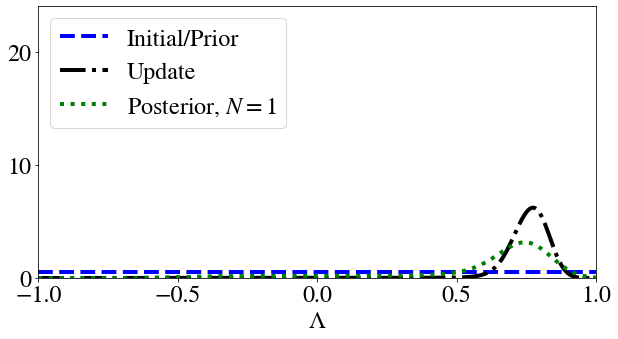
\includegraphics[width=0.49\linewidth]{figures/bip-vs-sip-1.png}
   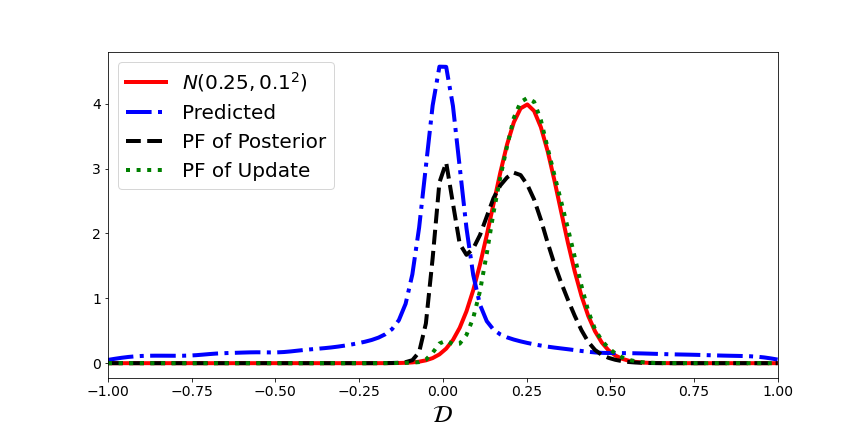
\includegraphics[width=0.49\linewidth]{figures/bip-vs-sip-pf-1.png}
 \caption{(Left) The initial/prior PDF $\initial$ (blue solid curve), updated PDF $\updated$ (black dashed curve), and posterior PDF $\pi_\text{post}$ (green dashed-dotted curve) on $\Lambda$.
 (Right) The push-forward (PF) of the initial/prior PDF $\predicted$ (blue solid curve), observed/likelihood PDF (red solid curve), PF of the updated PDF $\updated$ (black dashed curve), and the PF of the posterior PDF $\pi_\text{post}$ (green dashed-dotted curve) for the QoI.}
 \label{fig:bayes-comparison}
\end{figure}


While the updated and posterior densities in Fig.~\ref{fig:bayes-comparison} share certain similarities (e.g., they are uni-modal with similar locations of the mode), they are otherwise visibly distinct.
The differences between these densities is made more evident by examining their push-forwards.
The push-forward of the updated density agrees well with the observed density, which is to be expected.
However, the push-forward of the posterior is bi-modal and does not match the observed density, which we recall is identical to the data-likelihood function in this case.
%with peaks that appear to align fairly well with the two distinct peaks of the predicted density and observed density.
%Recall that the observed density and data-likelihood are, in this case, identical.
%Moreover, with the setup described above, the predicted density can also be interpreted as the push-forward of the prior density.
%This demonstrates the regularizing impact of the prior on the posterior and how i.

%
%Hierarchical Bayesian methods \cite{} extend this typical framework to problems where aleatoric uncertainties are present, but are still fundamentally developed from a  point estimation perspective.
%Specifically, prior distributions are specified from a parametric family of distributions, such as Gaussian distributions, and the hyper-parameters used to define that family of distributions, such as the means and variances, become a focal point of estimation by the methodology.

\end{ex}

The takeaway to the above discussion and example is that each density is solving a {\em different} inverse problem.
The posterior density is intended to provide point estimates of a true parameter value whereas the updated density is intended to quantitatively characterize natural variations in parameter values.
We reformulate the previous example to make the role of data collection more central in the follow example.

\begin{ex}
For the (Bayesian) Deterministic Inverse Problem, suppose $Q(\paramref)=0.25$ and noisy measurement data are drawn from a $N(0.25,0.1^2)$, i.e., we assume that each datum is given by $d=Q(\paramref)+\xi$ where $\xi\sim N(0,0.1^2)$.
For the SIP, we use the sample mean and variance of data to estimate the ``exact'' observed $N(0.25,0.1^2)$ distribution.
The observed density and data-likelihood are significantly different from one another, especially as more data are collected.
The data-likelihood is given by a product of normal densities.

We draw $M=5, 10, \text{ and}, 20$ samples to form estimates of $\observed$ and the likelihood functions.
We show the results in Figure~\ref{fig:bayes-comparison-convergence}.

\begin{figure}[htbp]
\centering
   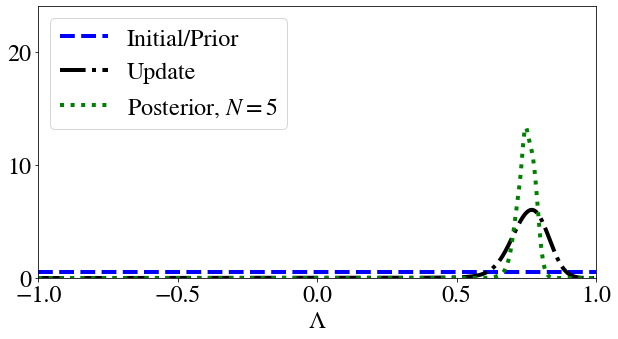
\includegraphics[width=0.49\linewidth]{figures/bip-vs-sip-5.png}
   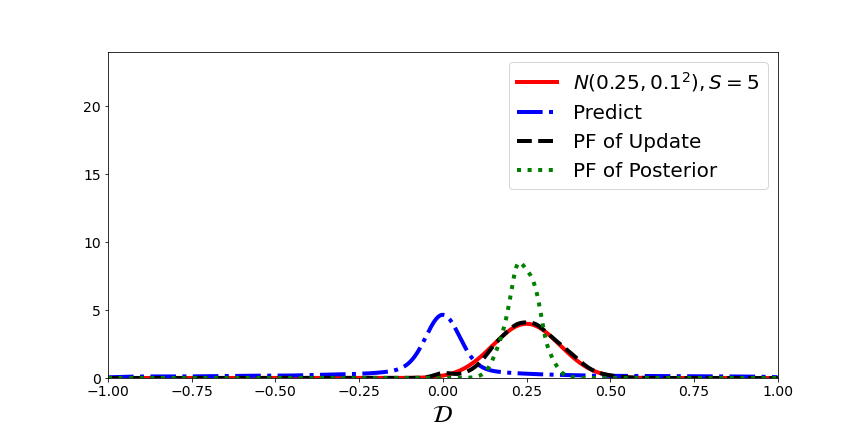
\includegraphics[width=0.49\linewidth]{figures/bip-vs-sip-pf-5.png}
   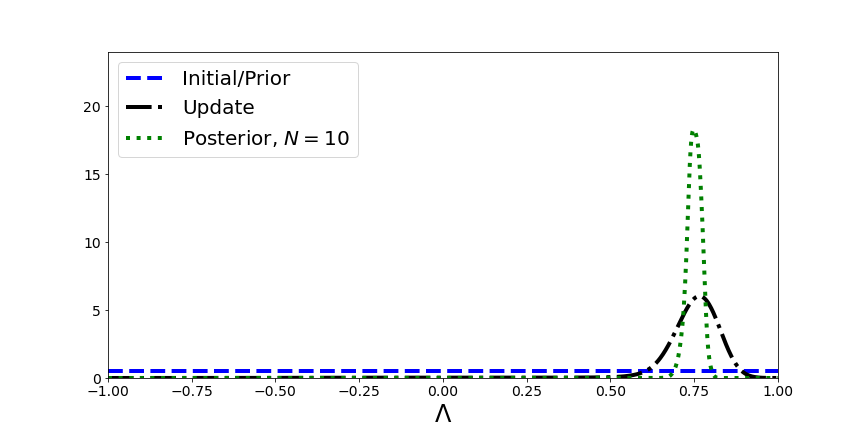
\includegraphics[width=0.49\linewidth]{figures/bip-vs-sip-10.png}
   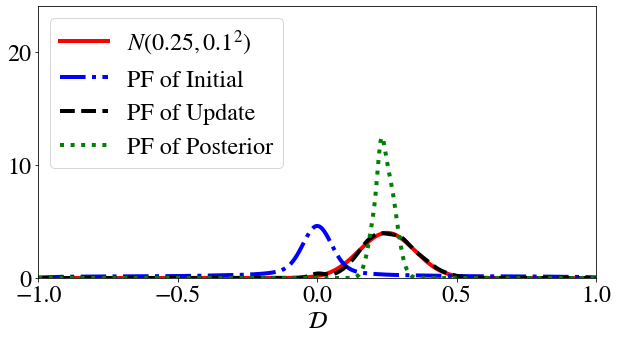
\includegraphics[width=0.49\linewidth]{figures/bip-vs-sip-pf-10.png}
   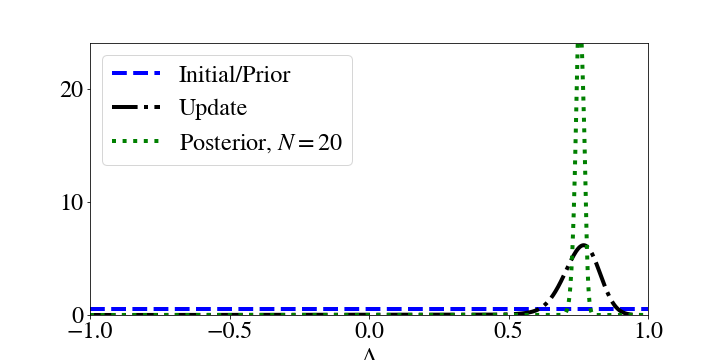
\includegraphics[width=0.49\linewidth]{figures/bip-vs-sip-20.png}
   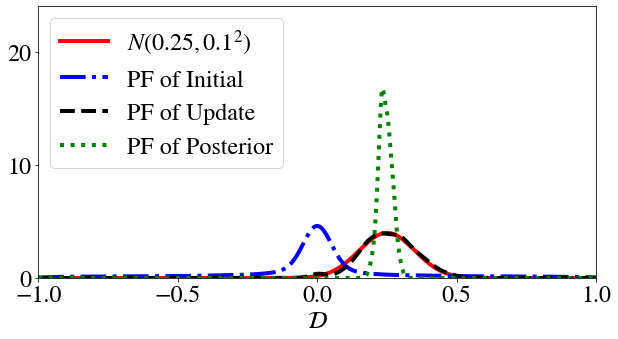
\includegraphics[width=0.49\linewidth]{figures/bip-vs-sip-pf-20.png}
 \caption{(Top to Bottom): $S=5, 10, \text{ and}, 20$ samples are used to solve the SIP and DIP for comparison. (Left) The initial/prior PDF $\initial$ (blue solid curve), updated PDF $\updated$ (black dashed curve), and posterior PDF $\pi_\text{post}$ (green dashed-dotted curve) on $\Lambda$.
 (Right) The push-forward (PF) of the initial/prior PDF $\predicted$ (blue solid curve), observed/likelihood PDF (red solid curve), PF of the updated PDF $\updated$ (black dashed curve), and the PF of the posterior PDF $\pi_\text{post}$ (green dashed-dotted curve) for the QoI.}
 \label{fig:bayes-comparison-convergence}
\end{figure}

For all values of $M$, the push-forward of the initial remains the same, and the push-forward of the update matches the observed.
By contrast, the posterior increases in confidence alongside the predictions it produces.
This further illustrates the point made earlier: the DIP and SIP are solving fundamentally different problems (they are addressing different questions).
The mean of the updated density could be used as an estimator to address the parameter identification problem, but collecting more data does not improve confidence.
As more data is incorporated, the goal of the DIP is to reduce epistemic uncertainty; for the SIP, it is to quantify the aleotoric uncertainty.

\end{ex}




%%%%%

In summary, it is not the goal of Bayesian inference to construct a pullback distribution.
Bayesian inverse problems are fundamentally posed as parameter-identification, not distribution estimation.
However, one could assume that a posterior on $\pspace$ can be expressed as a Gaussian distribution, and solve for the most likely mean and standard deviation that characterizes it [TK - cite more] \cite{Smith}.
This defines what is commonly referred to a as a Hierarchical Bayesian Inverse Problem.
More complex densities can be approximated by mixture models.

For example, one can assume that the posterior can be given by a linear combination of four Gaussian distributions, and solve for eight parameter values (four standard deviations and means).
However, the operative word here is \emph{assume}; in order to capture a density using a Bayesian framework, one needs to impose some sort of explicit structure on the posterior.
No such compromise is required in the DCI framework.
Distributions (or measures) can be solved for directly, regardless of any nonlinear/non-parameteric structure by leveraging the measure-theoretic approach described in \cite{BE13} or \cite{BJW18}.

It is important to note that Hierarchical Bayesian inverse problem casts a distribution-estimation problem in the context of parameter identification.
As a complementary line of reasoning, we seek to formulate a parameter identification problem in a DCI framework.
We revisit the results with a focus on parameter estimation using $\updated$. [TK - not sure what Troy's comment here means]

In Chapter~\ref{chapter:mud}, we motivate the use of the maximal updated density point (maximizing the update), as a means of providing a useful point estimate to parameters.
Before we proceed, we finish presenting some summarizing key results about the stability and numerical convergence of the updated solution \eqref{eq:updated-pdf} in the next section.

\FloatBarrier

\section{Properties and Assumptions of Consistent Update}\label{sec:properties}
Recall that the SIP is defined as finding a measure $\PP_\pspace$ such that the push-forward of it matched $\observedP$.
The following assumption guarantees the existence of a solution to the SIP in the form of an update to the initial distribution.
It implies that any event which is assigned a positive probability by the observations must also have a positive predicted probability.

\begin{assumption}[Predictability Assumption (Theoretical Form)]\label{as:predicted-theoretical}
  The measure associated with $\observed$ is absolutely continuous with respect to the measure associated with $\observed$.
\end{assumption}

If this is unsatisfied, one source of information (the data) suggests certain events are probable while another source of information (the model and initial beliefs) have a priori ruled that almost surely these events should not occur.
Therefore, either initial beliefs, the model under consideration, or the description of uncertainty encoded in $\predicted$ should be subjected to a critical reevaluation.

The following establishes a more practical form (from the perspective of numerical implementation), of \ref{as:predicted-theoretical} which states that the predicted measure must dominate the observed.
\begin{assumption}[Predictability Assumption (Practical Form)]\label{as:predicted-practical}
The requirement given in Assumption~\ref{as:predicted-theoretical} is guaranteed if the following is satisfied:
\begin{equation}\label{eq:pred-pract}
  \exists \; C>0 \text{ such that } \observed (\q) \leq C \predicted(\q) \text{ for a.e. } d\in \dspace,
\end{equation}
where it is understood that $\q = \qlam$ for some $\param \in \pspace$.
\end{assumption}

Assumption~\ref{as:predicted-practical} is particularly useful in that it is the same condition required for applying rejection sampling, which we summarize in Algorithm~\ref{alg:rejection}.
Specifically, this allows us to sample from the updated density using the initial density as follows:

\begin{algorithm}[hbtp]
\DontPrintSemicolon
Draw $\nsamps$ independent identically distributed (i.i.d.) initial samples from the initial density
	\For{$\iparam = 1, \hdots, \nsamps$}{
	    Compute $\Qi = \qoi(\param^{(\iparam)})$.\\
	}
	Approximate $\predicted$, the push-forward of $\initial$, by some method such as kernel density estimation.
  \For{$\iparam = 1, \hdots, \nsamps$}{
	    Compute $r\lami = \frac{\observed\Qi}{\predicted\Qi}$.\\
	}
  Normalize $r$ by dividing it by $\max(r)$.
  \For{$\iparam = 1, \hdots, \nsamps$}{
      Draw a sample from a standard uniform distribution.
	    If the value of $r\lami$ exceeds the value of the random sample, keep $r\lami$.\\
	}
 \caption{Rejection Sampling Leveraging Ratio from Density-Based Approach}
 \label{alg:rejection}
\end{algorithm}

Now, assuming \eqref{eq:pred-pract} holds, we state the following theorem from \cite{BJW18a} based upon the disintegration of measures:

\begin{thm}[Existence and Uniqueness]
  For any set $A\in \pborel$, the probability measure $\updatedP$ defined by
  \begin{equation}\label{eq:dci_sol}
    \updatedP (A) = \int_\dspace \left (  \int_{\pspace \in \qoi^{-1}(\q)}  \initial\lam \frac{\observed\Q}{\predicted\Q} \, d\mu_{\pspace, \q} \lam \right ) \, d\dmeas(\q), \; \forall \; A \in \pborel
  \end{equation}
  is a consistent solution to the SIP given in (\ref{eq:inverse-problem}), and is uniquely defined up to the specification of the initial probability measure $\initial$ on $(\pspace, \pborel)$.
  Here, $\mu_{\pspace, d}$ denotes the disintegration of the dominating measure $\mu_\pspace$.
\end{thm}

The updated density \eqref{eq:update} in the iterated integral in \eqref{eq:dci_sol} has no normalization constant because it is in fact a density (i.e., it integrates to $1$), which is summarized in Corollary 3.1 in \cite{BJW18a} and restated in simplified form below:
\begin{cor}\label{cor:int}
$\updatedP(\pspace) = 1$.
\end{cor}

These definitions are combined to identify the form of the \emph{updated density}, originally derived in \cite{BJW18a}:

\begin{defn}[Updated Distribution]\label{defn:updated}
  A solution satisfying \eqref{eq:dci_sol} is referred to as an updated distribution, with an updated density
  \begin{equation}\label{eq:update}
    \updated \lam = \initial \lam \frac{\observed \Q }{\predicted \Q }, \; \forall \; \param \in \pspace.
  \end{equation}
\end{defn}

% Corollary~\ref{cor:int} is critical to understanding some significant differences between the classical Bayesian posterior density~\cite{Smith} and the updated density density given by \eqref{eq:update}, which we discuss in Section~\ref{sec:othermethods} as well as other places throughout this thesis.
% Moreover, this Corollary provides the basis for a useful numerical diagnostic that assesses both the quality of a numerical approximation of $\updated$ based on finite sampling and density estimation as well as any potential violations of the predictability assumption.

% We next turn our attention to attributes of the Data-Consistent framework which make it appealing for use in solving inverse problems.
% Namely, we summarize the stability results first presented in \cite{BJW18} that demonstrate that approximation errors in the updated density are well understood within the measure-theoretic foundation on which the approach is constructed.

%%%%%%%%%%%%%%%%%%%%%%%%

\subsection{Stability of the Consistent Solution}\label{sec:stability}
The Total Variation (TV) metric on a space of probability measures, absolutely continuous with respect to a dominating measure $\mu$, is defined as
\begin{equation}\label{eq:tv}
d_{\text{TV}} (\PP_f, \PP_g) := \int \abs{\pp_f - \pp_g} \, d\mu,
\end{equation}
where $\pp_f,\pp_g$ are the densities (Radon-Nikodym derivatives with respect to $\mu$), associated with measures $\PP_f, \PP_g$, respectively.
The stability results below are all with respect to the TV metric, which is widely used in the literature and is also known as \emph{statistical distance}~\citep{GS02, Smith, Silverman}.
We first define stability with respect to perturbations in the data.

\begin{defn}[Stability of Updated Densities I]\label{defn:stableobs}
  Given $\initialP$ and $\observedP$, let $\widehat{\observedP}$ be any perturbation to $\observedP$ on $(\dspace, \dborel)$ satisfying \eqref{eq:pred-pract}.
  Let $\updatedP$ and $\widehat{\updatedP}$ denote the consistent solutions associated with $\observedP$ and $\widehat{\observedP}$, respectively.
  We say that $\updatedP$ is \emph{stable} with respect to perturbations in $\observedP$ if for all $\eps > 0$, there exists a $\delta > 0$ such that
  \begin{equation}
    d_{\text{TV}} (\observedP, \widehat{\observedP}) < \delta \implies d_{\text{TV}} (\updatedP, \widehat{\updatedP}) < \eps.
  \end{equation}
\end{defn}

In \cite{BJW18a}, it is shown that $d_{\text{TV}} (\widehat{\updatedP}, \updatedP) = d_{\text{TV}} (\widehat{\observedP}, \observedP)$, which immediately proves the following:

\begin{thm}
  $\updatedP$ is stable with respect to perturbations to $\observedP$.
  \label{thm:stableobs}
\end{thm}

This next definition and result are useful in analyzing the sensitivity of the updated density with respect to the initial beliefs.

\begin{defn}[Stability of Updated Densities II]\label{defn:stableinitial}
  Given $\initialP$ and $\observedP$, let $\widehat{\initialP}$ be any perturbation to $\initialP$ on $(\pspace, \pborel)$ satisfying \eqref{eq:pred-pract}.
  Let $\updatedP$ and $\widehat{\updatedP}$ denote the consistent solutions associated with $\observedP$ and $\widehat{\observedP}$, respectively.
  Let $\sett{\PP_{\pspace, d}}{d\in\dspace}{}$ and $\sett{\widehat{\PP_{\pspace, d}}}{d\in\dspace}{}$ be the conditional probabilities defined by the disintegration of $\initialP$ and $\widehat{\initialP}$, respectively.
  We say that $\updatedP$ is \emph{stable} with respect to perturbations in $\initialP$ if for all $\eps > 0$, there exists a $\delta > 0$ such that for almost every $d\in\supp(\observedP)$,
  \begin{equation}\label{eq:stableinitial}
    d_{\text{TV}} (\PP_{\pspace, d}, \widehat{\PP_{\pspace, d}}) < \delta \implies d_{\text{TV}} (\updatedP, \widehat{\updatedP}) < \eps.
  \end{equation}
\end{defn}

The following important stability theorem is also proven in \cite{BJW18a}:

\begin{thm}
  $\updatedP$ is stable with respect to perturbations to $\initialP$
  \label{thm:stableinitial}
\end{thm}

Taken together, these stability results provide assurance that the updated density we obtain is accurate up to the level of experimental error polluting $\observedP$ and error in incorrectly specifying initial assumptions using $\initialP$.
Given that specifying the definition of a ``true'' initial density is somewhat nebulous, we are less interested in the consequences of the latter conclusion.
However, generating samples from $\updatedP$ generally requires a numerical approximation to the predicted distribution, which introduces additional errors in $\updatedP$.
In Section~\ref{sec:approx}, the TV metric is used to bound the error in the updated density in terms of the error in the approximation to the push-forward of the initial.




%%%%%%%%% Section 2.3
\subsection{Numerical Approximation and Sampling}\label{sec:approx}
%Since we are given $\initial$ and $\observed$, the computation of $\predicted$ is the only aspect of the Consistent Bayesian framework that needs to be approximated.
%Since there are few restrictions on the structure of the map $\qoi$ that defines $\predicted$, there is in general no explicit expression from which we can generate samples, so we use a numerical approximation to the probability density function.
%
%For simplicity, we simply propagate Monte-Carlo samples from the prior and use a kernel density estimate (usually Gaussian\footnote{In this proposal, all results are generated using this kernel, though six kernels common to density estimation are implemented in the ConsistentBayes Python package [TK - cite Silverman and your github].}).
%
%We summarize this in the following algorithm:
%
%\begin{algorithm}[hbtp]
%\DontPrintSemicolon
%Generate a set of samples $\sett{\param_i}{i=1}{N}$
%	\For{$i = 1, \hdots, N$}{
%			Propagate sample $\param_i$ through the QoI map. Set $d_i = \qoi(\param_i)$.
%	}
%Use $\sett{d_i}{i=1}{N}$ and a density estimation method to approximate $\predicted$.
%	\label{alg:sample}
%\caption{Numerical Approximation of the Push-forward of the Prior Density}
%\end{algorithm}
%


%The computational object associated with $\predicted$ is stored for re-use and can be evaluated at locations in $\dspace$ other than $\sett{d_i}{i=1}{N}$.
%This procedure should be thought of as a characterization of the data space given the prior assumptions encoded in $\initial$.

If $\widehat{\predicted}$ denotes a computational approximation to the push-forward of the initial density obtained with $\widehat{\predicted}$ substituted for $\predicted$ in \eqref{eq:dci_sol}, then the conditional densities from the Disintegration Theorem (c.f. Chapter~\ref{chapter:geometry} for more details), are given as
\[
\frac{\widehat{d\PP_{\pspace, d}}}{d\mu_{\pspace, d}\lam} = \frac{\initial\lam}{ \widehat{\predicted\Q} },
\]
where $\widehat{\PP_{\pspace, d}}$ denotes the disintegration of $\widehat{\updatedP}$.


We assume the following for the approximation of the push-forward of the initial density:
\begin{assumption}\label{as:predicted-theoreticalx}
There exists some $C>0$ such that
\[
\observed (d) \leq C \widehat{\predicted(d)} \text{ for a.e. } d\in \dspace.
\]
\end{assumption}

If this assumption is satisfied, then from \cite{BJW18a}, we have the following:
\begin{thm}\label{thm:predicted_bound}
  The error in the approximate updated density is bounded above:
  \begin{equation}\label{eq:predicted_bound}
    d_{\text{TV}} (\updatedP, \widehat{\updatedP}) \leq C d_{\text{TV}} (\predictedP, \widehat{\predictedP}),
  \end{equation}
  where the $C$ is the constant taken from Assumption \ref{as:predicted-theoreticalx}.
\end{thm}

A straightforward approach to construct $\widehat{\predicted}$ is to use a forward propagation of samples from $\pspace$ to $\dspace$ and then apply kernel density estimation (KDE)~\citep{BJW18a}.
Then, we may evaluate $\updated$ directly for any sample of $\pspace$ at the cost of one model solve per sample.
While this allows us to incorporate sophisticated sampling techniques such as Markov-Chain Monte-Carlo (MCMC)~\citep{Smith, Tarantola_book} to generate samples according to the updated distribution, we often opt for a simpler route based on rejection sampling by re-using the initial set of propagated samples.
This avoids any additional model evaluations (as would be required by techniques relying on proposal samples such as MCMC).
We leverage the re-use of samples in the results herein extensively.

By Theorem~\ref{thm:predicted_bound}, the accuracy of the computed updated density relies on the accuracy of the approximation of the push-forward of the initial.
Throughout this thesis, we utilize a KDE with a Gaussian kernel to produce the non-parametric estimates of $\predicted$.
Such KDEs are known to converge at a rate of $\mathcal{O}(N^{-4/(4+\dimD)})$ in mean-squared error and $\mathcal{O}(N^{-2/(4+\dimD)})$ in $L^1$-error, where $\dimD$ is the dimension of $\dspace$, and $N$ is the number of samples from $\initial$ propagated through $\qoi$ \citep{Silverman}.

For simplicity, we introduce the following notation to capture the role of the ratio involved in \eqref{eq:dci_sol} to demonstrate properties we can leverage for generating samples from $\updated$.
We let
\[
\updated\lam = \initial \lam r\Q, \text{ where } r\Q = \frac{\observed\Q}{\predicted\Q}.
\]

Many standard calculations about the updated density involve integrals of functions of $r\Q$ with respect to the prior.
For any measurable function $f$, we establish the connection of calculating quantities over $\pspace$ with those over $\dspace$ by leveraging the following identity:
\[
\int_\pspace f\left( r\Q \right ) \, d\initialP = \int_\dspace f\left( r(\q) \right ) \, d\predictedP
\]

We use several throughout this thesis, including the integral of the updated density:
\[
I(\updated ) = \int_\pspace r\Q \, d\initialP = \int_\dspace r(\q) \, d\predictedP ,
\]
which we can use to validate that $I(\updated) = 1$ in order to numerically validate that the predictability assumption given in \eqref{eq:predicted_bound} was not violated.
The sample average of $r(\q)$ can be used to estimate $I(\updated)$.
This convenience is afforded by the fact that the i.i.d. samples provide us with the ability to take a Monte-Carlo estimate of the integral.

% Similarly, we follow \cite{BJW18} to write the commonly used metric for Information Gain, the Kullback-Liebler (KL) divergence:
% \begin{equation}\label{eq:KLdiv}
% \text{KL}(\initial : \updated ) = \int_\pspace r\Q \log r\Q \, d\initialP = \text{KL}(\observed : \predicted ),
% \end{equation}
% i.e., the KL-divergence between the initial and updated density is equal to the KL-divergence between the observed and the predicted densities.

Taken together, the results summarized in this section demonstrate that the Data-Consistent framework and density-based solution \eqref{eq:dci_sol} have been rigorously constructed and studied.
They give an experimenter assurance that there are not unexpected consequences for small mistakes in problem formulation.
In the following section, we provide a similar sense of assurance for a central practical consideration involved in this work: that the results depend on computational implementations of the aforementioned theory, i.e., software.
We directly address how to establish a complementary level of rigor to the implementation of the work as was invested in the construction of the theory.
We leverage modern advances in software engineering with an emphasis on results being reproducible in an accessible manner.

\section{Towards a Reproducible Thesis}\label{sec:reproducibility}

\subsection{Motivations}\label{sec:motivations}
In some respects, the practice of writing software has diverged from the motivations of an academic researcher.
The latter seeks to generate new knowledge and may write a set of example scripts/programs to demonstrate some novel idea or method.
By contrast, the motivations of a software engineer are related to resiliency.
Not only must they ensure the code works as expected given a myriad of ways users may interact with it, but it is necessary to write the code in a manner compatible with maintaining it into the future.
Much of the work of writing ``good software'' is concerned with writing appropriate documentation to express the intended usage and logic underlying architectural decisions.
There are many ways to write a functioning program to demonstrate a proof-of-concept, but creating something that is \emph{user-friendly}, guaranteed to be free of mistakes, and scales across different computational environments/resources requires an entirely different approach.

Decisions made early in the software design cycle have lasting impacts on future features and functionality.
Rigor is added to libraries through the writing of \emph{unit tests}, and use of \emph{continous integration} ensures that the download and installation process is predictable and reproducible.
Code that only runs on the author's computer is impractical, since any thorough critique requires independent verification.
Without proper context and architecture, new ideas that are implemented in programs are unlikely to be adopted.


This thesis is concerned not only with a demonstration of novel mathematical content\---showcasing new ways to make inferences from noisy data in a novel Data-Consistent framework\---it also serves to document the process of ensuring that the work is \textbf{fully reproducible}.
In mathematics, reproducibility is ensured through the use of proofs, which motivate the original work presented here.
However, as the title of this thesis suggests, much of the focus is actually on the computational implementation of the novel research into Data Consistent Inversion, studying the impact of using computers to perform the task of making conclusions based on data.
Mathematics is implemented on computers through software.
We are therefore concerned with ensuring the expected functionality of that software, which aligns with our training as mathematicians; we care deeply about making sure things are rigorous.

In short, we want to make sure that theory aligns with practice, and that both live up to high standards of intellectual scrutiny.
Every computational result, illustrative figure, table, plot, etc. presented in this thesis is associated with the scripts that generate them, and are included in the  repository for this document [TK - cite].
It is written in \LaTeX~(which is itself a programming language), and presents its own software dependencies in addition to those required to run the scripts to generate the images and tables.
To address this concern, we leverage \emph{Travis}, a continuous integration service [TK-cite], to ensure that all figures can be generated and the \LaTeX\, document compiles into a PDF.

The same care is taken to ensure the reproducibility of all numerical results based on software.
An \emph{image} that contains a fully pre-built Linux software environment within which one can compile the thesis and run the code is available through the Docker Cloud registry [TK -cite].
The latter enables the ability to generate this thesis document in its entirety on any software platform that supports Docker (Windows, MacOS, Linux).
A cloud service called Binder [ TK - cite mybinder.org] allows one-click deployments in any web-browser, removing the need for any installation whatsoever for anyone wanting to reproduce the contents of this document.




%%%%%%%%%%%%%%%%%%%%%%%%%%%%%%%%%%%%%%%%%%%%%%%%%%
\section{Outline of Remaining Chapters}\label{sec:outline}
In Chapter~\ref{chapter:mud}, we propose a way by which parameter identification can be performed in the DCI framework by posing the problem as a SIP and maximizing $\updated$.
Central to how this contribution is accomplished in practice is the definition of a data-constructed QoI map.
The impact of a QoI's inherent geometric properties on our ability to approximate solutions to SIPs using finite sampling is then summarized in Chapter~\ref{chapter:geometry}.
The focus there is on the property called skewness, which is connected to the QoI maps introduced in \ref{chapter:mud} through a case study of a PDE-based example in Chapter~\ref{chapter:vector-valued}.
Finally, we provide some concluding remarks and directions for future research in Chapter~\ref{chapter:future} alongside several examples demonstrating preliminary results for novel extensions of the work presented in this thesis.


\FloatBarrier

% \chapter{\uppercase{Background on Observation-Consistent Inversion} \label{chapter:02}}
% 
% \section{Notation, Terminology, and Assumptions}
% \subsection{Models and Parameters}
% We begin by assuming that a (deterministic) model, denoted by $$\M (u, \param) = 0,$$ is specified to relate observable state variables $u$ to model inputs ({\em parameters}) denoted by the vector $\param\in\RP$.
% The components $\param_\iparam$ may include parameters in either the model operator (e.g. a diffusion coefficient) or input data (e.g. the frequency of a sinusoidal source, initial, or boundary information).
% We let $\pspace$ denote the set of all possible input parameters.
% We assume $\pspace\subset\RP$ is equipped with a (dominating) measure, $\pmeas$ on the Borel $\sa$ $\pborel$, defining the measure space $\Pspace$.
% The solution operator of the model $\M$ then defines a map taking $\param\in\pspace$ to a solution, denoted $u\lam$, to make explicit the dependence on $\param$, which is assumed to be unique.
% 
% However, in real experimental settings we are often unable to fully observe $u\lam$.
% Instead, we often only have access to some finite set of observable scalar quantities.
% For example, in experiments involving the diffusion of heat, we can typically only record the temperature at some small number of pre-specified points in space-time where measurement devices can be positioned.
% 
% \subsection{Quantities of Interest}
% Such observable values of $u\lam$ are mathematically modeled by functionals of the solution, denoted $\qoi_\idata: u\lam \to \RR$.
% The collection of such functionals into a vector defines a {\em Quantity of Interest} (QoI) map.
% Since the solution to the model depends on $\param$, so do the QoI, which motivates the notation
% $$\qlam := \qoi( u\lam ) \in\RD,$$
% to make this dependence on model parameters explicit.
% Furthermore, this convention captures a realistic limitation of an experimental setting, where we may be able to control $\param$ in order to observe $\qlam$, but lack the ability to observe $u\lam$ directly.
% The outputs of the QoI map $\qlam = \data$ are what we refer to as the \emph{data}.
% Similarly, the range of the QoI defines the \emph{data space} $\dspace$, i.e.
% $$\dspace = \qoi(\pspace) \subset \RD$$
% 
% We let $\qspace$ denote the set of possible QoI maps for which it is possible to collect experimental data.
% For example, suppose we can record only a single temperature measurement at any of ten locations in space-time.
% Then $\qspace$ is defined by ten possible QoI maps.
% If we can record any two such measurements, then $\qspace$ is defined by $\binom{10}{2} = 45$ possible maps.
% Observe that $\qspace$ could easily be uncountable\--for example if we were not limited to the spatial locations (or time) at which we could record temperature measurements.
% However, for simplicity, we will only discuss problems where $\qspace$ is finite.
% In the event that we need to compare maps, we adopt the notation $\dspace_{\qoi}$ to emphasize that the data space depends on the choice of QoI map $\qoi$; when the context is clear, we drop the subscript.
% The only assumption on $\qoi$ that we impose throughout this work is that of piecewise-differentiability.
% 
% \subsection{Chapter Outline}
% First, to reflect the order in which these results were researched and developed, we discuss set-based inversion.
% In the interest of clarity of exposition, we have adapted the notation of a sample-based approach developed later to express the construction of the former.
% Consequently, the references cited may require some work translating to match the notation we used.
% Similarities and differences between the two approaches has heretofore avoided formal documentation due to the novelty of the observation-consistent approach, particularly with respect to its use for epistemic uncertainty quantification, and this work serves to lay the groundwork for such a comparison.
% 
% In this chapter, we discuss the issues that arise from the need to numerically approximate the solutions to our inverse problems, and study the implications in \ref{sec:set-error} and \ref{sec:sample-error}.
% Discussion of the impact of sample size are kept to a minimum in this chapter in the interest of restricting the scope of chapter \ref{chapter:03} to the implications for convergence of (consistent) solutions to \eqref{eq:inverse-problem}.
% 
%%%%%%%%%%%%%%%%%%%%%%%%%%%%%%%%%%%%%%%%%%%%%%%%%%%%%%%%%%%%%%%%%%%%%%

%%% THIS GOES TO CH4 NOW %%% 
%\section{Set-Based Inversion for Measures}\label{sec:ch02-set}
% Intro
%To properly summarize the Stochastic Inverse Problem (SIP) and desired solution, we define several measure/probability spaces and refer to the schematic given in Figure \ref{fig:scheme}\---borrowed from \cite{BM17}\---in order to illustrate the steps and spaces required in the formulation and solution of the SIPs we consider herein.
For a more extensive review, we refer the reader to \cite{BBE11}, \cite{BES12}, \cite{BET+14}, and \cite{BM17}.

%%%%%%%%%%%%%%%%%%%%%%%%
\begin{figure}[!h]
\begin{equation}
\underbrace{
\underbrace{
\overbrace{
 \Pspace \xmapsto{\  Q \ } \Dspace
  \xmapsto{\ \dataP \ } (\dspace, \dborel, \dataP)
 }^{
 \text{(S1): Stochastic Inverse Problem (SIP)}
 }
 \xmapsto{\ Q^{-1} \ } (\pspace, \cborel, \contourP)
 }_{
 \text{(S2): Solution to SIP Satisfying Eq. \eqref{eq:dataspace_pushforward_measure}}}
 \xmapsto{\ \set{\PP_\ell}_{\ell\in\mathcal{L}} \ } (\pspace, \pborel, \paramP)
 }
 _{
 \text{(S3): Unique Solution to SIP by Eq.~\eqref{eq:disintegration_measure} and Ansatz}
 }
\end{equation}
\caption{The first step (S1) defines (i)~the formulation of the SIP by specification of the model, (ii)~the measure spaces of parameters and (iii)~observable outputs, and (iv)~the probability measure on the latter. The second step (S2) defines a unique solution to the SIP on the space $\pspace$ equipped with the contour $\sa$ $\cborel$ using the definition of the push-forward measure. In (S3), the Disintegration Theorem and and Ansatz are applied to define a unique solution on the space of interest $(\pspace, \pborel)$ equipped with a probability measure $\paramP$.}
\label{fig:scheme}
\end{figure}


The initial measure/probability spaces involved in the formulation of the SIP are summarized in step (S1) of Fig.~\ref{fig:scheme}, starting with measure space $\Pspace$.

The assumption that $\qoi$ is at least piecewise-differentiable implies the measurability of the QoI map, so that the space $\dspace$ induced by $\qoi$ is equipped with the Borel $\sa$ $\dborel$ [TK - cite textbook].
The ``push-forward'' measure $\dmeas$ on ${(\dspace, \dborel)}$ is defined as
\begin{equation}\label{eq:dataspace_pushforward_measure}
\dmeas (A) = \int_A \, d\dmeas := \int_{\qoi^{-1}(A)} \, d\pmeas = \pmeas \left (\qoi^{-1}(A) \right ) \quad \forall \;  A\in\dborel,
\end{equation}
which defines the measure space $\Dspace$\footnote{When referring to properties of the data space that are not unique to the choice of map used to induce $\dspace$, we will drop the subscript notation and assume the dependence is understood, as expressed in Fig.~\ref{fig:scheme}.}.
The push-forward distribution $\partial \dataP / \partial \mu_D$ is referred to as the \emph{predicted} distribution and is given by the Radon-Nikodym derivative with respect to (the Lebesgue) volume measure $\mu_D$ on ${(\dspace, \dborel)}$

The final step in (S1) involves the specification of a probability measure $\dataP$ on ${(\dspace, \dborel)}$ to model the uncertainty in data.
We colloquially refer to the distribution (given by the Radon-Nikodym derivative $\partial \dataP / \partial \pmeas$) as the \emph{observed} distribution, where $\pmeas$ is taken to be the (Lebesgue) volume measure on ${(\pspace, \pborel)}$.
This leads to the following SIP: determine a probability measure $\paramP$ on ${(\pspace, \pborel)}$ such that the push-forward measure of $\paramP$ matches $\dataP$.

In other words, determine a $\paramP$ satisfying
\begin{equation}\label{eq:inverse_measure}
\paramP \left ( \qoi^{-1}(E)\right ) = \PP_{\dspace}(E) \; \forall \, E \in \dborel.
\end{equation}

We call any such solution $\paramP$ to Eq.~\eqref{eq:inverse_measure} a (measure-theoretic) solution to the SIP.
This equation implies that any solution is uniquely determined on the induced contour $\sa$
\begin{equation}\label{eq:contour_sa}
\cborel = \set{\qoi^{-1}(E) : E \in \dborel } \subset \pborel,
\end{equation}
which is summarized as step (S2) of Fig.~\ref{fig:scheme}.

However, for sets $A \in \pborel \setminus \cborel$, more information is required than is provided in Eq.~\eqref{eq:inverse_measure} in order to determine $\paramP (A)$.
By the Implicit Function Theorem, if $\data \in C^1 (\pspace)$ and we let $\data\in\dspace$ be a fixed datum, $\qoi^{-1}(q)$ exists as a $(\nparams-\ndata)$\--dimensional manifold (possibly piecewise-defined) that we refer to as a \emph{generalized contour} \cite{BET+14}.
These generalized contours can be indexed by a manifold (also possibly piecewise-defined) of dimension $\ndata$ called a \emph{transverse parameterization} that intersects each contour once and only once.
In \cite{BET+14}, it is shown that transverse parameterizations are guaranteed to exist but are in general not unique.

We let $\LL$ denote any particular transverse parameterization.
Each $\ell\in\LL$ corresponds to a unique generalized contour $\CC_\ell \in \pspace$ and each point $\param\in\pspace$ belongs to a unique $\CC_\ell\in\pspace$.
Thus, a transverse parameterization defines a bijection between the manifold $\LL$ and the partitioning of $\pspace$ into generalized contours.
The induced $\sa$ $\cborel$ and this bijection can then be used to define the measurable space $(\LL, \BB_\LL)$.

We denote the projection map $P_\LL : \pspace \to \LL$, and let $\set{\CC_\ell}_{\ell\in\LL}$ represent the family of generalized contours indexed by $\LL$, yielding the associated family of measurable spaces $\set{\left ( \CC_\ell, \BB_{\CC_\ell} \right )}_{\ell\in\LL}{}$.
A Disintegration Theorem [TK - cite] is then leveraged to define a unique decomposition for any $\paramP$ defined on $(\pspace, \pborel)$ as a (marginal) probability measure $\PP_\LL$ on $(\LL, \BB_\LL)$ and a family of (conditional) probability measures $\set{\PP_\ell}_{\ell\in\LL}$ on $\set{\left ( \CC_\ell, \BB_{\CC_\ell} \right )}_{\ell\in\LL}$ such that
\begin{equation}\label{eq:disintegration_measure}
\paramP (A) = \int_{P_\LL(A)} \left ( \int_{P_{\LL}^{-1} (\ell) \cap A}\, d\PP_\ell(\param) \right )\, d\PP_\LL (\ell), \; \forall \; A \in \pborel
\end{equation}

The uniqueness of a probability measure $\paramP$ on ${(\pspace, \cborel)}$ satisfying Eq.~\eqref{eq:inverse_measure} implies the uniqueness of the marginal probability measures $\PP_\LL$ for any particular specification of $\dataP$ on ${(\dspace, \dborel)}$.
The disintegration of Eq.~\eqref{eq:disintegration_measure} implies that a specification of a family of conditional probability measures $\set{P_\ell}_{\ell\in\LL}$ gives us a unique solution to the SIP on ${(\CC_\ell, \BB_{\CC_\ell})}$.

However, the conditional measures cannot be determined by solely by the specification of $\data\in\dspace$.
We follow the work of \cite{BET+14} and adopt the \emph{standard ansatz} determined by the disintegration of the volume measure $\pmeas$ to compute probabilities of sets contained within contour events.
The standard ansatz is given by
\begin{equation}\label{eq:standard_ansatz}
\PP_\ell = \mu_{\CC_\ell} / \mu_{\CC_\ell}(\CC_\ell), \; \forall \; \ell \in \LL,
\end{equation}
where $\mu_{\CC_\ell}$ is the disintegrated volume measure on generalized contour $\CC_\ell$.
Thus, we have defined a unique solution to the SIP on ${(\pspace, \pborel)}$, completing step (S3) in Fig.~\ref{fig:scheme}.

%% \subsubsection{Alternative Derivation Using Bayes' Rule}\label{sec:set_bayes}
In the measure-theoretic approach studied in~\cite{BBE11, BET+14}, Voronoi-cell discretizations of $\pspace$ are used to construct set-valued approximations of the updated measure directly, so we refer to it as the \emph{explicit} approach.
By contrast, sampling from densities is an \emph{implicit} approach, and is discussed in greater detail in \ref{sec:ch02-sample}.
Here, we provide a ``set-based'' derivation of the updated measure to more easily compare to the explicit approximation of the solution given measure in~\cite{BET+14}.

First, we start by observing that if $A, B \subset \pspace$ such that $A = \qoi^{-1}(\qoi(B))$, then we have that $B\subset A$ (the inclusion may be proper).
Therefore, for any probability measure $P$ on $(\pspace, \pborel)$, 
\[
P(B) = P(B|A) \, P(A).
\]
If $P$ is intended to solve the inverse problem, then we are motivated to take
\[
P(A) = \observed (\qoi(A)) = \observed (B),
\]
in the above formula.

We must now determine how to properly define $P(B|A)$. 
We leverage Bayes' Theorem~\cite{Smith} in order to utilize the prior density on contour events.
In other words, we use the prior $\initialP$ on $(\pspace, \pborel)$ and Bayes' Theorem to get
\begin{equation}\label{eq:bayes_full}
P(B|A) = \initialP(B|A) = \frac{ \initialP(A|B) \initialP(B) }{ \initialP(A) },
\end{equation}
and since $B \subset A$, $\initialP(A|B) = 1$, \eqref{eq:bayes_full} simplifies to

\begin{equation}\label{eq:bayes}
\initialP(B|A) = \frac{ \initialP(B) }{ \initialP(A) }.
\end{equation}

Recall from \eqref{eq:predicted} that $\predictedP$ is the push-forward of the prior, giving $\initialP(A) = \predictedP (\qoi(A)) = \predictedP \left (\qoi(B)\right )$, which then gives the following set-valued ``solution'' to the stochastic inverse problem:
\begin{equation}\label{eq:sip_sol_cont}
\updatedP(B) := \begin{cases}
\initialP(B) \frac{ \observed(B) }{ \predictedP \left (\qoi(B)\right ) ) } & \text{ if } \initialP(B) > 0,\\
0 & \text{ otherwise}.
\end{cases}
\end{equation}

This set-valued update is only a solution on certain (sub-)$\sigma$-algebras of $\pborel$. 
Nonetheless, we can form explicit approximations to the update, e.g. as done in~\cite{BET+14, BES12, BBE11}. 
In other words, an Ansatz is used in place of the prior; it serves the same purpose to distribute probabilities in directions not informed by the QoI map.

However, such an explicit approach requires an approximation of \emph{events in $\pborel$}. 
This is in direct contrast to the numerical approximation of the density $\updated$ that only requires approximation of $\predicted$.
Since we often expect the dimension of $\dspace$ to be less than the dimension of $\pspace$, this can prove to be a significant numerical advantage for the ``implicit'' approximation given by the updated probability density function. 

% Numerical Approximation
%\subsection{Numerical Approximation and Analysis}\label{sec:set-algorithm}
We present a non-intrusive algorithm based on Monte-Carlo sampling\---initially introduced in \cite{BET+14} and further analyzed in \cite{BET+14-arxiv}\---that is structured in four stages (written as four independent for-loops) that are linked to the stages in Fig.~\ref{fig:scheme}.
We direct the interested reader to \cite{BET+14-arxiv} for more detailed information and analysis of this algorithm, e.g., on the requirement of a sampler being ``$\pborel$-consistent'' to ensure convergence.


\begin{algorithm}[hbtp]
\DontPrintSemicolon
Choose a discretization partition $\set{D_\idisc}_{\idisc=1}^{\ndiscs}$ of $\dspace$.\\
	\For{$\idisc = 1, \hdots, \ndiscs$}{
			Compute $p_{\dspace, \idisc} = \dataP(D_\idisc)$.
	}
	Choose samples $\set{\param^{(\iparam)}}_{\iparam=1}^{\nsamps} \subset \pspace$, which implicitly defines a Voronoi-cell partition $\set{\VV_\iparam}_{\iparam=1}^{\nsamps}$ of $\pspace$.\\
	\For{$\iparam = 1, \hdots, \nsamps$}{
	Compute $\qoi_\iparam = \qoi(\param^{(\iparam)})$.\\
	Let $\OO_\idisc = \set{\iparam: \qoi_\iparam \in D_\idisc}$.\\
	Compute approximations $V_\iparam \approx \pmeas (\VV_\iparam)$.
	}
	\For{$\idisc = 1, \hdots, \ndiscs$}{
	Compute $\CC_\idisc = \set{\iparam:Q_\iparam \in D_\idisc}$.
	}
	\For{$\iparam = 1, \hdots, \nsamps$}{
	Compute $p_{\pspace, \iparam} = \left ( V_\iparam / \sum_{j\in \CC_{\OO_\iparam} } V_j \right ) p_{\dspace, \OO_\iparam}$.
	}
	For any $A\in \pborel$, compute
	\begin{equation}
	\PP_{\pspace, \ndiscs, \nsamps} (A) = \sum_{\iparam=1}^\nsamps p_{\pspace, \iparam} \Chi_{\VV_\iparam} (A)
	\end{equation}
 \caption{Numerical Approximation of the Inverse Density}
 \label{alg:inv_density}
\end{algorithm}


The first two stages correspond to formulating the discretized version of the SIP given in step (S1) in Fig.~\ref{fig:scheme}.
We first discretize the probability space $\Ospace$.
Then, we simultaneously discretize the measure space $(\pspace, \pborel, \pmeas)$ and construct a simple-function approximation to the map $\qoi$.
These stages introduce the primary sources of error, and the third and fourth stages may be thought of as solving the discretized SIP exactly.
The samples that are used to describe $\pspace$ implicitly define a set of Voronoi cells $\set{\VV_\iparam}_{\iparam=1}^{\nsamps}$, which can be seen in Figure~\ref{fig:voronoi_cells}.
Each sample set defines a fundamentally different geometry.

\begin{figure}[ht]
\centering
	\begin{minipage}{.475\textwidth}
		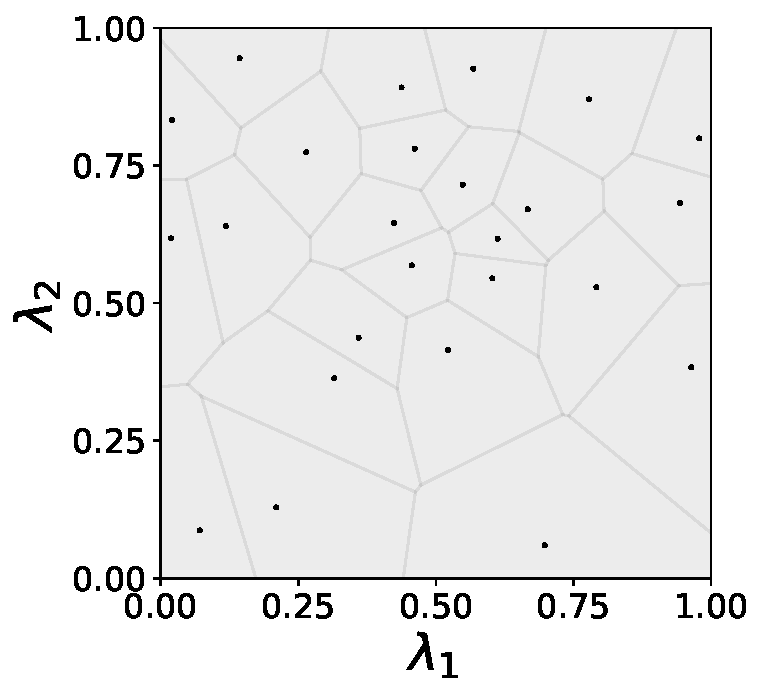
\includegraphics[width=\linewidth]{./images/voronoi_diagrams/voronoi_diagram_N25_r0}
	\end{minipage}
\caption{
Voronoi-cell discretization (partition) induced by $\nsamps = 25 $ uniform i.i.d.~random samples in $\pspace = [0,1]^2$.
}
\label{fig:voronoi_cells}
\end{figure}

The third stage then identifies the collection of Voronoi cells in $\pspace$ that approximate the contour events in $\cborel$ defined by $\qoi^{-1}(D_\idisc)$ for $\idisc=1,\hdots,\ndiscs$. This allows us to formulate the consistent solution to the discretized SIP on $(\pspace, \cborel, \contourP)$ as illustrated in step (S2) of Fig.~\ref{fig:scheme}.
Finally, the fourth stage\---associated with step (S3) in Fig.~\ref{fig:scheme}\---uses a discrete version of the ansatz to approximate the probability of $\VV_\iparam$ for $\iparam=1,\dots,\nsamps$.
This results in an approximate probability measure, denoted by $\PP_{\pspace, \ndiscs, \nsamps}$, which produces the same probability estimates for events $A$ and $A\setminus \set{ \param^{(\iparam)} }_{\iparam=1}^\nsamps$, which are identical almost everywhere with respect to $\pmeas$.

Note that Algorithm~\ref{alg:inv_density} makes no mention of the method by which the samples $\set{ \param^{(\iparam)} }_{\iparam=1}^{\nsamps}$ were generated or sets in $\set{D_\idisc}_{\idisc=1}^{\ndiscs}$ are chosen.
$\set{ \param^{(\iparam)} }_{\iparam=1}^{\nsamps}$ may be generated using uniform random sampling, latin hypercube sampling, or even regular grids.
A thorough discussion of the choices involved in making such decisions is beyond the scope of this work, though we touch briefly on the discretization of $\dspace$ below.


% Descriptions of Error
%\subsection{Descriptions of Error}\label{sec:set-error}

Recall that we assumed $\dataP$ is absolutely continuous with respect to $\dmeas$, which allows us to describe $\dataP$ with a density $\rho_\dspace$. Then, for any partition $\set{D_\idisc}_{\idisc=1}^{\ndiscs}$ of $\dspace$,
\[
\dataP (D_\idisc) = \int_{D_\idisc} \rho_\dspace \, \dmeas, \quad \text{ for } \idisc = 1, \hdots, \ndiscs.
\]

We often use Monte Carlo approximations to compute the approximations $p_{\dspace, \idisc}=\dataP(D_\idisc)$ in the first for-loop in Algorithm~\ref{alg:inv_density}.
These samples are generated on $\dspace$ and do not require numerical solutions to the model.
We therefore assume that for any discretization of $\dspace$, these approximations can be made sufficiently accurate and neglect the error in this computation.

We denote the exact solution to the SIP associated with this partitioning of $\dspace$ by $\PP_{\pspace, \ndiscs}$.
In situations where $\qoi(\param^{(\iparam)})$ is estimated (e.g. by application of a functional on a finite-element solution to a PDE), the approximate solutions to the SIP given in the final for-loop of Algorithm~\ref{alg:inv_density} are denoted by $\PP_{\pspace, \ndiscs, \nsamps, h}$.
Here, the $h$ is in reference to a mesh or other numerical parameter that determines the accuracy of the numerical solution $u_h(\param^{(\iparam)})\approx u(\param^{(\iparam)})$, and subsequently the accuracy in the computations of $\qoi_\iparam = \qoi(\param^{(\iparam)})$ in Algorithm~\ref{alg:inv_density}.

We assume that $h$ is tunable so that for any $A\in \pborel$,
\[
\lim\limits_{h \downarrow 0} \PP_{\pspace, \ndiscs, \nsamps, \imesh} (A) = \PP_{\pspace, \ndiscs, \nsamps} (A).
\]
It is possible to prove the convergence of $\PP_{\pspace, \ndiscs, \nsamps, \imesh} (A) \to \paramP (A)$ for some $A\in \pborel$ and on estimating the error in $\PP_{\pspace, \ndiscs, \nsamps, h}(A)$.
For example, in \cite{BGE+15}, adjoint-based a posteriori estimates in the computed QoI are combined with a statistical analysis to both estimate and bound the error in $\PP_{\pspace, \ndiscs, \nsamps, \imesh} (A)$.
In [TK - cite ISNME 2019], adjoints are used to compute both error and derivative estimates of $\qoi(\param^{(\iparam)})$ to improve the accuracy in $\PP_{\pspace, \ndiscs, \nsamps, \imesh} (A)$.
However, no work has to date fully explored the \emph{convergence rates} of Algorithm \ref{alg:inv_density}.
Furthermore, no work has yet to establish that these rates are independent of the choice of QoI map despite other studies establishing that the absolute error is very much affected by the geometric properties of the QoI maps [TK - cite Lindley + Butler].

In order to study convergence, we need to define a notion of distance on the space of probability measures on $\pspace$, which we denote by $\PPspace$.
% There are many choices available to us and we discuss several useful metrics on $\paramP$ in Section~\ref{sec:metrics}.
We use the Total Variation metric (TV) throughout this work, but for the time being, let $d$ represent any metric on $\PPspace$.

Then, by repeated application of the triangle inequality,
\begin{equation}
\label{eq:set-triangleineq}
d(\PP_{\pspace, \ndiscs, \nsamps, h}, \paramP) \leq
\underset{ \text{(E1)} }{\underbrace{d(\PP_{\pspace, \ndiscs, \nsamps, h},\PP_{\pspace, \ndiscs, \nsamps})}} +
\underset{ \text{(E2)} }{\underbrace{d(\PP_{\pspace, \ndiscs, \nsamps}, \PP_{\pspace, \ndiscs}) }}+
\underset{ \text{(E3)} }{\underbrace{d(\PP_{\pspace, \ndiscs}, \paramP) }}.
\end{equation}

The term (E1) describes the effect of the error in the numerically evaluated $\qoi_\iparam$ on the solution to the SIP.
The term (E2) describes the effect of finite sampling error in $\pspace$ on the solution to the SIP and (E3) describes the effect of discretization error of $\dataP$ on the solution to the SIP.


%%%% END OF WHAT IS KEPT %%%


% Example
%\subsection{Example}\label{sec:set-example}

TK - Introduce, 2D identity map, known observed (square in center with area 1/100, i.e. density value of 100).

\begin{python}
"""
Set up and solve problem with identity map
"""
# import libraries
import bet.sample as sample
import bet.sampling.basicSampling as bsam
import bet.calculateP.simpleFunP as simpleFunP
import bet.calculateP.calculateP as calculateP
import numpy as np
import scipy.stats as sstats

# define input space parameters and model to instantiate sampler object
dimension = 2
numSamples = 100
I = np.eye(dimension)
def model(input_samples):
        return (I@input_samples.T).T
sampler = bsam.sampler(model)

# instantiate objects that hold input/output samples
# default random sample set is uniform over unit domain (normalized space)
input_set = input_samples = bsam.random_sample_set('r',input_obj=dimension, num_samples=numSamples)
param_ref = np.array([0.5, 0.5])
input_set.set_reference_value(param_ref)

# Estimate volumes of Voronoi cells associated with the parameter samples
if MC_assumption is False:
    input_samples.estimate_volume(n_mc_points=5E4)
else:
    input_samples.estimate_volume_mc()

# input_set = bsam.regular_sample_set(input_obj=dimension, num_samples_per_dim=49)
disc = sampler.compute_QoI_and_create_discretization(input_sample_set=input_set)
Qref = disc.get_output().get_reference_value()
print('Reference Value:', param_ref, 'maps to', Qref)

# define inverse problem
disc_1 = disc.copy()
simpleFunP.regular_partition_uniform_distribution_rectangle_size(
        data_set=disc_1, Q_ref=Qref, rect_size=0.2,
        cells_per_dimension = 1)
calculateP.prob(disc_1)

# compare with higher-fidelity discretization of output space
disc_2 = disc.copy()
simpleFunP.regular_partition_uniform_distribution_rectangle_size(
        data_set=disc_2, Q_ref=Qref, rect_size=0.2,
        cells_per_dimension = 2)
calculateP.prob(disc_2)

\end{python}

Note that there is no need to explictly call {\tt disc.compute\_pushforward()}, (or \pythoninline{disc.compute_predicted()}) since it is computed automatically if none have been previously constructed.
When \pythoninline{disc.updated_pdf()} is called, densities are evaluated at the initial set of $\nsamps$ random samples, and stored in \pythoninline{disc._input_sample_set._densities}.
However, the function \pythoninline{disc.predicted_pdf()} is capable of evaluating the solution at any new set of samples (provided a model is available/equipped to the discretization), something we leverage for plotting on a regular grid.

Once our four discretization objects \pythoninline{disc}, \pythoninline{disc_a}, \pythoninline{disc_b} and \pythoninline{disc_c} have been generated, we can use some utility plotting functions to compare the densities:

\begin{python}
"""
Plotting code to generate figures.
"""
# define plotting parameters
nbins = 50
xmn, xmx = 0.25, 0.75
ymn, ymx = 0.25, 0.75
xi, yi = np.mgrid[xmn:xmx:nbins*1j, ymn:ymx:nbins*1j]

# plotting functions computes nearest-neighbors to
# the regular grid of samples.
plot_2d_comparison(xi, yi, disc_1, disc_2,
                   '$M=1, N=%d$'%(numSamples),
                   '$M=4, N=%d$'%(numSamples))
\end{python}

\begin{figure}[ht]
\begin{minipage}{.975\textwidth}
  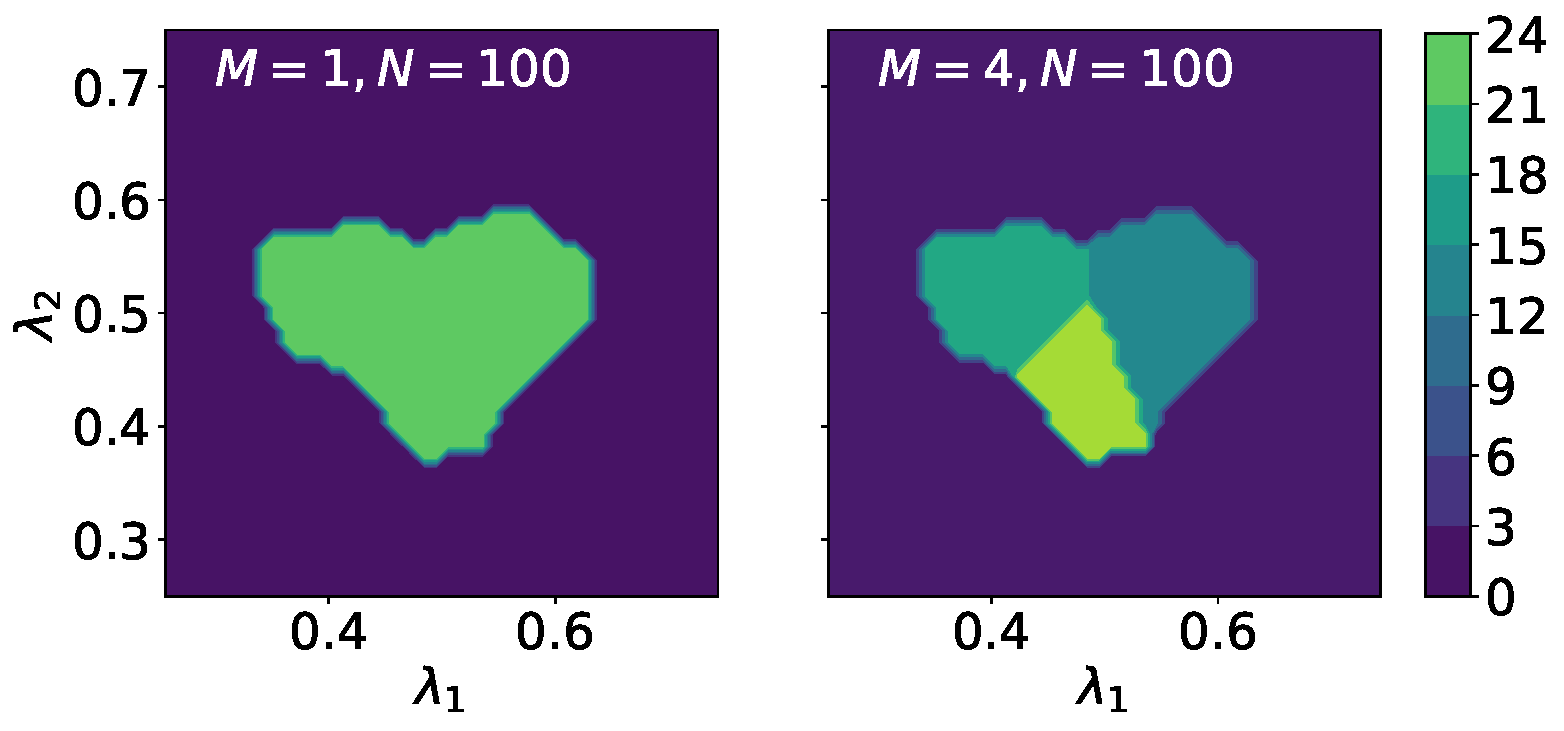
\includegraphics[width=\linewidth]{./examples/identity/set/M1-N100_N100-vs-M4-N100_N100.pdf}
\end{minipage}
\caption{
$\nsamps=100$ were used to discretize $\pspace$ and $\ndiscs=1, 4$ (left/right) were used to discretize $\dspace$.
The latter was chosen to visualize the geometry of describing $\pspace$ with $\pborel$.
}
\label{fig:ex:identity_set_1E2}
\end{figure}

We have chosen a uniform density to describe the uncertainty in our output space.
Any value that is within $0.1$ to the left and right of the reference value \pythoninline{Qref = [0.5, 0.5]} in each dimension is treated as equally likely.
This was done so that using $\ndiscs = 1$ samples to discretize $\dspace$ would fully characterize the characteristic function density representing this uncertainty.
The inverse image of this set is a characteristic function defined on $\pborel$, so errors will exist in particular at the boundaries of the region.

The fundamental challenge with the set-based approach is linked to the geometry of the induced Voronoi-cell tesselation on $\pspace$.
With only $\nsamps = 100$ samples, we see in \ref{fig:ex:identity_set_1E2} that the region (which is supposed to be a square) hardly represents one.
There is ample variation in the shape parameters of the induced sets $\VV_\iparam$ when so few samples are used.
It is possible to ``get lucky'' with the aligning of boundaries between the true target density $\Chi_{[0.4, 0.6]^2}$, but the Figure is representative of the difficulty of using $\nsamps = 100$ random samples to describe a geometry.
With $\nsamps = 1000$, there are usually still significant differences in the symmetric difference of approximated and true supports of the densities.

Below, we demonstrate the use of more samples to resolve the geometry of the desired set.
\begin{figure}[ht]
\begin{minipage}{.975\textwidth}
  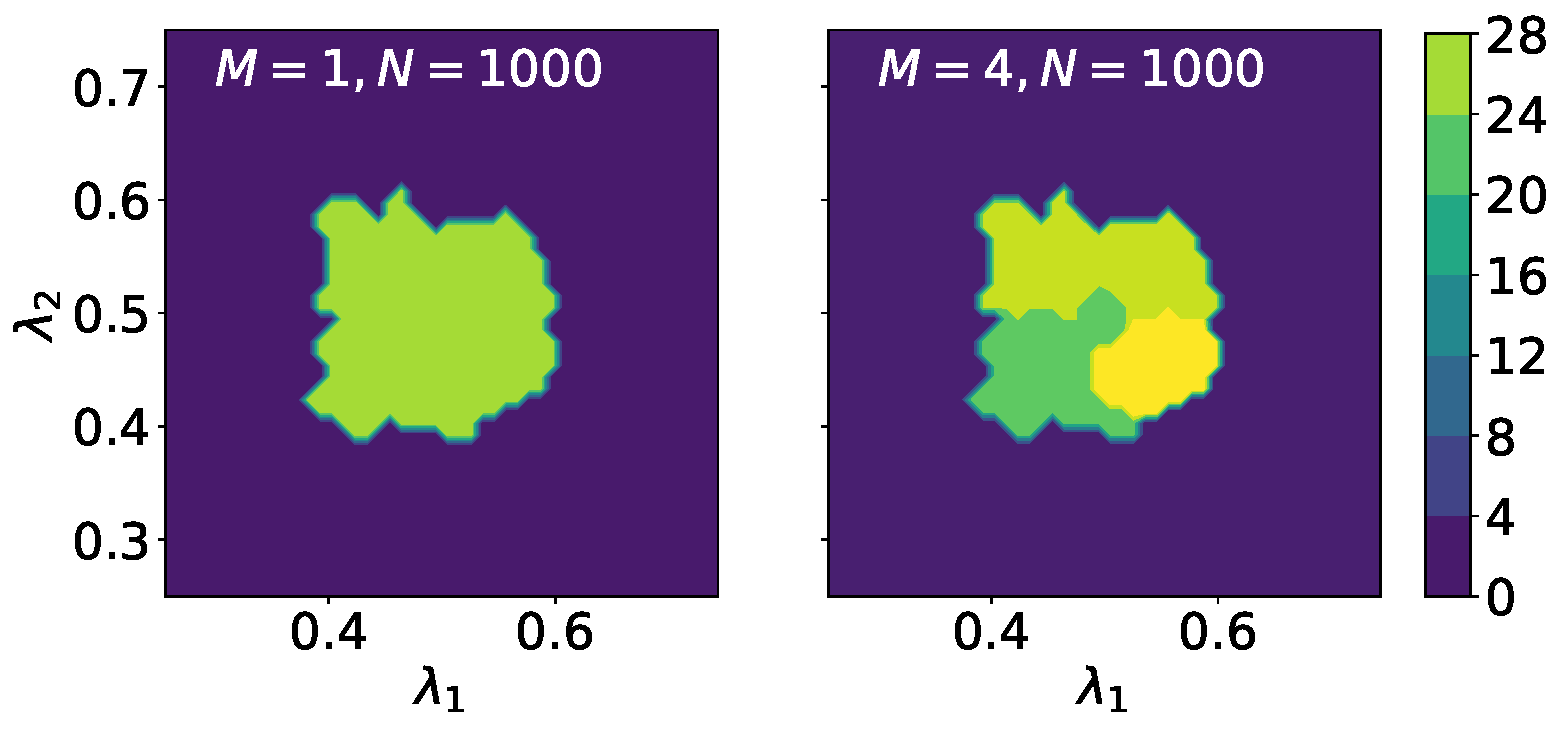
\includegraphics[width=\linewidth]{./examples/identity/set/M1-N1000_N1000-vs-M4-N1000_N1000.pdf}
  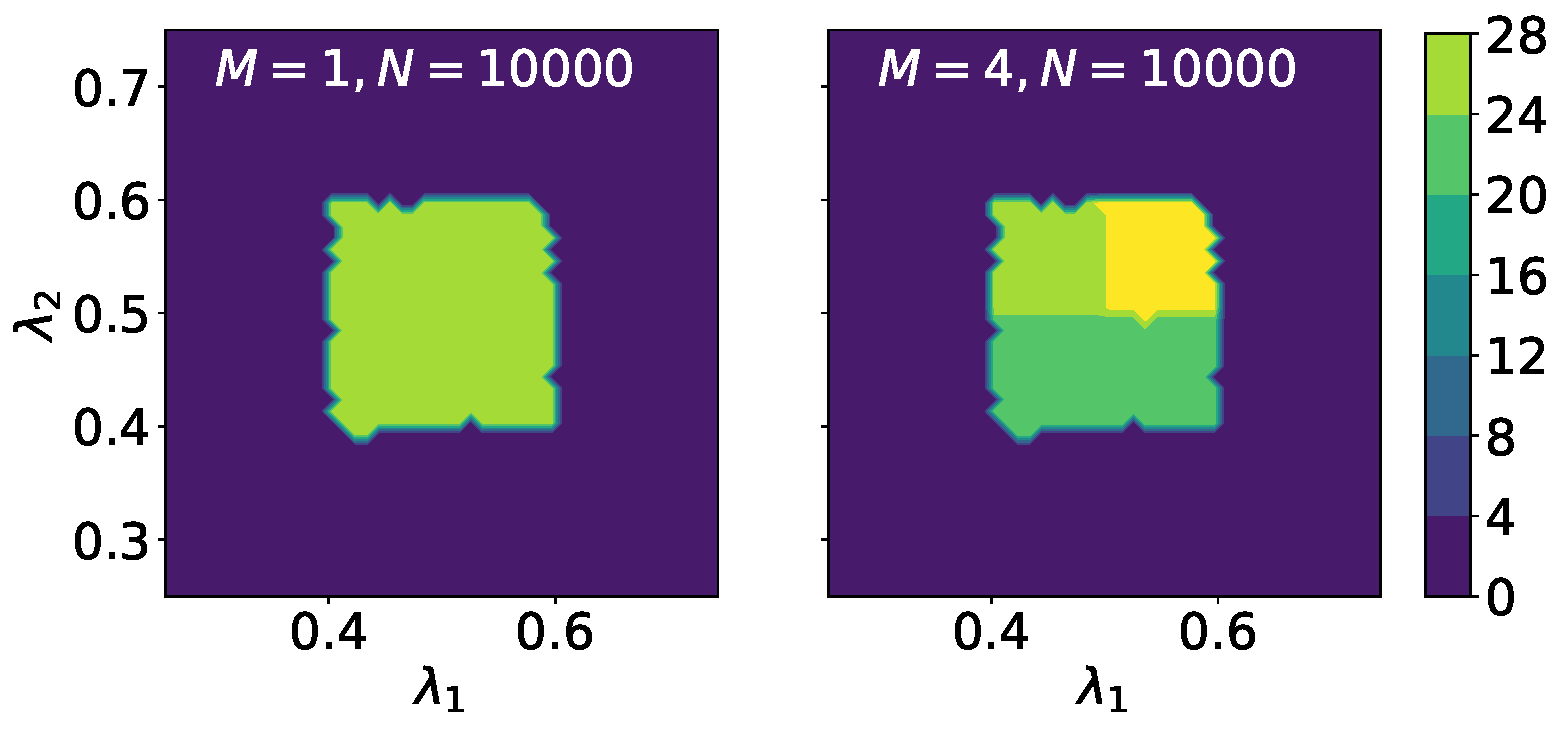
\includegraphics[width=\linewidth]{./examples/identity/set/M1-N10000_N10000-vs-M4-N10000_N10000.pdf}
\end{minipage}
\caption{
(Top):$\nsamps=1,000$ were used to discretize $\pspace$ and $\ndiscs=1, 4$ (left/right) were used to discretize $\dspace$.
(Bottom): The same, except with $\nsamps=10,000$, where we finally begin to see something resembling the correct correct geometry.
}
\label{fig:ex:identity_set_1E3_1E4}
\end{figure}
\FloatBarrier

We remark on the fact that in this particular situation, $\ndiscs = 1$ is a ``correct'' choice for the probability measure chosen, and $\ndiscs = 4$ actually introduces errors.
The reason that the latter solutions have different values inside of the support of $\PPspace$

%\FloatBarrier

%%%%%%%%%%%%%%%%%%%%%%%%%%%%%%%%%%%%%%%%%%%%%%%%%%%%%%%%%%%%%%%%%%%%%%
% \pagebreak
%\section{Sample-Based Inversion for Measures}\label{sec:ch02-sample}

%% Intro
% In [TK - reference] it was shown that an equivalent derivation to the same set-based solution to the SIP presented in \ref{sec:ch02-set} could be achieved with the following form:

\begin{equation}
\dciP
\end{equation}


This equation presents on the left-hand side the solution to the SIP, referred to as the updated measure $\updatedP$, which is equal to a scaling of an initial probabaility measure $\initialP$ by a ratio of observed $\observedP$ to predicted $\predictedP$ measures.
Taking the Radon-Nikodym derivatives of each of the respective terms, we can arrive at a more natural distribution-based description of the solution:

\begin{equation}
\begin{split}
\dci\\
\dciD
\end{split}
\end{equation}

The initial density $\initial$ encodes the information that the ansatz played in \ref{sec:ch02-set}, which is to assign relative probabilities among points which belong to the same equivalence class of solutions.

% \FloatBarrier
%% Numerical Approximation
% \subsection{Numerical Approximation and Analysis}\label{sec:sample-algorithm}

[TK - Algorithm goes here]

picture of pushforward given different number of samples, overview of KDE

% \FloatBarrier
%% Descriptions of Error
% \subsection{Descriptions of Error}\label{sec:sample-error}

[TK - this section below is still a bit rough, but the ideas are starting to get laid out]

The source of approximation error in the sample-based approach comes from a fundamentally different source.
We transfer the burden of responsibility for accurate approximation towards the data space instead of the parameter space.
To estimate a push forward distribution, samples that are drawn from the initial density represent our total model evaluation budget.
For the sample-based approach, it is important to ask: \emph{Is the number of samples still important for accurate approximation?}
We demonstrate that the answer is yes, but the dependence is shifted from the parameter space to the data space, which is often of a lower dimension, which requires less samples to accurately approximate due to the dependence of density approximation on dimension.
We construct a similar triangle inequality as in \ref{sec:set-error}, but the sources of error now bear different interpretations.

We have by repeated application of the triangle inequality that

\begin{equation}
\label{eq:sample-triangleineq}
d(\PP_{\pspace, \ndiscs, \nsamps, h}, \paramP) \leq
\underset{ \text{(E1)} }{\underbrace{d(\PP_{\pspace, \ndiscs, \nsamps, h},\PP_{\pspace, \ndiscs, \nsamps})}} +
\underset{ \text{(E2)} }{\underbrace{d(\PP_{\pspace, \ndiscs, \nsamps}, \PP_{\pspace, \ndiscs}) }}+
\underset{ \text{(E3)} }{\underbrace{d(\PP_{\pspace, \ndiscs}, \paramP) }}.
\end{equation}


Since there is no error in approximating the specification of an observed distribution, the only sources of error are those that arise from inaccurately assigning probability to samples in the denominator of equation \eqref{eq:updated-density} (i.e., approximating the predicted distribution/measure).
The merits of different density approximation methods is beyond the scope of this work, but we provide a brief review of the challenges involved with approximating distributions in high dimensions.
In some sense there is a need to balance the size of the data space and the number of samples available to characterize it.
If model evaluation is cheap, larger data spaces can be constructed to be more informative and have better geometric properties for approximating a solution.
If model evaluations are limited, or perhaps already exhausted, then there may be motivation to pose a one-dimensional problem because it minimizes error in the predicted distribution due to dimension.
We are motivated to minimize the difference in dimension between input output space but as the dimension of the day is best grows, our approximation error at a fixed sample size grow out of proportion.

We summarize some illustrative results for clarification from \cite{Silverman} on the topic of one-dimensional Gaussian density estimation.
The table in \ref{table:silverman} shows the required sample size as a function of dimension required to ensure that the relative mean square error at zero is less than 0.1 (which says nothing of global accuracy).

\begin{figure}
  \begin{tabular}{ l | l }
  \hline \\ Dimensionality & Required Sample Size\\ \hline
  1  & 4\\
  2  & 19\\
  3  & 67\\
  4  & 223\\
  5  & 768\\
  6  & 2 790\\
  7  & 10 700\\
  8  & 43 700\\
  9  & 187 000\\
  10 & 842 000\\ \hline
  \end{tabular}
\caption{Sample size required (accurate to about 3 significant figures) to ensure that the relative mean square error at zero is less than $0.1$, when estimating a standard multivariate normal density using a normal kernel and the window width that minimizes the mean square error at zero.}
\label{table:silverman}
\end{figure}

To achieve this tolerance of 0.1 for a integrated square error $E \int (\hat{f} - f)^2 / \inf f^2$ would require approximately $1.7$ times the samples shown in \ref{table:silverman} for dimensions up to 10 \cite{Silverman}.
The sample sizes required grow even larger for global measures of accuracy, which are fortunately rarely required to achieve in practice due to the nature of $\observed$ assigning probability over only a region of $\predicted$.

% \FloatBarrier
%% Example
% \subsection{Example}\label{sec:sample-example}

We have observed how the set-based approach to solving inverse problems can lead to errors in approximating measures, particularly around the boundaries of the solution set.
The sample-based approach that we summarized above does not rely on Voronoi-cell approximations of contour events, instead assigning probability to random samples drawn from an initial density.

We demonstrate that for estimating a uniform density over a subset of the initial parameter space, the sample-based approach is able to more accurately approximate it at a given sample size.
The reason for this is that the approach has a different source of error, involving estimating to push forward of the initial density.

We are interested in studying how our ability to estimate a uniform density is impacted by the number of samples drawn from the initial density.
We form an inverse problem with the identity map an standard uniform initial densities, with observed densities being uniform over $[0.4, 0.6]^2$, representing a hundred-fold reduction in uncertainty when the problem is solved

We solve the same problem as before but use a uniform initial density in place of a uniform ansatz.
We sample $N=100$, $1,000$ and $10,000$ samples from the initial density and use Gaussian kernel density estimation to approximate the denominator in Eq [TK - eq], and show the resulting updated densities in Figure~\ref{fig:ex:identity_sampling_approx}.

Observe that the support of the updated density matches the solution of the previous inverse problem but is much more accurately approximated.
Gone are the jagged edges that we saw before, replaced by clean squares.
The relative probability is assigned within the support are also more similar to one another, something we demonstrate in Figure~\ref{fig:identity_sampling_conditionals}, which shows conditional densities along the unit directions through the center of the domain.

\begin{figure}[ht]
\begin{minipage}{.975\textwidth}
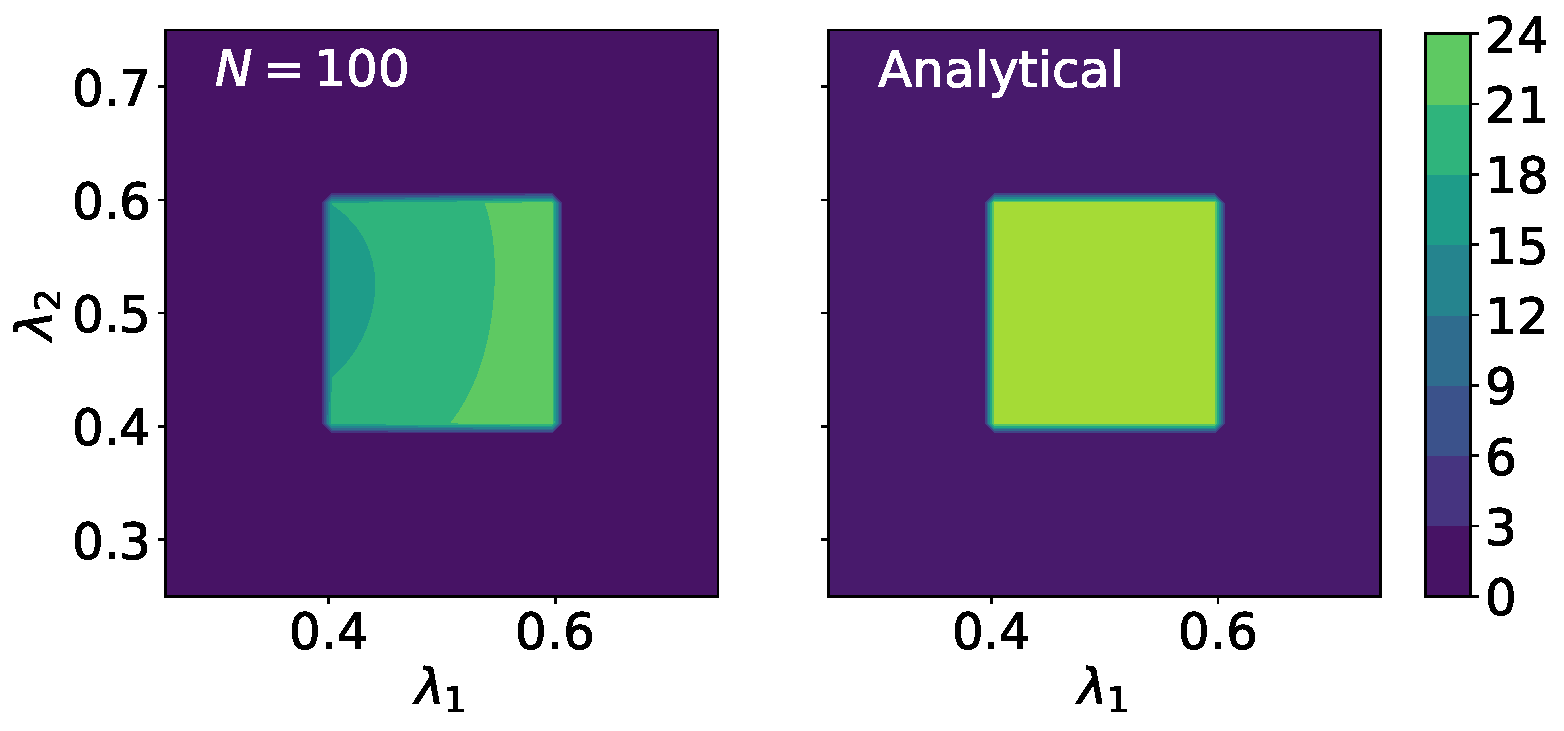
\includegraphics[width=\linewidth]{./examples/identity/samp/N100_N100-vs-Analytical_N100.pdf}
\end{minipage}
\caption{
(Left): $\nsamps=100$ were used to construct the predicted distribution $\predicted$.
(Right): By specifying an analytical $\predicted$, the effect of using $\nsamps$ to approximate a pushforward distribution disappears. The problem can be fully specified in BET without any random sampling.
}
\label{fig:ex:identity_sampling_exact}
\end{figure}

\begin{figure}[ht]
\begin{minipage}{.975\textwidth}
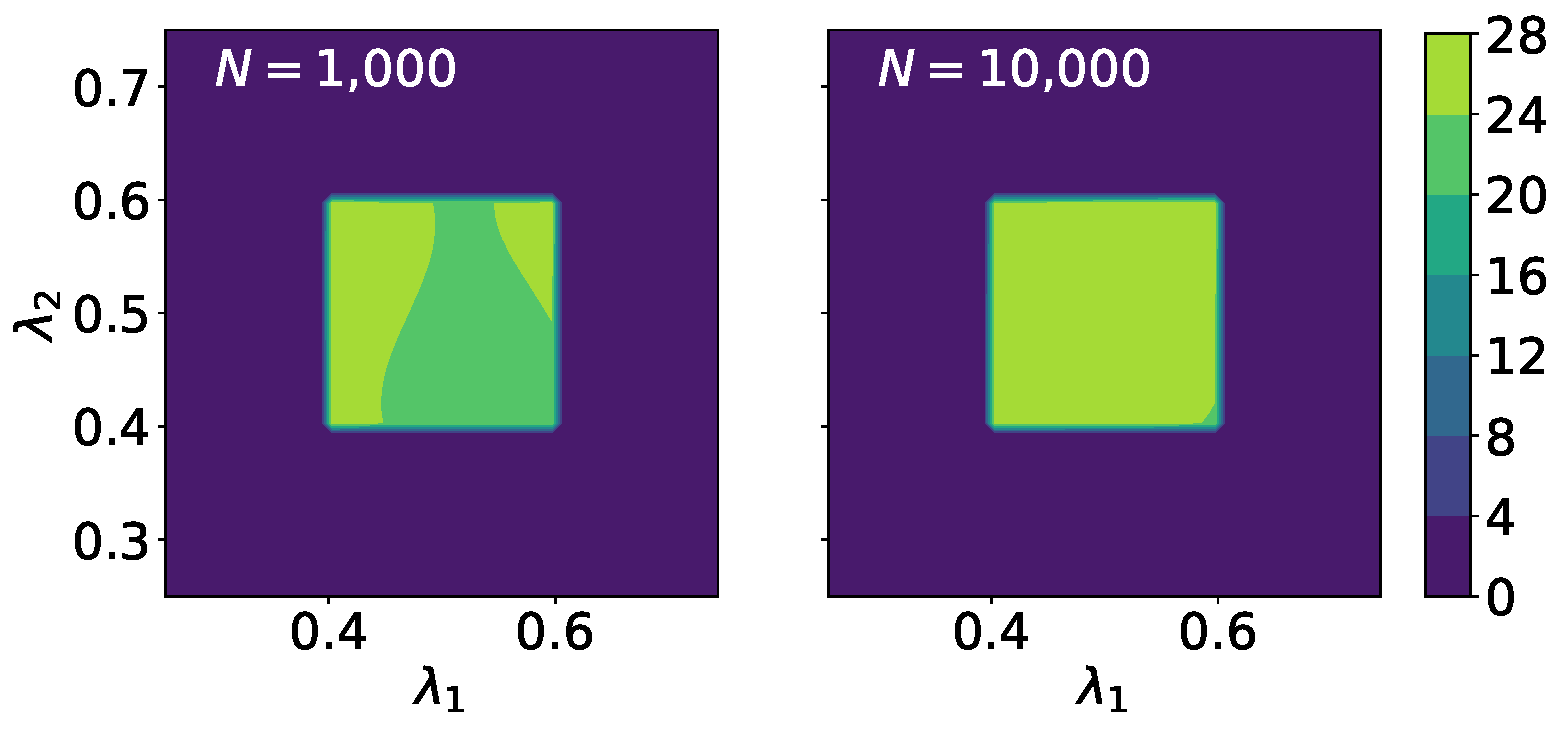
\includegraphics[width=\linewidth]{./examples/identity/samp/N1-000_N1000-vs-N10-000_N10000.pdf}
\end{minipage}
\caption{
$\nsamps=1,000$ (left) and $\nsamps=10,000$(right) were used to construct the predicted distribution $\predicted$.
There is no signficant error in estimating the support of the distribution, only the density approximation itself.
}
\label{fig:ex:identity_sampling_approx}
\end{figure}

\begin{figure}[ht]
\centering
% N = 1E2
\begin{minipage}{.975\textwidth}
		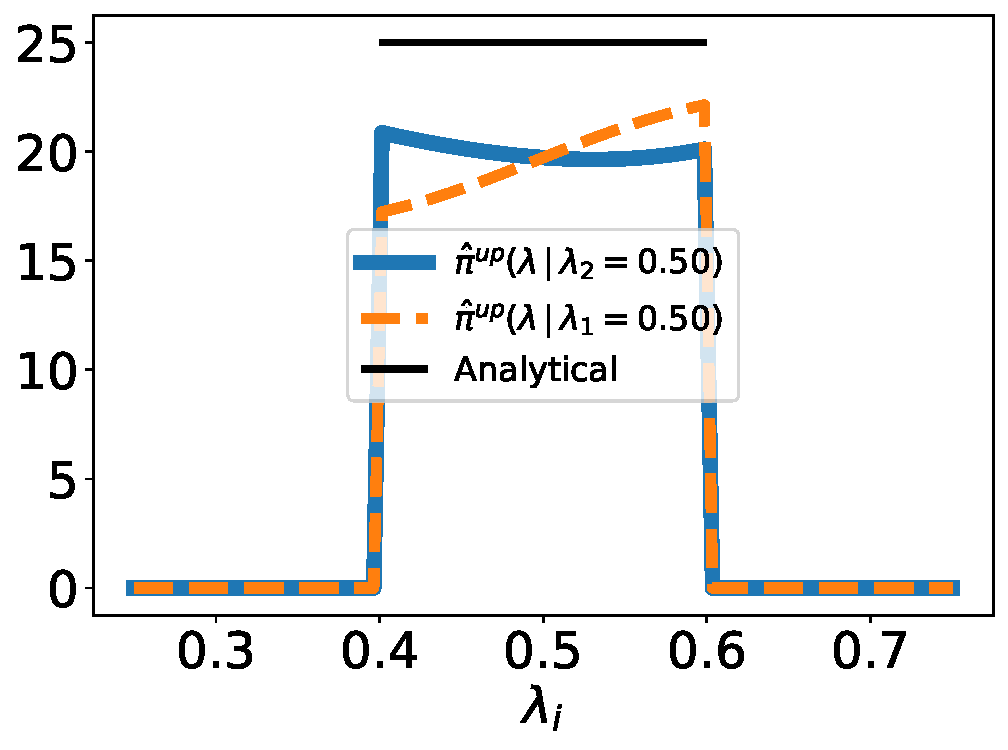
\includegraphics[width=0.5\linewidth]{./examples/identity/samp/identity_1d_conditionals_50E-2_N100_approx.pdf}
    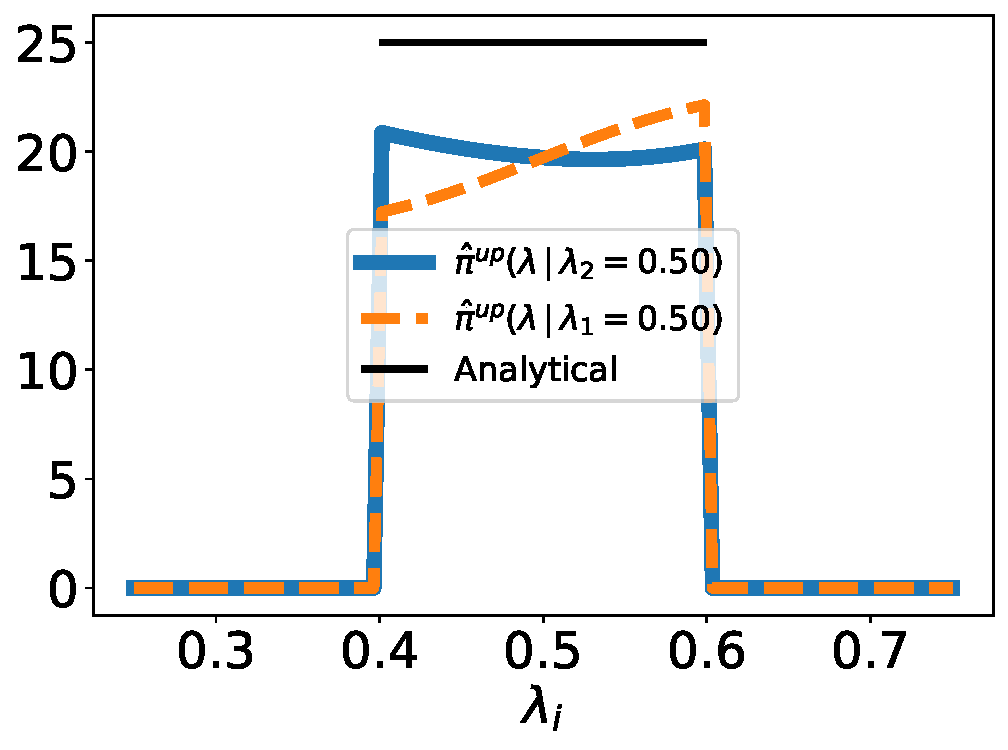
\includegraphics[width=0.5\linewidth]{./examples/identity/samp/identity_1d_conditionals_50E-2_N100_approx.pdf}
\end{minipage}
% N = 1E3
\begin{minipage}{.975\textwidth}
		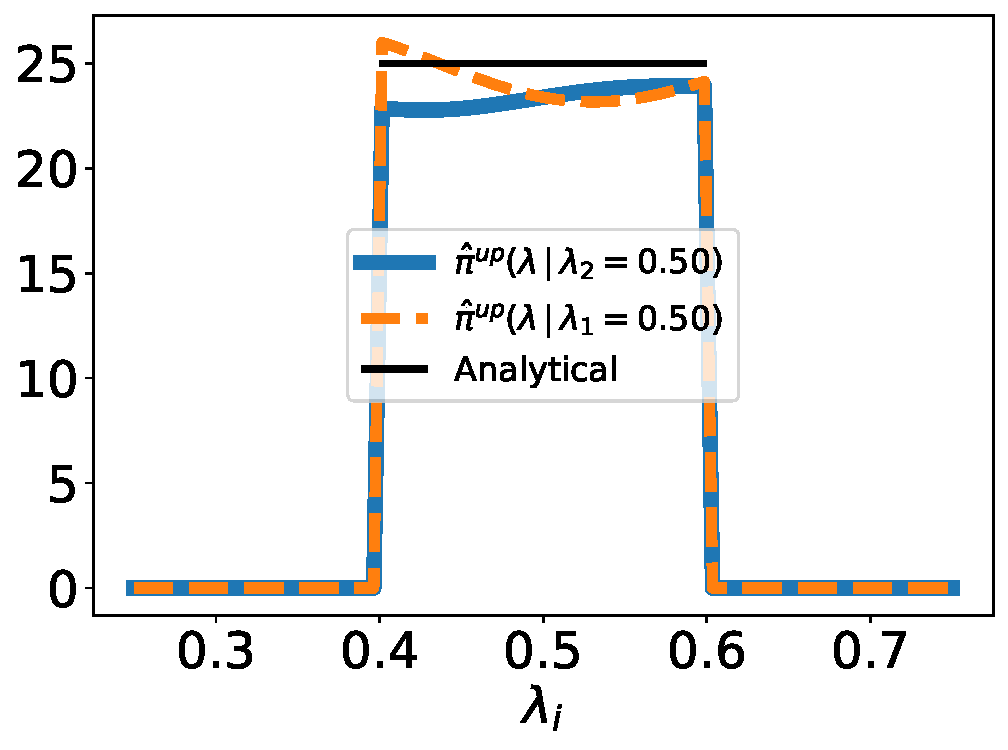
\includegraphics[width=0.5\linewidth]{./examples/identity/samp/identity_1d_conditionals_50E-2_N1000_approx.pdf}
		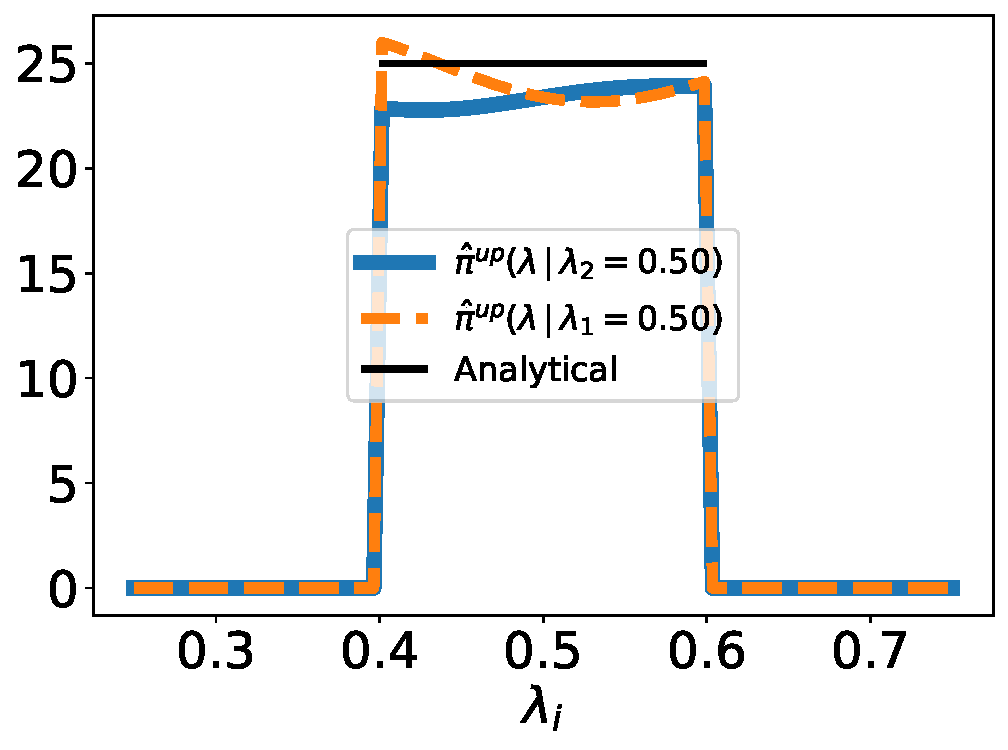
\includegraphics[width=0.5\linewidth]{./examples/identity/samp/identity_1d_conditionals_50E-2_N1000_approx.pdf}
\end{minipage}
% N = 1E4
\begin{minipage}{.975\textwidth}
		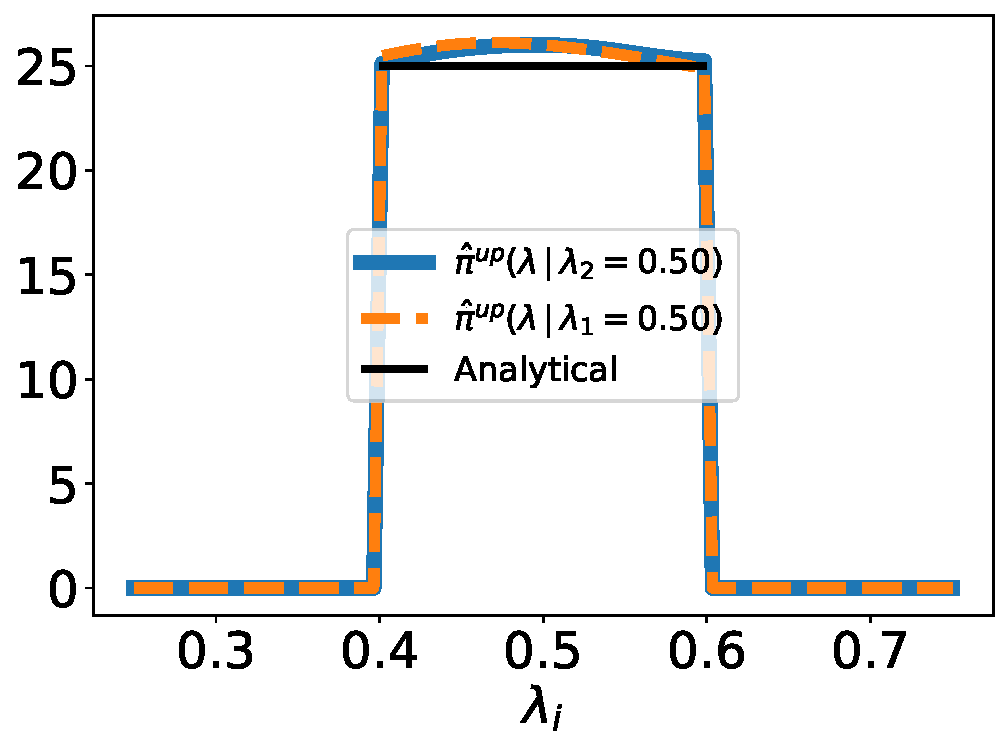
\includegraphics[width=0.5\linewidth]{./examples/identity/samp/identity_1d_conditionals_50E-2_N10000_approx.pdf}
		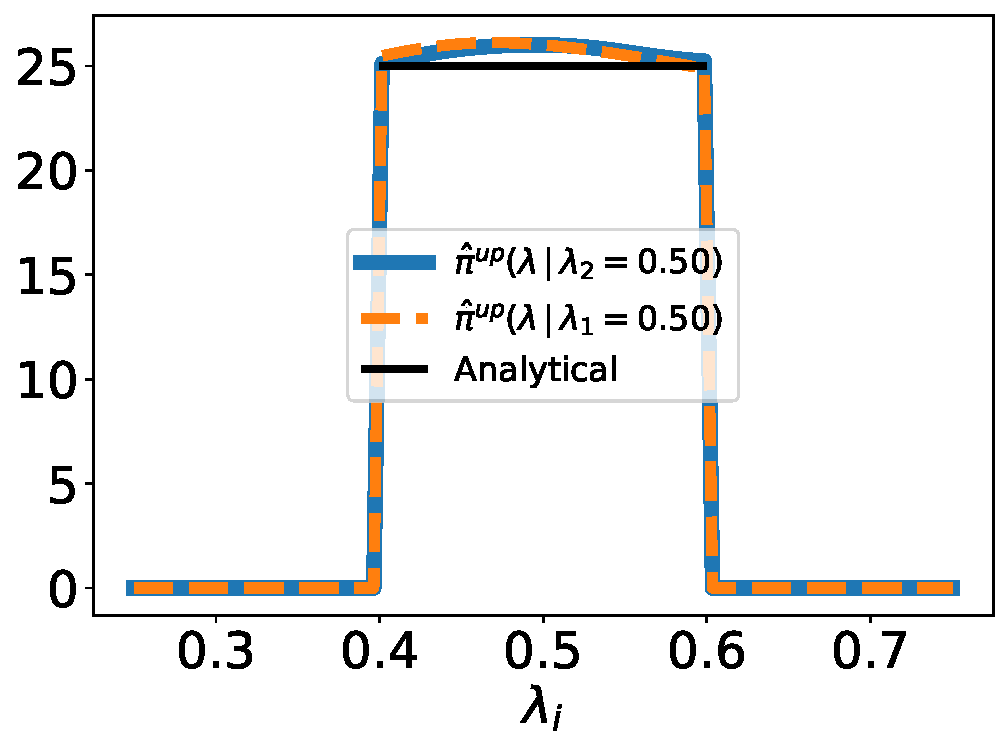
\includegraphics[width=0.5\linewidth]{./examples/identity/samp/identity_1d_conditionals_50E-2_N10000_approx.pdf}
\end{minipage}
\caption{
(Left): $\param_1=0.5$ conditional.
(Right): $\param_2=0.5$ conditional.
(Top to Bottom): Conditional for $\updated$ solutions for  $\nsamps=1E2, 1E3, \text{and} 1E4$ random samples.
}
\label{fig:identity_sampling_conditionals}
\end{figure}

Qualitatively speaking we find that the estimate of the density improve as more samples are used, but at all sample sizes, the support of the density is correctly identified, which we can see by the sharp lines in Fig~\ref{fig:identity_sampling_conditionals} and \ref{fig:ex:identity_sampling_approx}.

The sample-based method trades one source of accuracy for another.
When estimating boundaries of a set which represents an equivalent class of solutions is important, the sample best method provides a compelling alternative to be set based method.

However, we know that this is not without its pitfalls, as density estimation in high dimensions can become prohibitively prone to error.

% \FloatBarrier


%%%%%%%%%%%%%%%%%%%%%%%%%%%%%%%%%%%%%%%%%%%%%%%%%%%%%%%%%%%%%%%%%%%%%%

% \section{Illustrative Examples}\label{sec:ch02-examples}
% In some examples, an analytic, closed-form expression for the QoI map is used.
% In these examples, term (E1) in Eq.~\eqref{eq:set-triangleineq} is identically zero.
% Furthermore, since the probabilities we introduce on $\dspace$ in the numerical results are uniform and our maps linear, the densities can be described analytically with a characteristic function.
% In this event, the solution $\paramP$ to the SIP is given exactly by a change of variables formula and its support can be specified exactly.
% By inverting characteristic functions, the solutions are also be members of this same family of functions if the choice of \emph{ansatz} (or \emph{initial density}) is taken to be uniform over $\pspace$.
% 
% Such simplifications in the examples considered here allow us to study the DCI method for a class of functions for which a solution is readily available, and serves as a requisite testing ground before advancing to more nuanced problem definitions.
% In a sense, these are both ``unit'' (and ``regression'') tests for various aspects of the computational algorithms (and entire algorithms, respectively).
% We present a brief overview of the factors that influence our practical ability to accurately approximate $\paramP$ and $\updated$ using finite sampling.
% 
% For the set-based approach discussed in \ref{sec:ch02-set}, $\ndiscs$ is chosen independent of $\nsamps$ so that (E3) = $d(\PP_{\pspace, \ndiscs}, \paramP)$ from \ref{sec:set-error} is sufficiently small or eliminated entirely.
% In other words, the decision about how to discretize the uncertainty in $\dspace$ is made a priori to cater to some problem specifications.
% We choose to impose uniform distributions on $\dspace$ so that the set-valued analog to $\observed$ is perfectly described with $\ndiscs=1$.
% Elimintating this variable allows for a better comparison between the set- and sample-based approaches.
% Therefore, we focus our attention on the source of error introduced by the primary contribution of error in Eq.~\eqref{eq:set-triangleineq}:  discretizing the parameter space, which is represented by the term (E2) = $d(\PP_{\pspace, \ndiscs, \nsamps}, \PP_{\pspace, \ndiscs})$.
% The number of samples fundamentally limits the characterization of events due to the resulting simple-function approximation of the density $d\paramP / d\pmeas$, which we compare to $\updated$ from the sample-based approach.
% Since there is no error introduced from discretizing $\pspace$ in the sample-based approach from \ref{sec:ch02-sample}, the primary contribution of error in this approach comes from approximating the push-forward density in situations where an analytical $\predicted$ is not known.
% 
% \FloatBarrier
% 
\subsection{Exponential Decay}\label{ex:decay-set-sample}

To demonstrate the qualitative differences in the solutions provided by the set-- and sample--based methods for a nonlinear problem, we consider an exponential decay problem with uncertain decay rate and initial condition (which are paired to form the 2-D vector $\param$):
$$
\begin{cases}
  \frac{\partial u}{\partial t} & = \param_1 u(t), \\
  u(0) &= \param_2.
\end{cases}
$$

The solution is described by
\begin{equation}
  u(t;\param) = u_0\exp(\param_1 t), \; u_0 = \param_2 ,
\end{equation}

and a nominal value of $\param = 0.5$ is used to simulate the system.
We take a single observation at $t=0.5$s and assume a uniform density with interval length $0.2$ centered at $u(1,0.5)$ to represent the uncertainty in the measurement equipment.
We assume a uniform ansatz / initial density over the unit domain.
We use $N=50$ parameter samples to establish a coarse solution in Figure~\ref{fig:heatrod-sol-ex1}.


\begin{figure}
\begin{minipage}{.475\textwidth}
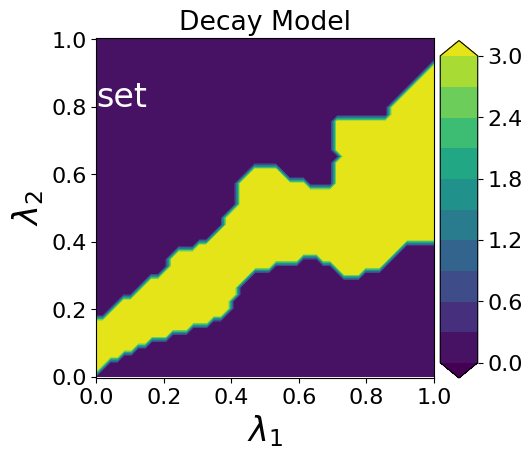
\includegraphics[width=\linewidth]{examples/fig_decay_q1/DecayModel--set_N50_em.png}
\end{minipage}
\begin{minipage}{.475\textwidth}
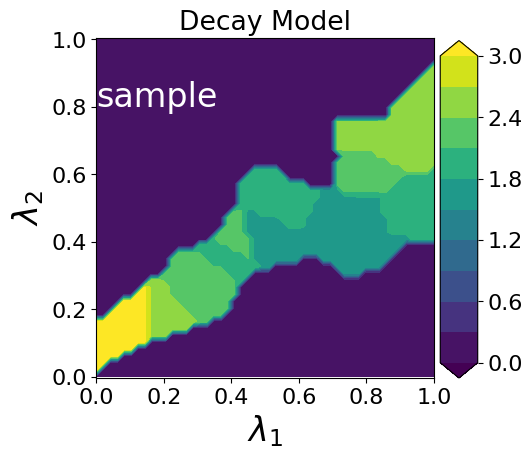
\includegraphics[width=\linewidth]{examples/fig_decay_q1/DecayModel--sample_N50_mc.png}
\end{minipage}
\caption{Observation taken at $t=1$s. The inverse image of the reference measure for set-based (left) and sample-based (right) solutions for $\nsamps=50$ parameter samples.}
\label{fig:heatrod-sol-ex1}
\end{figure}

The decay rate $\param_1$ shows little reduction in uncertainty overall.
If one were to look at marginals of the components of $\param$, it would not appear as if much was learned.
However, the relationship \emph{between} these two quantities has very certainly been elucidated by the solution of the inverse problem.
Where once $\pspace$ was a rectangular region, the set of possible parameters has been reduced to a diagonal band.
The sample-based approach, especially at this low sample size (density estimation in 2-D at $50$ samples is a stretch), has some visible downsides.
It does not capture the equivalence--class nature of the solution set the way the set--valued one does, which benefits from using $\ndiscs=1$ (aligning with the choice of uniform observed density).


We address what would occur had we been able to observe earlier in time at $t=0.5$ by showing the associated solutions under the same experimental conditions in \ref{fig:heatrod-sol-ex2}.
There is a marked reduction in uncertainty, as several regions of $\pspace$ have been ruled out from consideration.


\begin{figure}
\begin{minipage}{.475\textwidth}
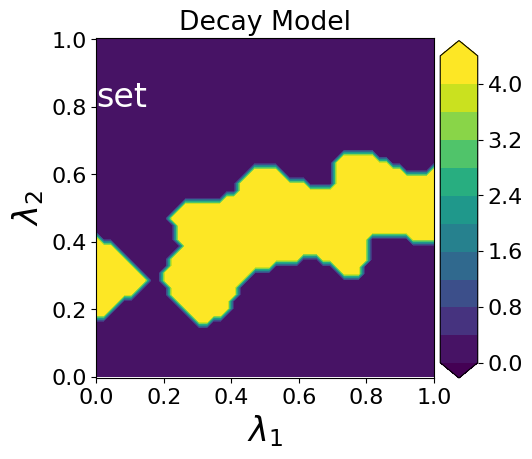
\includegraphics[width=\linewidth]{examples/fig_decay_q2/DecayModel--set_N50_em.png}
\end{minipage}
\begin{minipage}{.475\textwidth}
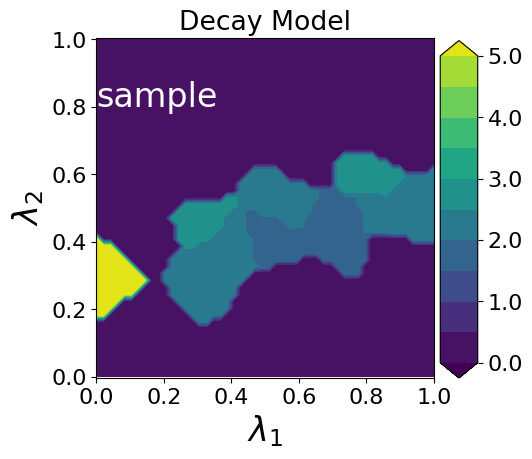
\includegraphics[width=\linewidth]{examples/fig_decay_q2/DecayModel--sample_N50_mc.png}
\end{minipage}
\caption{Observation taken at $t=0.5$s. The inverse image of the reference measure for set-based (left) and sample-based (right) solutions for $\nsamps=50$ parameter samples.}
\label{fig:heatrod-sol-ex2}
\end{figure}


Observing earlier in time helps especially in reducing the (marginal) values for the initial condition $\param_2$, while the rate $\param_1$ is still to some degree able to take any values in its original domain.
Both solution types suffer from discretization error, as evidenced by the break in the contour structure.
By comparison to \ref{fig:heatrod-sol-ex1}, there is more more confidence in the solution (represented by the reduced support of the image).

However, at $\nsamps=50$, the sample--based approach struggles to assign uniform probability to different contour events.
This may suggest that in situations with very limited model evaluation budget and set-valued solutions involving uniform uncertainties in measurements, the set-valued approach may serve a useful purpose.

% 
% \FloatBarrier
% \subsection{1D Heat Rod}\label{ex:heat-set-sample}

Consider the one-dimensional heat equation with homogeneous Neumann boundary conditions on the unit interval:

\begin{equation}
\begin{split}
\rho c \frac{\partial T}{\partial t} = \nabla \cdot ( \kappa \nabla T) + f(x), \quad & x\in (0,1), t\in (0,1) \\
f(x) = A e^\frac{- (x-0.5)^2}{w} \Chi_{[0,0.5]}(t)
\end{split}
\end{equation}
\emph{Alternative setup: }

\begin{equation}
\begin{cases}
\rho c \frac{\partial T}{\partial t} = \nabla \cdot ( \kappa \nabla T) + f(x,t), & \text{if } x\in \Omega \\
\frac{\partial T}{\partial \vec{n}} = 0 & \text{if } x\in \partial \Omega
\end{cases}
\end{equation}
where $\Omega = (0,1)\times (0,1)$ is the space-time interior and $f(x,t) = A e^\frac{- (x-0.5)^2}{w} \Chi_{[0,0.5]}(t)$.

Here, we interpret the following problem as heating the middle of an infinitesimally thin unit-length rod for half a second with the heat-source modeled by a Gaussian curve with amplitude $A=50$ and variance of $w=0.05$.
The rod is subdivided in two, and each half has an uncertain thermal diffusivity $\kappa \in [0.01, 0.2]$.
This yields a two-dimensional parameter space $\param = (\param_1, \param_2) \in [0.01, 0.2]\times [0.01, 0.2]$, where $\param_1$ represents the thermal diffusion on the left-half and $\param_2$ is the $\kappa$ for the right half.

\begin{figure}[h]
\begin{minipage}{.475\textwidth}
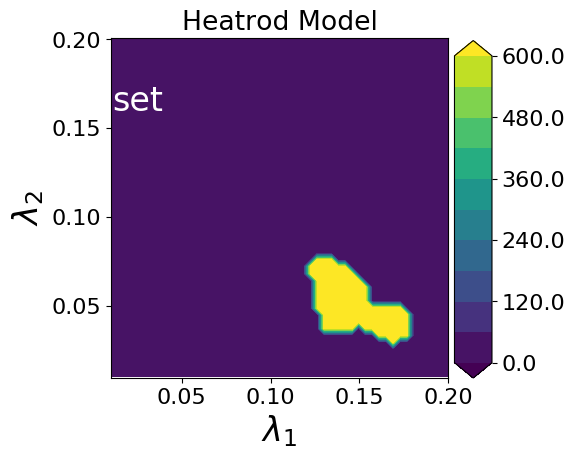
\includegraphics[width=\linewidth]{examples/fig_heatrod_q1/HeatrodModel--set_N50_em.png}
\end{minipage}
\begin{minipage}{.475\textwidth}
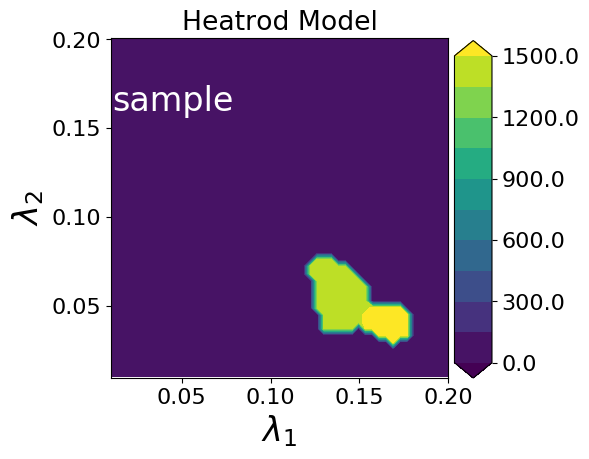
\includegraphics[width=\linewidth]{examples/fig_heatrod_q1/HeatrodModel--sample_N50_mc.png}
\end{minipage}
\caption{The inverse image of the reference measure for set-based (left) and sample-based (right) solutions for $N=50$ parameter samples.}
\label{fig:heatrod-sol-ex}
\end{figure}


\chapter{\uppercase{Computational Framework} \label{chapter:02}}

\section{Towards a Reproducible Thesis}\label{sec:reproducibility}

\subsection{Motivations}\label{sec:motivations}
In some respects, the practice of writing software has diverged from the motivations of an academic researcher.
The latter seeks to generate new knowledge and may write a set of example scripts/programs to demonstrate some novel idea or method.
By contrast, the motivations of a software engineer are related to resiliency.
Not only must they ensure the code works as expected given a myriad of ways users may interact with it, but it is necessary to write the code in a manner compatible with maintaining it into the future.
Much of the work of writing ``good software'' is concerned with writing appropriate documentation to express the intended usage and logic underlying architectural decisions.
There are many ways to write a functioning program to demonstrate a proof-of-concept, but creating something that is \emph{user-friendly}, guaranteed to be free of mistakes, and scales across different computational environments/resources requires an entirely different approach.

Decisions made early in the software design cycle have lasting impacts on future features and functionality.
Rigor is added to libraries through the writing of \emph{unit tests}, and use of \emph{continous integration} ensures that the download and installation process is predictable and reproducible.
Code that only runs on the author's computer is impractical, since any thorough critique requires independent verification.
Without proper context and architecture, new ideas that are implemented in programs are unlikely to be adopted.


This thesis is concerned not only with a demonstration of novel mathematical content\---showcasing new ways to make inferences from noisy data in a novel Data-Consistent framework\---it also serves to document the process of ensuring that the work is \textbf{fully reproducible}.
In mathematics, reproducibility is ensured through the use of proofs, which motivate the original work presented here.
However, as the title of this thesis suggests, much of the focus is actually on the computational implementation of the novel research into Data Consistent Inversion, studying the impact of using computers to perform the task of making conclusions based on data.
Mathematics is implemented on computers through software.
We are therefore concerned with ensuring the expected functionality of that software, which aligns with our training as mathematicians; we care deeply about making sure things are rigorous.

In short, we want to make sure that theory aligns with practice, and that both live up to high standards of intellectual scrutiny.
Every computational result, illustrative figure, table, plot, etc. presented in this thesis is associated with the scripts that generate them, and are included in the  repository for this document [TK - cite].
It is written in \LaTeX~(which is itself a programming language), and presents its own software dependencies in addition to those required to run the scripts to generate the images and tables.
To address this concern, we leverage \emph{Travis}, a continuous integration service [TK-cite], to ensure that all figures can be generated and the \LaTeX\, document compiles into a PDF.

The same care is taken to ensure the reproducibility of all numerical results based on software.
An \emph{image} that contains a fully pre-built Linux software environment within which one can compile the thesis and run the code is available through the Docker Cloud registry [TK -cite].
The latter enables the ability to generate this thesis document in its entirety on any software platform that supports Docker (Windows, MacOS, Linux).
A cloud service called Binder [ TK - cite mybinder.org] allows one-click deployments in any web-browser, removing the need for any installation whatsoever for anyone wanting to reproduce the contents of this document.



\section{Software Contributions}\label{sec:software-contributions}

As discussed in \ref{sec:motivations}, the entirety of the mathematical content presented has been incorporated into freely available open-source software, including this document.
The novel mathematical developments that have gone into this work are all reflected in various modules and sub-modules as part of the BET Python package.
This software suite follows a number of industry best-practices for code-coverage (\ref{sec:code-coverage}) and continuous integration (\ref{sec:continuous-integration}), i.e. the code is well-tested (\ref{sec:unit-testing}).

A significant effort in the writing of this thesis involved learning about the art and practice of modern (open-source) software development.
The author spent most of 2019 bringing the software in-line with the latest developments in Data-Consistent Inversion.


%%%%%%%%%%%

\subsection{Software Design and Architecture}\label{sec:architecture}

Having learned a lot about software reproducibility along the way, the author made the decision to treat this thesis as a software project in its own right.
Every example, figure, table, and plot is generated by a combination of Python and Shell scripts contained inside of a public Github repository (www.github.com/mathematicalmichael/thesis).

By hosting this work on Github, corrections can be submitted as Issues, and the document can serve as a reference point for a thorough introduction on the topic of Data-Consistent Inversion.
All the requisite \LaTeX~dependencies are contained in {\tt apt.txt}, and a Jupyterlab environment usable by Binder (which can compile the document and run every example) is configured in the {\tt binder/} directory of the repository (on the binder branch).

Special care is taken to ensure that every script is at least minimally documented.
When appropriate, functions and classes are used in such a way that the same file generates several examples in this thesis.
The parameters required for the variations are passed as optional arguments, and Shell scripts + makefiles containing the exact syntax to generate each figure are included.
The makefiles are particularly useful in that they track dependencies, so if changes are made to a plotting script, running {\tt make} will re-create only the figures which leverage that changed code.


We illustrate with a specific example: to visually demonstrate the implicitly-defined sets of nearest-neighbors in two-dimensional unit domain, we rely on Voronoi-cell diagrams.
One Python file (\bashinline{images/voronoi_unit_domain.py}) contains the methods required to draw a single figure; however, there are many occasions where variation on a plot may be necessary (for example, labels, different line widths).
To accommodate the need for different variations of similar plots, we utilize the argument-parsing package \pythoninline{argparse}, part of the Python standard library, to enable command-line positional and optional arguments \footnote{We equip each function with default values so that the syntax \bashinline{python example.py} without any additional arguments will work, but specific examples rely on optional arguments to be passed accordingly.}.
We include associated (wrapper) files with descriptive names, such as \bashinline{images/make_voronoi_diagrams.sh} that repeatedly call the relevant Python file(s) and passes arguments (such as {\tt num} for ``number of samples'').
We refer the inquisitive reader to  Figure~\ref{fig:voronoi_cells} or \ref{fig:voronoi_issues} to see the Voronoi-cell diagrams generated by the following script\footnote{A \LaTeX macro has been written to allow for Python and Bash files to be displayed contextually to avoid the need to update them in two places. What is shown in the body/appendix of this work is an embedded and stylized version of the exact script that was executed to generate figures.}:

\bashexternal{images/make_voronoi_diagrams.sh}


These wrappers are called by other shell scripts which are each responsible for generating figures in different sections or specific models.
This builds something akin to a ``tool chain'' or a ``pipeline,'' a series of calls to hierarchies of scripts in order to generate the pictorial and tabular content in this work.

%%%%%%%%%%%
\subsubsection{Software Dependencies and Docker}\label{sec:docker}
[TK - brief intro to images, containers]
We document the process of how the containers which were used to generate all the results here (the {\tt bin/} directory of this thesis contains the relevant shell scripts), are generated by including the Dockerfiles for them.
This static snapshot allows us to be assured our results can be recreated on x86 architecture (theoretically in perpetuity).
The author also published versions of the relevant images compiled on ARM, and has recreated all figures on a Raspberry Pi as validation.
However, at the time of writing there exists a set of dependencies not yet implemented in an arm-based Dockerfile.
The scientific computing software (largely developed by collaborations among researchers at the national laboratories) FeNiCS, was compiled from source on ARM, as a proof-of-concept.
Generating a docker image which builds the software from source on ARM is a to-do for the author, and can already be theoretically brute-forced by copying over the requisite built-files from the host operating system\footnote{As a stopgap measure for ARM-support, the entire RaspberryPi has been backed up to an image and published online, so that all the dependencies can be resolved by switching microSD cards.}.
FeNiCS is available through conda but only on x86, and no ARM-based docker images are provided to be leveraged.


%%%%%%%%%%%
\subsubsection{Testing}\label{sec:unit-testing}
The aforementioned \emph{unit tests} provide a framework for guaranteeing the behavior of programs or individual methods when instructions are followed.
\emph{Functional tests} encompass more complicated behavior, stringing together several methods/modules to ensure code runs as its author intended, and are usually included when referring to unit testing.
``How to write a test'' is a question that depends highly on the particular functionality, but the premise is always the same.

[TK - maybe show a really basic example of a set/get method and the test for that?]

%%%%%%%%%%%

\subsubsection{Code Coverage}\label{sec:code-coverage}

Code coverage refers to the proportion of lines of code that were run during the process of testing (consisting of unit and functional tests).
The goal is not necessarily to achieve 100\% coverage, but rather to make sure that the most crucial use-cases are checked.
Generally speaking, coverage in the 75-85\% range is industry-standard.

[TK - flesh out a bit more, talk about Codecov, the specific service we use, how it won't be used for the scripts in this thesis].

%%%%%%%%%%%

\subsubsection{Continuous Integration}\label{sec:continuous-integration}

These outer-level scripts that call others are leveraged by continuous-integration (CI) services (Travis, Github Actions), that run a series of commands on behalf of the user, automating the process of testing functionality.
The familiarity with this technology was introduced as a consequence of working on BET \cite{pyBET}, the software library that originally implemented the set-based approach discussed in \ref{sec:ch02-set}.
The use of CI in BET is similar to that of many software packages written in Python; unit tests are run in some framework (\pythoninline{nose} for BET at first, eventually migrated to \pythoninline{pytest} at the author's insistence), and a successful run triggers a webhook that communicates with the software repository host (Github) to validate changes. Github receives messages from the CI service and shows a visual indicator of the status of the work done.

Github Actions came out [TK - date] during the final year of writing this thesis, and provided a convenient way to orchestrate and check on the status of continuous-integration and deployment

\subsubsection{Continuous Deployment to DockerHub and PyPi}
Give an intro to CD principles. Relevant here because the {\tt mud} Python library which implements the analytical expressions presented here and is a shared library for many of the examples, particularly in Chapter~\ref{chapter:mud}.
This library leverages all of the aforementioned principles and components, and additionally automatically publishes to the PyPi registry, allowing anyone to {\tt pip install mud} to resolve \emph{most} of the dependencies of novel contributions presented here.
A similar effort is underway for CD in BET, though the version(s) used here have already been published ({\tt pip install bet}).
Even as changes are made after this thesis is published, readers of this work can rest assured that the results are still reproducible because Github Actions validates all of it on a weekly schedule.
As soon as reproducibility problems surface, the author will be notified so they can be addressed, and the latest build status of the project is visible to the public.

\subsection{Background and Motivation}
The open-source software package BET was developed actively from 2012-2015 under grant [TK grant-NSF+DOE].
It was originally written in Python 2.7 and is currently administered by the Computational Hydrology Group at the University of Texas: Austin through their UT-CHG GitHub group [TK - cite Github].
The initial purpose of this open-source software package was to implement the methods first described in [TK - cite BET papers] for the description and solution of stochastic inverse problems summarized in Section~\ref{sec:ch02-set}.
In the intervening years since its original publication in [TK - date of first release, cite Github], the BET package has seen two major releases and the incorporation of several sub-modules (e.g. the functions in {\tt sensitivity} implement much of the original research performed by Dr. Walsh [TK - cite Scott]).


\subsection{Upgrades, Updates, and Features}
Since the last major release [TK - cite latest release], the Python community announced the end of long-term support for Python 2 [TK - cite announcement].
Several of the dependencies in BET have been actively developed in Python 3 with no updates to the Python 2 analogs, which necessitated an upgrade to allow the package to be a usable contribution to open source software.
The work summarized in Section~\ref{sec:ch02-sample} was implemented in Python 3 independently by the author through the release of the ConsistentBayes package.
Since that code was used for many of the preliminary results for this work, it made very little sense to re-implement them in Python 2 for BET given the recent trends in community development.
With funding made available through the NSF [TK - cite grant], the opportunity to upgrade BET to Python 3 allowed the library to avoid falling into disuse by relying on an unsupported language.


\subsubsection{Version 2.1.0}
The upgrade to Python 3.4+ began in January 2019 as a first step to incorporate the new sample-based method into BET.
It was completed in late February.
Major (minor? version? TK) release 2.1.0 [TK - put in release] was designed to provide backwards-compatibility with the Python 2.7 version.
Future installations (starting in 2020) will not limit the versions of some core dependencies in order to accommodate backwards-compatibility with Python 2 (e.g. {\tt numpy}, {\tt scipy}), since this would likely downgrade previously installed software for end-users.


\subsubsection{Version 2.2.0}
Several releases of BET (after the upgrade to Python 3 in v2.1.0), incorporated developments that will be discussed herein.
[TK - i have no recollection what the significance of this was]

\subsubsection{Version 2.2.1}
Major bugfix for parallel testing allowed tests to pass for more than 2 processors.
For some tests, this involved changing the setup parameters to ensure the problem was large enough to break up onto up to 8 processors.
For others, significant changes had to be made to structure to allow for proper saving and loading of files in parallel.


\subsubsection{Version 2.3.0}
This release incorporated the sampling-based approach discussed in Section~\ref{sec:ch02-sample}.
However, it never made it to the master branch of the project due to architectural changes in BET.
It was used for generating many of the results in this thesis initially by pointing to {\tt install\_bet.sh} which pulled the specific branch, but eventually this was swapped for Version 3.0.

\subsubsection{Version 3.0}
This version implemented the sample-based approach by the introduction of new sub-classes.
It broke backwards-compatibility with much of the code written for this work.
[TK - point to the github PR that eventually upgrades the examples (hopefully including ones for the master's. I figure it's one or two night's work, but very low priority since I am using docker to ensure that everything can be reproduced. In fact, it's actually a testament to git + docker that I can point to code in the past and recreate the results.)]

\subsection{Examples in BET}
Basic plotting functionality of BET is demonstrated in iPython notebooks [TK - some kind of citation here], which have seen an exponential growth rate on GitHub, and can be edited by the end-user to work with different plotting library versions and backends.
These notebooks were originally created to reflect the example suite in BET (which were {\tt .py} files), but later they were migrated into a separate repository BET-examples to allow for better organization.
In the new framework, each notebook functions as an independent example.
Several of these notebooks were adapted from the example code in this thesis repository.


[TK - for ch4 purposes...]
Talk about the BET module that computes metrics.
Discuss testing, show sample of usage (disconnected from skewness, high-level).

\FloatBarrier

\FloatBarrier
% \chapter{\uppercase{Impact of Output Quantities on Accuracy} \label{chapter:03}}

\section{Skewness and Information Content}
Here, we motivate the reduction of a quantity called \emph{skewness} in pursuit of optimizing the geometry of set-valued solutions to stochastic inverse problems with respect to their ability to be well-approximated by Monte-Carlo integration. 
However, the results hold for any attempt to approximate densities defined on sets induced by random samples, and thus may be of interest to the larger research community. 

We demonstrate that the number of samples required to approximate densities using uniform i.i.d.~sampling is proportional to the skewness of the map used for inversion, though the convergence rate of the algorithm used to solve the stochastic inverse problem is unaffected. 



\subsection{Skewness and Accuracy}\label{subsec:skewness}
In \cite{BGE+15}, the concept of skewness in a QoI map $\qoi$ was introduced, quantified, and related to the accuracy in solving the SIP with a finite number of samples.
Essentially, skewness is a geometric property that describes how the right angles in generalized rectangles belonging to $\dborel$ are transformed by $\qoi^{-1}$. 
An a priori analysis demonstrated that the number of samples from a {\em regular uniform grid} in $\pspace$ required to approximate the $\PP_\pspace$-measure of $\qoi^{-1}(E)$ to a desired level of accuracy was proportional to the skewness of $\qoi$ raised to the ($d-1$) power where $d$ is the dimension of $\dspace$.
This is a version of the so-called curse-of-dimension.
Since the numerical solution of the SIP relies fundamentally on the approximation of such $\qoi^{-1}(E)$, it was assumed that skewness impacted the probability measure computed using Algorithm~\ref{alg:inv_density} in a similar way.

Skewness was explored further in \cite{BPW17} in the context of optimal experimental design.
There, an additional geometric property of $\qoi$ related to the {\em precision} in the solution of the associated SIP was introduced and quantified. 
Under the same assumption that skewness impacted accuracy of the numerical solution to the SIP, a multi-criteria optimization problem was formulated and solved to determine a $\qoi\in\qspace$ that balanced accuracy and precision in the SIP solution.

Since no previous study has considered the numerical convergence rates of Algorithm~\ref{alg:inv_density}, the impact of skewness on such rates is unclear.
Moreover, it is not clear that skewness causes errors to pollute the entire numerical solution of the SIP since local approximation errors in the $\PP_\pspace$-measure of contour events have a tendency to cancel out over $\pspace$. 
This is the primary focus of the numerical results in Section~\ref{sec:results}. 
Here, for completeness, we define skewness below and refer the interested reader to \cite{BGE+15, BPW17} for more details.


\begin{defn}
For any $\qoi\in\qspace$, $\param \in \pspace$, and a specified row vector $\bf{j}_k$ of the Jacobian $J_{\param, Q}$, we define
\begin{equation}
S_Q(J_{\param,Q}, \bf{j}_k) := \frac{\abs{\bf{j}_k} }{\abs{\bf{j}_k^\perp}}.
\label{eq:skewness}
\end{equation}

We define the \textbf{local skewness} of a map $\qoi$ at a point $\param$ as 
\begin{equation}
S_Q(\param) = \max_{1\leq k \leq d} S_Q(J_{\param,Q}, \bf{j}_k).
\label{eq:localskewness}
\end{equation}
\end{defn}

\begin{defn}
The \textbf{average} \emph{(or \textbf{expected})} \textbf{skewness} is defined as
\begin{equation}
\overline{S_Q} = \frac{1}{\mu_{\pspace}(\pspace)} \int_\pspace S_Q (\param) \, d\mu_{\pspace}
\label{eq:avgskew}
\end{equation}
\end{defn}

In \cite{BPW17}, it was shown that $S_Q(\param)$ can be efficiently computed using a singular value decomposition of the Jacobian $J_{\param,Q}$. 
In general, we approximate $\overline{S_Q}$ with Monte-Carlo approximations.


%%%% discussion of convergence 

Second, and perhaps most importantly, since the spaces $\pspace$ we are considering are generally bounded and finite, the Hellinger metric metrizes weak convergence (see Thm. 6 in \cite{GS02}).
The latter property is of notable importance because the QoI maps we study are indeed (component-wise) functionals on the space of model inputs $\pspace$. 
Thus, convergence of a sequence of probability measures under the Hellinger metric implies that the QoI's will also converge component-wise in $\RR$. 
In other words, convergence in the Hellinger metric implies the convergence of the sampled QoI map to the exact QoI map since the map is a linear functional of the probability measure. 
In other words, if $\PP_{\pspace,M,N,h}$ converges to either $\PP_{\pspace,M,N}$, $\PP_{\pspace,M}$, or $P_\pspace$ using the Hellinger metric, this implies that the error converged to zero in the numerically computed $Q(\param^{(j)})$.
Thus, convergence in the Hellinger metric implies, in a sense, convergence of the numerical method used to construct the QoI map. 
Furthermore, recall that weak convergence $P_n \to P$ is defined to mean 
\[
\int P_n f \to \int Pf
\]
for bounded Lipschitz functions $f$. 
Taking $f = \Chi_A$, this leads to the following implication:  
\[
\PP_{\pspace, M, N} \to P_\pspace \implies \PP_{\pspace, M, N} (A) \to P_\pspace (A) \quad \forall{A\in\pborel}.
\]
%provided we rigorously define $\P\PP_{\pspace, M, N}$ to measure sets in $\BB_\pspace$, which we proceed to do in the following section\footnote{\bf{I know this is clumsy, but I'm not exactly sure how to phrase this correctly, because it almost seems like this would be true for all $A\in\pspace$ instead. I suppose the omission of the differential operator above is intentionally vague to gloss over this detail. Can we sharpen this up?}}
It is a combination of computational ease of implementation and theoretical implications that motivates the choice of the Hellinger distance as the metric used in the numerical results of Section \ref{sec:results}.



\
\section{Accuracy of Set-Based Inversion}

%%%%%%%%%%%%%% discretization discussion, software contribution in later section



The measures computed from Algorithm~\ref{alg:inv_density} are defined on a set of samples $S = \set{\param^{(j)}}_{j=1}^{N}$ which implicitly define a Voronoi-cell partition $\set{\VV^{(j)}}_{j=1}^{N}$ of the parameter space $\pspace$. 
We let $\BB_{\pspace, N}$ denote the \emph{computational algebra} generated by $\set{\VV^{(j)}}_{j=1}^{N}$, i.e., using standard measure theory notation, 
$$
	\BB_{\pspace,N} = \sigma\left(\set{\VV^{(j)}}_{j=1}^{N}\right).
$$
Clearly, $\BB_{\pspace, N}\subset \BB_\pspace$ and the events $A\in B_{\pspace, N}$ represent the $A\in\BB_\pspace$ for which we can ``easily'' compute probabilities and make inferences.
While Algorithm~\ref{alg:inv_density} ultimately defines a probability measure implicitly on $(\pspace,\BB_\pspace)$, computationally this is almost never done and the measures are only interrogated on the computational algebra associated with the set of samples. 

Different sets $S_k = \set{\param{(i)}}_{i=1}^{N_k}$, where the $\param^{(i)}$'s and $N_k$'s may be completely different for each $k$, will lead to different measures computed from Algorithm~\ref{alg:inv_density}. 
Each $S_k$ induces a computational algebra which we index using the notation $\BB_{k}$ for simplicity, where it is understood that $\BB_k = \BB_{\pspace, N_k}$. 

This poses an immediate problem with respect to a computational approach to computing $d_H$: how do we compare measures $\PP_{\pspace, M, N_1}$ and $\PP_{\pspace, M, N_2}$ which may be defined on completely different computational algebras (even if $N_1=N_2$)?
See Figure~\ref{fig:voronoi_issues} for an illustration of such a scenario.

\begin{figure}[h]
\centering
	\begin{minipage}{.4875\textwidth}
		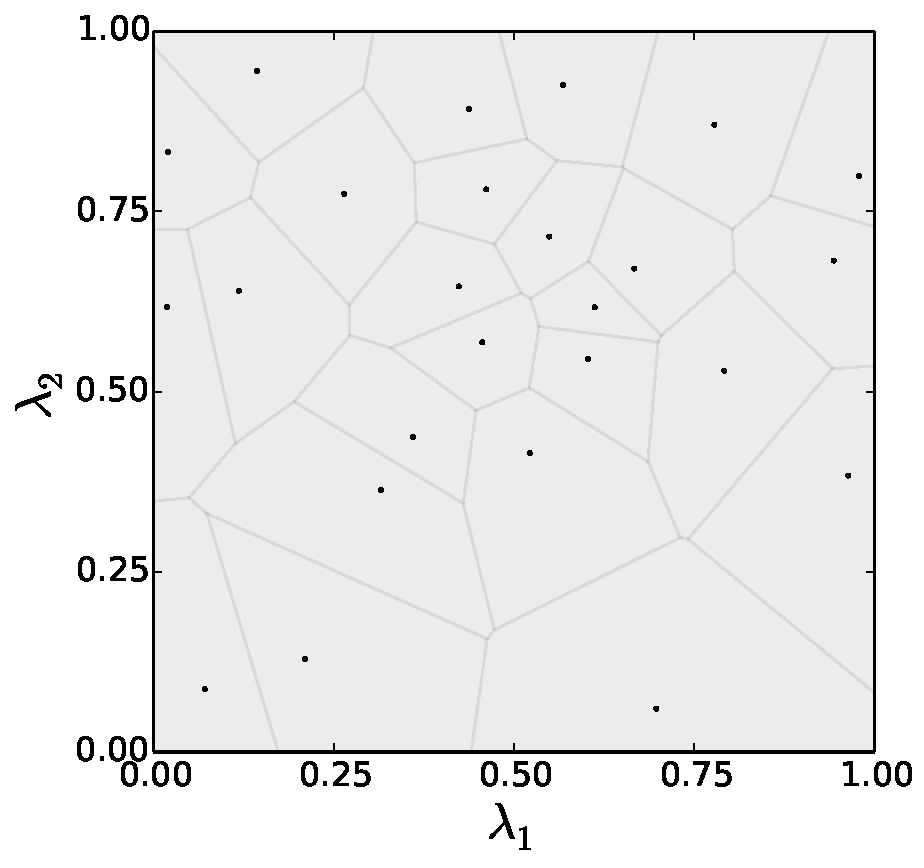
\includegraphics[width=\linewidth]{./images/voronoi_diagram_N25_r0}
	\end{minipage}
%	\begin{minipage}{.3\textwidth}
%		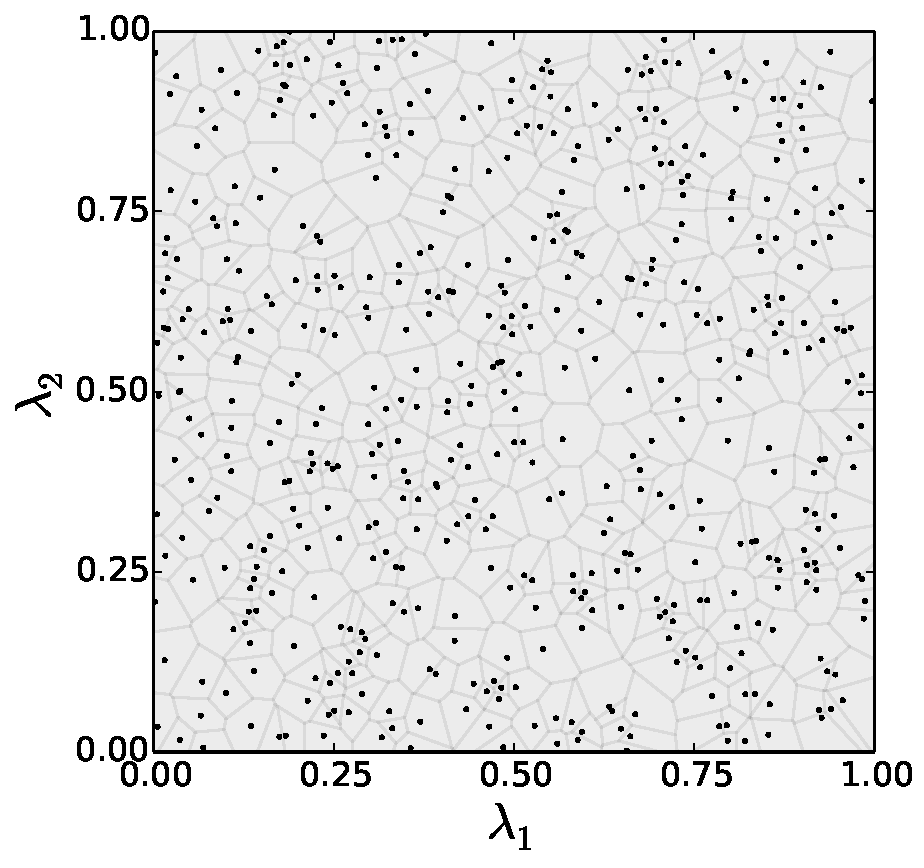
\includegraphics[width=\linewidth]{./images/voronoi_diagram_N500_r50}
%	\end{minipage}
		\begin{minipage}{.4875\textwidth}
		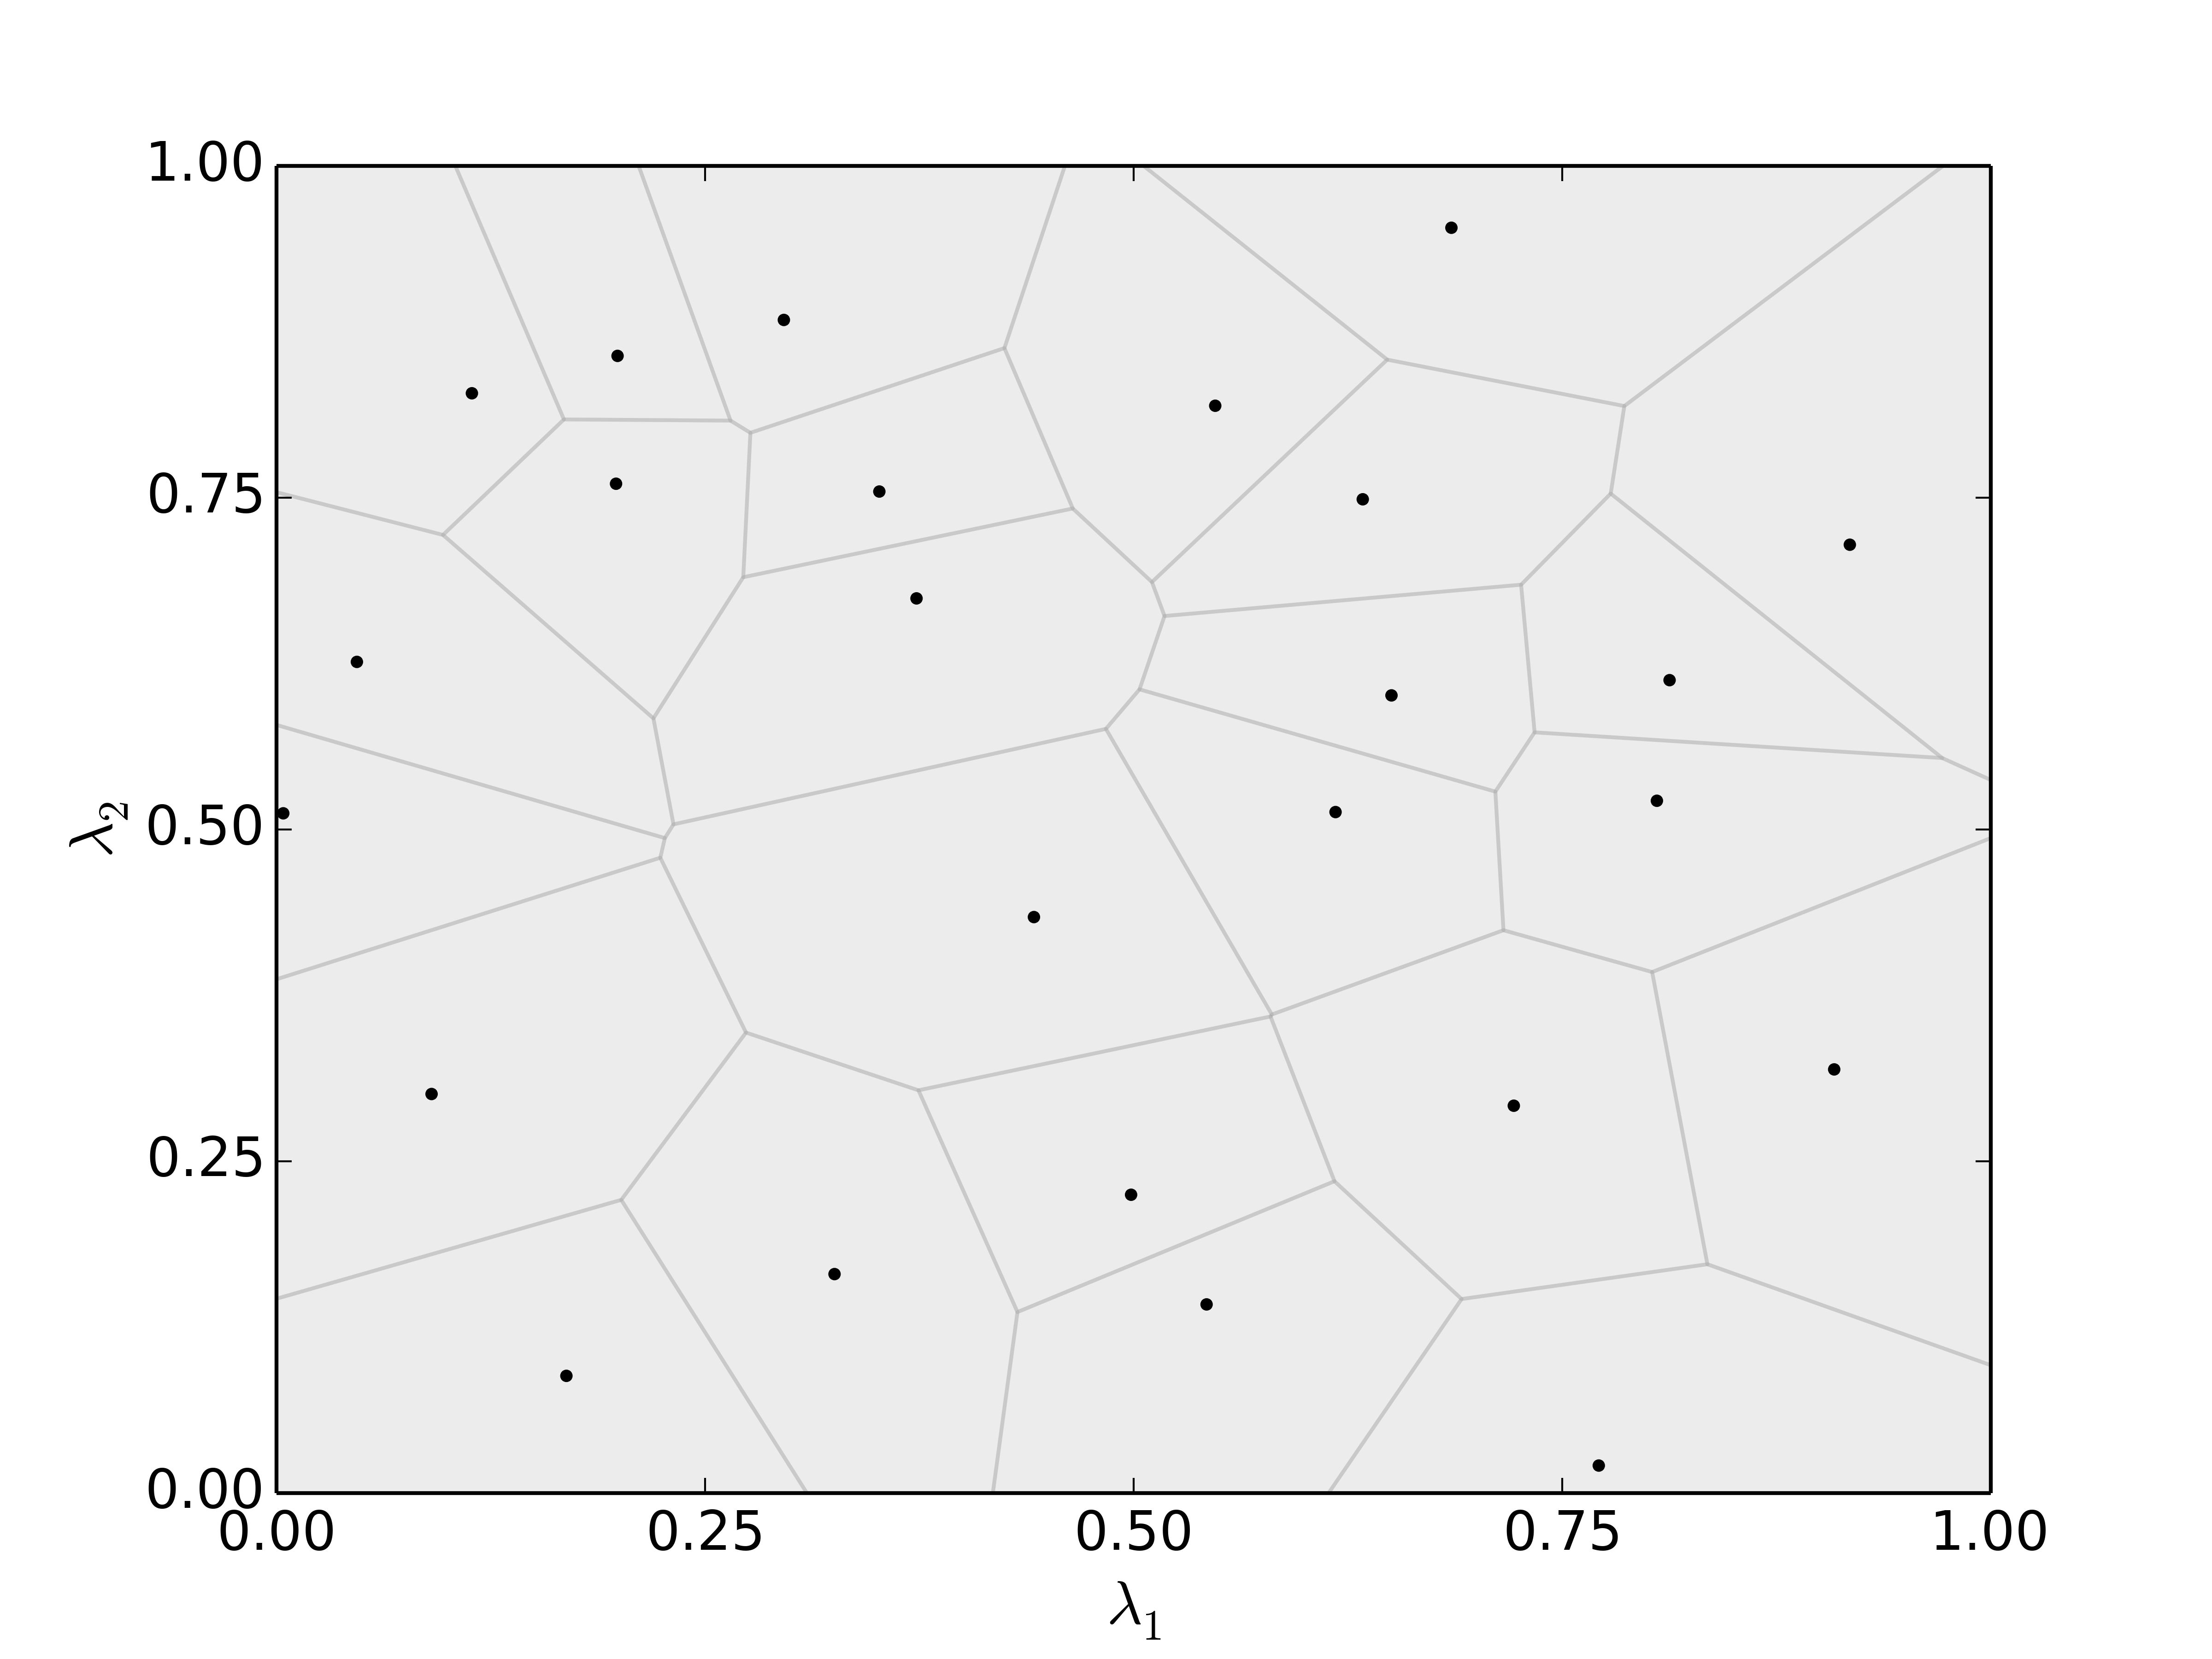
\includegraphics[width=\linewidth]{./images/voronoi_diagram_N25_r10}
	\end{minipage}
\caption{
Two different Voronoi partitions induced by $N_1 = N_2 = 25 $ uniform i.i.d.~random samples. 
%Center:  A possibly over-resolved reference generated using $N_2 = 500$. We want the ability to seamlessly compare measures defined on any such two discretizations as inputs to a metric.
}
\label{fig:voronoi_issues}
\end{figure}


The proof of the following Lemma describes how to ``computationally extend'' {\em any} probability measure defined on a computational algebra to a full $\sa$ $\BB$, which we exploit in Algorithm~\ref{alg:hellinger_disc}.
\begin{lem}
\label{lem:measuresets}
Let $\mu$ be a measure on $(\pspace, \BB_\pspace)$, $\set{\VV^{(j)}}_{j=1}^{N}$ be a partition of $\pspace$, and $\BB_{\pspace, N}$ the computational algebra generated by $\set{\VV^{(j)}}_{j=1}^{N}$. 
Assume $\mu (\VV^{(j)}) > 0 \; \forall \; j=1,\hdots, N$. 
Then, there exists a probability measure $\eta$ on $(\pspace, \BB_\pspace)$ such that $\eta(A) = \eta_N(A) \; \forall \; A\in\BB_{\pspace, N}$. 
\end{lem}
In the proof below, we use $\eta_N$ and $\mu$ to construct a type of ``discrete'' Radon-Nikodym derivative of $\eta$. 
This is motivated by the formal structure of solutions given by Algorithm~\ref{alg:inv_density}.
\begin{proof}
Let
\begin{equation}\label{eq:finiteradon}
f_N (\param) = \sum_{j=1}^{N} \frac{\eta_N (\VV^{(j)}) }{\mu (\VV^{(j)})} \Chi_{\VV^{(j)}} (\param).
\end{equation}
Then, for any $A\in\BB_\pspace$, define
\begin{equation}\label{eq:approxmeasure}
\eta (A) = \int_A f_N (\param) \, d\mu.
\end{equation}
We verify that $\eta$ is a probability measure on $(\pspace, \BB_\pspace)$ and that $\eta(A) = \eta_N(A) \; \forall \; A\in\BB_{\pspace, N}$ below:
\begin{itemize}
\item[(i)][Positive]
Let $A\in \BB_{\pspace}$.
\begin{equation*}
\begin{split}
\eta (A) &= \int_A f_N (\param) \, d\mu \\
&=  \int \Chi_A \sum_{j=1}^{N} \frac{\eta_N (\VV^{(j)}) }{\mu (\VV^{(j)})} \Chi_{\VV^{(j)}} (\param) \, d\mu \\
&= \sum_{j=1}^{N} \left ( \frac{\eta_N (\VV^{(j)}) }{\mu (\VV^{(j)})} \int \Chi_{A\cap\VV^{(j)}} (\param) \, d\mu \right ) \\
&= \sum_{j=1}^{N} \left ( \frac{\eta_N (\VV^{(j)}) }{\mu (\VV^{(j)})} \mu\left (A\cap\VV^{(j)}\right ) \right ) \geq 0
\end{split}
\end{equation*}

\item[(ii)][Definite]
\begin{equation*}
\eta (\nullset) = \int_\nullset f_N (\param) \, d\mu =\int \Chi_\nullset f_N (\param) \, d\mu = \mu(\nullset) = 0
\end{equation*}

\item[(iii)][Countably Additive]
Let $\set{A_k}_{k=1}^{\infty} \subset \BB_{\pspace}$.
\begin{equation*}
\begin{split}
\eta (\cup_k A_k) &= \int_{\cup_k A_k} f_N (\param) \, d\mu 
= \int \Chi_{\cup_k A_k} f_N (\param) \, d\mu \\
&= \int \left( \sum_k \Chi_{A_k} \right ) f_N (\param) \, d\mu
=   \sum_k \int \Chi_{A_k} f_N (\param) \, d\mu \\
&=   \sum_k \int_{A_k} f_N (\param) \, d\mu = \sum_k \eta(A_k)
\end{split}
\end{equation*}


\noindent Finally, let $A\in\BB_{\pspace, N}\subset \BB_\pspace$. 
Then there exists some $j^* \in \set{1,2, \cdots, N}$ such that $\VV^{(j^*)} = A$. 
We have that
\begin{equation*}
\begin{split}
\eta (A) &= \int_A f_N (\param) \, d\mu
=  \int \sum_{j=1}^{N} \left ( \frac{\eta_N (\VV^{(j)}) }{\mu (\VV^{(j)})} \Chi_{\VV^{(j)}}\right ) \Chi_{\VV^{(j^*)}} \, d\mu \\
&= \int \frac{\eta_N (\VV^{(j^*)}) }{\mu (\VV^{(j^*)})} \Chi_{\VV^{(j^*)}} \, d\mu
= \frac{\eta_N (\VV^{(j^*)}) }{\mu (\VV^{(j^*)})} \mu (\VV^{(j^*)}) \\
&= \eta_N (\VV^{(j^*)}) = \eta_N (A). 
\end{split}
\end{equation*}

\end{itemize}
\end{proof}

We note that in practice, $\Chi_{\VV^{(j)}} (\param)$ requires the use of nearest-neighbor computations, but otherwise evaluation of Eq.~\eqref{eq:finiteradon} is straightforward to compute.

\begin{algorithm}
\DontPrintSemicolon
\caption{Hellinger Discretization}
\label{alg:hellinger_disc}
Let $(\pspace, B_{\pspace, N_1}, \eta_{N_1} )$ and $(\pspace, B_{\pspace, N_2}, \eta_{N_2} )$ be given.\\
 
Construct $f_{N_1}$ and $f_{N_2}$ and corresponding $\eta_1, \eta_2$ using Eq.~\eqref{eq:finiteradon} and Eq.~\eqref{eq:approxmeasure}, respectively.

Use Monte Carlo sampling to approximate
$$ d^2_H(\eta_1, \eta_2) = \int_\pspace \sqrt{f_{N_1}(\param}) - \sqrt{f_{N_2}(\param)} \, d\mu $$.
\end{algorithm}

Since we now have a way to extend probability measures defined on $(\pspace, \BB_{\pspace, N})$ to  probability measure on $(\pspace, \BB_{\pspace})$, we can use simple Monte-Carlo approximation schemes to the Hellinger distance between two probability measures defined on two separate computational algebras. 
This is demonstrated in Algorithm~\ref{alg:hellinger_disc}.


\
\section{Accuracy of Sample-Based Inversion}

How does the new approach compare? What role does the KDE play in the error?
Focus on linear problems. One or two examples (perhaps use that skew-map with 1 and 2 and 4).

\
\section{Software Contributions}

Talk about the BET module that computes metrics.
Discuss testing, show sample of usage (disconnected from skewness, high-level).

\
\section{Numerical Results and Analysis}

Pick an ODE problem and show how the results look like (assimilating as many data points as inputs, if using time-series model). 

Our goal in this section is to provide a set of examples that demonstrate these two approaches, their ``solutions.''
Exponential Decay, uncertain initial condition and rate. Fix two measurement times. No OED discussion.

Show visualization of solution on voronoi-mesh vs. 2D density. 

This is going to set up the stage nicely.
What if we had more measurements to incorporate? Discuss how the distributions we imposed as our observed were kind of a little disingenuous since they were based on single measurements. Well, rather, they represent the answer to a different question.


\FloatBarrier

% \chapter{\uppercase{Impact of Output Quantities on Accuracy} \label{chapter:03}}

Here, we motivate the reduction of a quantity called \emph{skewness} in pursuit of optimizing the geometry of set-valued solutions to stochastic inverse problems with respect to their ability to be well-approximated by Monte-Carlo integration.
However, the results hold for any attempt to approximate densities defined on sets induced by random samples, and thus may be of interest to the larger research community.

We demonstrate that the number of samples required to approximate densities using uniform i.i.d.~sampling is proportional to the skewness of the map used for inversion, though the convergence rate of the algorithm used to solve the stochastic inverse problem is unaffected.
We focus on the accuracy of the density/measure, since this is what solves our SIP.
The updated solution can be used for point estimation, or used holistically for prediction under uncertainty.
Regardless of the context for solving the SIP, it is important to address the sources of approximation error that pollute the observation-consistent framework.

%%%%%

\section{Set-Based Inversion for Measures}\label{sec:set-based}
% Intro
To properly summarize the set-based solution, we define several measure/probability spaces and refer to the schematic given in Figure \ref{fig:scheme} in order to illustrate the steps and spaces required in the formulation and solution of the SIP.
For a more extensive review, we refer the reader to \cite{BBE11}, \cite{BES12}, and \cite{BET+14}.
Additional background and extensions of this theory are available in the PhD theses of Lindley Graham (UT Austin), Scott Walsh (UCD), Lei Yang (CSU) [TK - cite 3].

%%%%%%%%%%%%%%%%%%%%%%%%
\begin{figure}[!h]
\begin{equation}
\underbrace{
\underbrace{
\overbrace{
 \Pspace \xmapsto{\  \qoi \ } \Dspace
  \xmapsto{\ \observedP \ } \Ospace
 }^{
 \text{(S1): Stochastic Inverse Problem (SIP)}
 }
 \xmapsto{\ \qoi^{-1} \ } (\pspace, \cborel, \contourP)
 }_{
 \text{(S2): Solution to SIP Satisfying Eq. \eqref{eq:dataspace_pushforward_measure}}}
 \xmapsto{\ \set{\PP_\ell}_{\ell\in\mathcal{L}} \ } (\pspace, \pborel, \paramP)
 }
 _{
 \text{(S3): Unique Solution to SIP by Eq.~\eqref{eq:disintegration_measure} and Ansatz}
 }
\end{equation}
\caption{The first step (S1) defines (i)~the formulation of the SIP by specification of the model, (ii)~the measure spaces of parameters and (iii)~observable outputs, and (iv)~the probability measure on the latter. The second step (S2) defines a unique solution to the SIP on the space $\pspace$ equipped with the contour $\sa$ $\cborel$ using the definition of the push-forward measure. In (S3), the Disintegration Theorem and and Ansatz are applied to define a unique solution on the space of interest $(\pspace, \pborel)$ equipped with a probability measure $\paramP$.}
\label{fig:scheme}
\end{figure}


The initial measure/probability spaces involved in the formulation of the SIP are summarized in step (S1) of Fig.~\ref{fig:scheme}, starting with measure space $\Pspace$.

The assumption that $\qoi$ is at least piecewise-differentiable implies the measurability of the QoI map, so that the space $\dspace$ induced by $\qoi$ is equipped with the Borel $\sa$ $\dborel$ \cite{Hunter}.
The ``push-forward'' measure $\dmeas$ on ${(\dspace, \dborel)}$ is defined as

\begin{equation}\label{eq:dataspace_pushforward_measure}
\dmeas (A) = \int_A \, d\dmeas := \int_{\qoi^{-1}(A)} \, d\pmeas = \pmeas \left (\qoi^{-1}(A) \right ) \quad \forall \;  A\in\dborel,
\end{equation}

\noindent which defines the measure space $\Dspace$\footnote{When referring to properties of the data space that are not unique to the choice of map used to induce $\dspace$, we will drop the subscript notation and assume the dependence is understood, as expressed in Fig.~\ref{fig:scheme}.}.

In practice, when $\dmeas$ is absolutely continuous with respect to the $\dimD$--dimensional Lebesgue measure, we substitute the Lebesgue measure for $\dmeas$.

The final step in (S1) involves the specification of a probability measure $\dataP$ (absolutely continuous with respect to $\dmeas$) on ${(\dspace, \dborel)}$ to model the uncertainty in data.
This leads to the SIP from Def.~\eqref{defn:inverse-problem}: determine a probability measure $\paramP$ on ${(\pspace, \pborel)}$ such that

\begin{equation}\label{eq:inverse_measure}
\paramP \left ( \qoi^{-1}(E)\right ) = \dataP(E) \; \forall \; E \in \dborel.
\end{equation}

This equation implies that any solution is uniquely determined on the induced contour $\sa$
\begin{equation}\label{eq:contour_sa}
\cborel = \set{\qoi^{-1}(E) : E \in \dborel } \subset \pborel,
\end{equation}
which is summarized as step (S2) of Fig.~\ref{fig:scheme}.
However, for sets $A \in \pborel \setminus \cborel$, more information is required than is provided in Eq.~\eqref{eq:inverse_measure} in order to determine $\paramP (A)$.
When solutions to the SIP are given by densities, we form a family of conditional densities using an initial density.
In the set-based approach, we do not assume an initial density on $(\pspace, \pborel)$.
Instead, we consider approximations of contour events.
Below, we describe these structures and the relationship to the Disintegration theorem.

By the Implicit Function Theorem, if $\qlam \in C^1 (\pspace)$ and we let $\data\in\dspace$ be a fixed datum, $\qoi^{-1}(q)$ exists as a $(\nparams-\ndata)$\--dimensional manifold (possibly piecewise-defined) that we refer to as a \emph{generalized contour} \cite{BET+14}.
These generalized contours can be indexed by a $\dimD$--dimensional manifold (also possibly piecewise-defined) of dimension $\ndata$ called a \emph{transverse parameterization} that intersects each contour once and only once.
In \cite{BET+14}, it is shown that transverse parameterizations are guaranteed to exist and can be approximated by a finite number of $\dimD$---dimensional hyperplanes when $\pspace$ is compact.
In general, the transverse parameterization is not unique.

We let $\LL$ denote any particular transverse parameterization.
Each $\ell\in\LL$ corresponds to a unique generalized contour $\CC_\ell \in \pspace$ and each point $\param\in\pspace$ belongs to a unique $\CC_\ell\in\pspace$.
Thus, a transverse parameterization defines a bijection between the manifold $\LL$ and the partitioning of $\pspace$ into generalized contours that decomposes $\pspace$ in terms of equivalence classes.
The induced $\sa$ $\cborel$ and this bijection can then be used to define the measurable space $(\LL, \BB_\LL)$.

We denote the projection map $P_\LL : \pspace \to \LL$, and let $\set{\CC_\ell}_{\ell\in\LL}$ represent the family of generalized contours indexed by $\LL$, yielding the associated family of measurable spaces $\set{\left ( \CC_\ell, \BB_{\CC_\ell} \right )}_{\ell\in\LL}{}$.
By the Disintegration Theorem [TK - cite], any $\paramP$ is now defined completely in terms of structures embedded in $(\pspace, \pborel)$ as a (marginal) probability measure $\PP_\LL$ on $(\LL, \BB_\LL)$ and a family of (conditional) probability measures $\set{\PP_\ell}_{\ell\in\LL}$ on $\set{\left ( \CC_\ell, \BB_{\CC_\ell} \right )}_{\ell\in\LL}$ such that
\begin{equation}\label{eq:disintegration_measure}
\paramP (A) = \int_{P_\LL(A)} \left ( \int_{P_{\LL}^{-1} (\ell) \cap A}\, d\PP_\ell(\param) \right )\, d\PP_\LL (\ell), \; \forall \; A \in \pborel
\end{equation}

The disintegration of Eq.~\eqref{eq:disintegration_measure} implies that a specification of a family of conditional probability measures $\set{P_\ell}_{\ell\in\LL}$ gives us a unique solution to the SIP on ${(\pspace, \pborel)}$ since the marginal $\PP_\LL$ on ${(\LL, \BB_\LL)}$ is uniquely determined by $\observedP$ on ${(\dspace, \dborel)}$.

The conditional measures are not determined by the specification of $\dataP$.
We follow the work of \cite{BET+14} and adopt the \emph{standard ansatz} determined by the disintegration of the measure $\pmeas$ to compute probabilities of sets contained within contour events whenever $\pmeas(\pspace) < \infty$, e.g. when $\pmeas$ is the $\dimP$--dimensional Lebesgue measure and $\pspace \in \RP$ is precompact.
The standard ansatz is given by

\begin{equation}\label{eq:standard_ansatz}
\PP_\ell = \mu_{\CC_\ell} / \mu_{\CC_\ell}(\CC_\ell), \; \forall \; \ell \in \LL,
\end{equation}

\noindent where $\mu_{\CC_\ell}$ is the disintegrated volume measure on generalized contour $\CC_\ell$.
Thus, we have defined a unique solution to the SIP on ${(\pspace, \pborel)}$, completing step (S3) in Fig.~\ref{fig:scheme}.

In the absence of other information about differences in relative likelihoods of parameters, the standard ansatz effectively implies a uniform distribution describing the initial state of uncertainty about the input parameters\footnote{In the event that $\pspace$ is compact.}.
In the vocabulary of the density-based approach, the measure $\paramP$ can be viewed as updating an initial uniform measure on $\pspace$ in directions informed by the Quantity of Interest map, given uncertain data characterized by $\dataP$.
However, unlike the density-based approach that utilizes the pushforward of an initial density in the construction of a solution, the ansatz is imposed only on contours in $\pspace$.
Moreover, this does not assume any absolute continuity of probability measures.

\vfill

%% \subsubsection{Alternative Derivation Using Bayes' Rule}\label{sec:set_bayes}
In the measure-theoretic approach studied in~\cite{BBE11, BET+14}, Voronoi-cell discretizations of $\pspace$ are used to construct set-valued approximations of the updated measure directly, so we refer to it as the \emph{explicit} approach.
By contrast, sampling from densities is an \emph{implicit} approach, and is discussed in greater detail in \ref{sec:ch02-sample}.
Here, we provide a ``set-based'' derivation of the updated measure to more easily compare to the explicit approximation of the solution given measure in~\cite{BET+14}.

First, we start by observing that if $A, B \subset \pspace$ such that $A = \qoi^{-1}(\qoi(B))$, then we have that $B\subset A$ (the inclusion may be proper).
Therefore, for any probability measure $P$ on $(\pspace, \pborel)$, 
\[
P(B) = P(B|A) \, P(A).
\]
If $P$ is intended to solve the inverse problem, then we are motivated to take
\[
P(A) = \observed (\qoi(A)) = \observed (B),
\]
in the above formula.

We must now determine how to properly define $P(B|A)$. 
We leverage Bayes' Theorem~\cite{Smith} in order to utilize the prior density on contour events.
In other words, we use the prior $\initialP$ on $(\pspace, \pborel)$ and Bayes' Theorem to get
\begin{equation}\label{eq:bayes_full}
P(B|A) = \initialP(B|A) = \frac{ \initialP(A|B) \initialP(B) }{ \initialP(A) },
\end{equation}
and since $B \subset A$, $\initialP(A|B) = 1$, \eqref{eq:bayes_full} simplifies to

\begin{equation}\label{eq:bayes}
\initialP(B|A) = \frac{ \initialP(B) }{ \initialP(A) }.
\end{equation}

Recall from \eqref{eq:predicted} that $\predictedP$ is the push-forward of the prior, giving $\initialP(A) = \predictedP (\qoi(A)) = \predictedP \left (\qoi(B)\right )$, which then gives the following set-valued ``solution'' to the stochastic inverse problem:
\begin{equation}\label{eq:sip_sol_cont}
\updatedP(B) := \begin{cases}
\initialP(B) \frac{ \observed(B) }{ \predictedP \left (\qoi(B)\right ) ) } & \text{ if } \initialP(B) > 0,\\
0 & \text{ otherwise}.
\end{cases}
\end{equation}

This set-valued update is only a solution on certain (sub-)$\sigma$-algebras of $\pborel$. 
Nonetheless, we can form explicit approximations to the update, e.g. as done in~\cite{BET+14, BES12, BBE11}. 
In other words, an Ansatz is used in place of the prior; it serves the same purpose to distribute probabilities in directions not informed by the QoI map.

However, such an explicit approach requires an approximation of \emph{events in $\pborel$}. 
This is in direct contrast to the numerical approximation of the density $\updated$ that only requires approximation of $\predicted$.
Since we often expect the dimension of $\dspace$ to be less than the dimension of $\pspace$, this can prove to be a significant numerical advantage for the ``implicit'' approximation given by the updated probability density function. 

% Numerical Approximation
\subsection{Numerical Approximation and Analysis}\label{sec:set-algorithm}
We present a non-intrusive algorithm based on Monte Carlo sampling\---initially introduced in \cite{BET+14} and further analyzed in \cite{BET+14-arxiv}\---that is structured in four stages (written as four independent for-loops), that are linked to the stages in Fig.~\ref{fig:scheme}.
We direct the interested reader to \cite{BET+14-arxiv} for more detailed information and analysis of this algorithm, e.g., on the requirement of a sampler being ``$\pborel$-consistent'' to ensure convergence.


\begin{algorithm}[hbtp]
\DontPrintSemicolon
Choose a discretization partition $\set{D_\idisc}_{\idisc=1}^{\ndiscs}$ of $\dspace$.\\
	\For{$\idisc = 1, \hdots, \ndiscs$}{
			Compute $p_{\dspace, \idisc} = \dataP(D_\idisc)$.
	}
 	Choose samples $\set{\param^{(\iparam)}}_{\iparam=1}^{\nsamps} \subset \pspace$, which implicitly defines a Voronoi-cell partition $\set{\VV_\iparam}_{\iparam=1}^{\nsamps}$ of $\pspace$.\\
	\For{$\iparam = 1, \hdots, \nsamps$}{
	Compute $\qoi_\iparam = \qoi(\param^{(\iparam)})$.\\
	Let $\OO_\idisc = \set{\iparam: \qoi_\iparam \in D_\idisc}$.\\
	Compute approximations $V_\iparam \approx \pmeas (\VV_\iparam)$.
	}
	\For{$\idisc = 1, \hdots, \ndiscs$}{
	Compute $\CC_\idisc = \set{\iparam:Q_\iparam \in D_\idisc}$.
	}
	\For{$\iparam = 1, \hdots, \nsamps$}{
	Compute $p_{\pspace, \iparam} = \left ( V_\iparam / \sum_{j\in \CC_{\OO_\iparam} } V_j \right ) p_{\dspace, \OO_\iparam}$.
	}
	For any $A\in \pborel$, compute
	\begin{equation}
	\PP_{\pspace, \ndiscs, \nsamps} (A) = \sum_{\iparam=1}^\nsamps p_{\pspace, \iparam} \Chi_{\VV_\iparam} (A)
	\end{equation}
 \caption{Numerical Approximation of the Inverse Density}
 \label{alg:inv_density}
\end{algorithm}


The first two stages correspond to formulating the discretized version of the SIP given in step (S1) in Fig.~\ref{fig:scheme}.
We first discretize the probability space $\Ospace$.
Then, we simultaneously discretize the measure space $(\pspace, \pborel, \pmeas)$ and construct a simple-function approximation to the map $\qoi$.
These stages introduce the primary sources of error, and the third and fourth stages may be thought of as solving the discretized SIP exactly.
The samples that are used to describe $\pspace$ implicitly define a set of Voronoi cells $\set{\VV_\iparam}_{\iparam=1}^{\nsamps}$, which can be seen in Figure~\ref{fig:voronoi_cells}.
Each sample set defines a fundamentally different geometry.

\begin{figure}[ht]
\centering
	\begin{minipage}{.475\textwidth}
		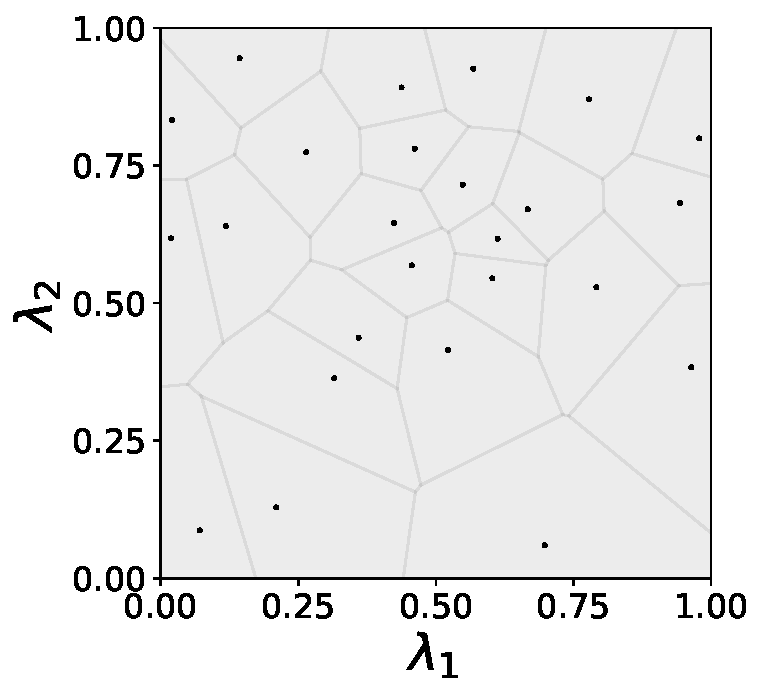
\includegraphics[width=\linewidth]{./images/voronoi_diagrams/voronoi_diagram_N25_r0}
	\end{minipage}
\caption{
Voronoi-cell discretization (partition) induced by $\nsamps = 25 $ uniform i.i.d.~random samples in $\pspace = [0,1]^2$.
}
\label{fig:voronoi_cells}
\end{figure}

The third stage then identifies the collection of Voronoi cells in $\pspace$ that approximate the contour events in $\cborel$ defined by $\qoi^{-1}(D_\idisc)$ for $\idisc=1,\hdots,\ndiscs$. This allows us to formulate the consistent solution to the discretized SIP on $(\pspace, \cborel, \contourP)$ as illustrated in step (S2) of Fig.~\ref{fig:scheme}.
The fourth stage, associated with step (S3) in Fig.~\ref{fig:scheme}, uses a discrete version of the ansatz to approximate the probability of $\VV_\iparam$ for $\iparam=1,\dots,\nsamps$.
This results in an approximate probability measure, denoted by $\updatedPxNM$, which produces the same probability estimates for events $A$ and $A\setminus \set{ \param^{(\iparam)} }_{\iparam=1}^\nsamps$, which are identical almost everywhere with respect to $\pmeas$.

Note that Algorithm~\ref{alg:inv_density} makes no mention of the method by which the samples $\set{ \param^{(\iparam)} }_{\iparam=1}^{\nsamps}$ were generated or sets in $\set{D_\idisc}_{\idisc=1}^{\ndiscs}$ are chosen.
$\set{ \param^{(\iparam)} }_{\iparam=1}^{\nsamps}$ may be generated using uniform random sampling, Latin-hypercube sampling, or even regular grids.
A thorough discussion of the choices involved in making such decisions is beyond the scope of this work, though we touch briefly on the discretization of $\dspace$ in the following section.


% Descriptions of Error
\subsection{Descriptions of Error}\label{sec:set-error}

Recall that we assumed $\dataP$ is absolutely continuous with respect to $\dmeas$, which allows us to describe $\dataP$ with a density $\rho_\dspace$. Then, for any partition $\set{D_\idisc}_{\idisc=1}^{\ndiscs}$ of $\dspace$,
\[
\dataP (D_\idisc) = \int_{D_\idisc} \observed \, \dmeas, \quad \text{ for } \idisc = 1, \hdots, \ndiscs.
\]

We often use Monte Carlo approximations to compute the approximations $p_{\dspace, \idisc}=\dataP(D_\idisc)$ in the first for-loop in Algorithm~\ref{alg:inv_density}.
These samples are generated on $\dspace$ and do not require numerical solutions to the model.
We therefore assume that for any discretization of $\dspace$, these approximations can be made sufficiently accurate and neglect the error in this computation.

We denote the exact solution to the SIP associated with this partitioning of $\dspace$ by $\PP_{\pspace, \ndiscs}$.
In situations where $\qoi(\param^{(\iparam)})$ is estimated (e.g. by application of a functional on a finite-element solution to a PDE), the approximate solutions to the SIP given in the final for-loop of Algorithm~\ref{alg:inv_density} are denoted by $\PP_{\pspace, \ndiscs, \nsamps, h}$.
Here, the $h$ is in reference to a mesh or other numerical parameter that determines the accuracy of the numerical solution $u_h(\param^{(\iparam)})\approx u(\param^{(\iparam)})$, and subsequently the accuracy in the computations of $\qoi_\iparam = \qoi(\param^{(\iparam)})$ in Algorithm~\ref{alg:inv_density}.
Then, by repeated application of the triangle inequality,
\begin{equation}
\label{eq:set-triangleineq}
d(\PP_{\pspace, \ndiscs, \nsamps, h}, \paramP) \leq
\underset{ \text{(E1)} }{\underbrace{d(\PP_{\pspace, \ndiscs, \nsamps, h},\PP_{\pspace, \ndiscs, \nsamps})}} +
\underset{ \text{(E2)} }{\underbrace{d(\PP_{\pspace, \ndiscs, \nsamps}, \PP_{\pspace, \ndiscs}) }}+
\underset{ \text{(E3)} }{\underbrace{d(\PP_{\pspace, \ndiscs}, \paramP) }}.
\end{equation}

The term (E1) describes the effect of the error in the numerically evaluated $\qoi_\iparam$ on the solution to the SIP.
The term (E2) describes the effect of finite sampling error in $\pspace$ on the solution to the SIP and (E3) describes the effect of discretization error of $\dataP$ on the solution to the SIP.

We assume that $h$ is tunable so that for any $A\in \pborel$,
\[
\lim\limits_{h \downarrow 0} \PP_{\pspace, \ndiscs, \nsamps, \imesh} (A) = \PP_{\pspace, \ndiscs, \nsamps} (A).
\]
It is possible to prove the convergence of $\PP_{\pspace, \ndiscs, \nsamps, \imesh} (A) \to \paramP (A)$ for some $A\in \pborel$ and on estimating the error in $\PP_{\pspace, \ndiscs, \nsamps, h}(A)$.
For example, in \cite{BGE+15}, adjoint-based a posteriori estimates in the computed QoI are combined with a statistical analysis to both estimate and bound the error in $\PP_{\pspace, \ndiscs, \nsamps, \imesh} (A)$.
In [TK - cite JNME 2019], adjoints are used to compute both error and derivative estimates of $\qoi(\param^{(\iparam)})$ to improve the accuracy in $\PP_{\pspace, \ndiscs, \nsamps, \imesh} (A)$.
Since the error due to $\imesh$ can be estimated as described in previous studies, and $\ndiscs$ can be made arbitrarily large, we neglect (E1) and (E3) here.
Thus, we limit our focus to (E2), where certain geometric properties of the QoI map are known to significantly impact this term, as we show below.



%%%%%

\subsection{Impact of QoI on Solution Quality }\label{sec:impact}

In the explicit (set-based) approach, a finite numerical approximation of (often uncountably many) events in $\sa$s is required.
Thus, there are two primary sources of approximation error: (1) partitioning the parameter space $\pspace$ to approximate events in $\pborel$, and (2) partitioning the data space $\dspace$ to approximate events in $\dborel$.

A non-intrusive sample-based algorithm is initially introduced in \cite{BET+14} and further analyzed in \cite{BET+14-arxiv}.
We direct the interested reader to \cite{BET+14-arxiv} for more detailed information and analysis of this algorithm, in which $\dspace$ is discretized by $M$ samples and $\pspace$ is discretized by $N$ samples.
If $\updatedP$ represents the updated probability measure, then we let $\updatedPxM$ be the exact solution to the approximate inverse problem using the discretization of $\predictedP$ by $M$ samples.
Finally, let $\updatedPxNM$ denote the approximate solution to the approximate problem under both aforementioned discretizations, so
\[
\updatedP = \lim\limits_{M\to\infty} \updatedPxM = \lim\limits_{M\to\infty} \lim\limits_{N\to\infty} \updatedPxNM.
\]

If numerical error in the evaluation of the QoI map $\qoi$ is inherent (e.g. owing to a mesh choice, surrogate model, or solution basis order), in the $N$ evaluations of samples in $\pspace$, then we let $\updatedPxNMh$ denote the approximate solution given the model discrepancy, and we have
\[
\updatedPxNM= \lim\limits_{h \downarrow 0} \updatedPxNMh.
\]

Here, the $h$ refers to a mesh or other numerical parameter that determines the accuracy of the numerical solution evaluation of the QoI map.


In \cite{BM17}, the focus is on proving the convergence of $\updatedPxNMh(A) \to \PP_{\pspace} (A)$ for some $A\in \pborel$ and on estimating the error in $\updatedPxNMh(A)$.
There, as well as in \cite{JWW17}, adjoint-based a posteriori estimates in the computed QoI are combined with a statistical analysis to both estimate and bound the error in $\updatedPxNMh (A)$.
In \cite{BM17}, adjoints are used to compute both error and derivative estimates of the QoI map to improve the accuracy in $\updatedPxNMh (A)$.
%However, no work has to date fully explored the \emph{convergence rates} of Algorithm \ref{alg:inv_density}.
%Furthermore, no work has yet to establish that these rates are independent of the choice of QoI map despite other studies establishing that the absolute error is very much affected by the geometric properties of the QoI maps \cite{BE13}.

As mentioned earlier, stability results are with respect to the Total Variation metric, which we use to study convergence as well.
Repeated application of the triangle inequality yields
\begin{equation}
\label{eq:triangleineq}
d_{\text{TV}}(\updatedPxNMh, \updatedP) \leq
\underset{ \text{(E1)} }{\underbrace{ d_{\text{TV}}(\updatedPxNMh, \updatedPxNM)}} +
\underset{ \text{(E2)} }{\underbrace{ d_{\text{TV}}(\updatedPxNM, \updatedPxM) }}+
\underset{ \text{(E3)} }{\underbrace{ d_{\text{TV}}(\updatedPxM, \updatedP) }}.
\end{equation}
The term (E1) describes the effect of the error in the numerically evaluated $Q_j$ on the solution to the stochastic inverse problem.
The term (E2) describes the effect of finite sampling error in $\pspace$, and (E3) describes the effect of discretization error of $\predictedP$ on the solution to the stochastic inverse problem.
In our experience, terms (E1) and (E3) are more easily controlled.
Thus, we limit our focus to (E2), where certain geometric properties of the QoI map are known to significantly impact this term, as we show below.


\section{Skewness and Information Content}\label{sec:skewness}
In \cite{BGE+15}, the concept of skewness in a QoI map $\qoi$ is introduced, quantified, and related to the accuracy in solving the stochastic inverse problem with a finite number of samples.
In effect, skewness is a geometric property that describes how the right angles in generalized rectangles belonging to $\dborel$ are transformed by $\qoi^{-1}$.
An a priori analysis demonstrated that the number of samples from a {\em regular uniform grid} in $\pspace$ required to approximate the $\pmeas$-measure of $\qoi^{-1}(E)$ to a desired level of accuracy is proportional to the skewness of $\qoi$ raised to the ($d-1$) power where $d$ is the dimension of $\dspace$.
This is a version of the so-called curse-of-dimension for the explicit approach.

Skewness is explored further in \cite{Walsh} in the context of optimal experimental design.
There, an additional geometric property of $\qoi$ related to the \emph{precision} in the solution of the associated stochastic inverse problem is introduced and quantified.
For completeness, we define skewness below and refer the interested reader to \cite{BGE+15, BPW17, Walsh} for more details.

\begin{defn}
For any QoI map $\qoi$, $\param \in \pspace$, and a specified row vector $\bf{j}_k$ of the Jacobian $J_{\param, Q}$, we define
\begin{equation}
S_\qoi(J_{\param,Q}, \bf{j}_k) := \frac{\abs{\bf{j}_k} }{\abs{\bf{j}_k^\perp}}.
\label{eq:skewness}
\end{equation}

We define the \textbf{local skewness} of a map $\qoi$ at a point $\pspace$ as
\begin{equation}
S_\qoi(\param) := \max_{1\leq k \leq d} S_\qoi(J_{\param,Q}, \bf{j}_k).
\label{eq:localskewness}
\end{equation}
\end{defn}

\begin{defn}
The \textbf{average} \emph{(or \textbf{expected})} \textbf{skewness} is defined as
\begin{equation}
\overline{S_Q} := \frac{1}{\mu_{\pspace}(\pspace)} \int_\pspace S_Q (\param) \, d\mu_{\pspace}
\label{eq:avgskew}
\end{equation}
\end{defn}

In \cite{BPW17}, it is shown that $S_\qoi(\param)$ is efficiently computed using a singular value decomposition of the Jacobian $J_{\param,Q}$.
In general, we approximate $\overline{S_Q}$ with Monte-Carlo approximations.

%%%%%%%%%%%%%%%%%%%%%%%%%%%%%%%%
We demonstrate the effect of skewness on the explicit measure theoretic approach in the following example.

\subsubsection{Motivating Example}

\begin{ex}
\label{ex:skewness}
Consider the following family of linear maps:
\begin{equation}\label{eq:qmap2}
\left \lbrace \qoi^{(s)} =  \mat{cc}{1 & 0 \\ \sqrt{s^2 - 1}& 1 } \right \rbrace_{s\in S},
\end{equation}
for $S=\set{1,2,4}$. These maps are designed to control the global skewness (since it is equal to local skewness in a linear map), while preserving the measures of sets between $\pspace$ and $\dspace$.
More specifically, the support of $\updatedP$ associated with each QoI map using uniform observed measures have equal $\pmeas$-measure, which isolates the impact of accuracy solely to the skewness of the QoI map.

The skewness of these maps is given by the index $s$, so $\qoi^{(1)}$ is $1$, the skewness of $\qoi^{(2)}$ is $2$, and $S_{\qoi^{(4)}} = 4$.



\begin{figure}[ht]
\begin{minipage}{.65\textwidth}
\begin{table}[H]
\begin{tabular}{ c | c | c | c }
N & $\qoi^{(a)}$ & $\qoi^{(b)}$ & $\qoi^{(c)}$\\ \hline \hline
$200$ & $2.97E-01$ & $3.42E-01$ & $5.28E-01$\\ \hline

$400$ & $2.00E-01$ & $2.41E-01$ & $3.79E-01$\\ \hline

$800$ & $1.59E-01$ & $1.78E-01$ & $2.88E-01$\\ \hline

$1600$ & $1.06E-01$ & $1.31E-01$ & $1.93E-01$\\ \hline

$3200$ & $8.38E-02$ & $9.39E-02$ & $1.41E-01$\\ \hline

$6400$ & $6.14E-02$ & $6.40E-02$ & $1.05E-01$\\ \hline

\end{tabular}
\end{table}

\end{minipage}
\begin{minipage}{.65\textwidth}
		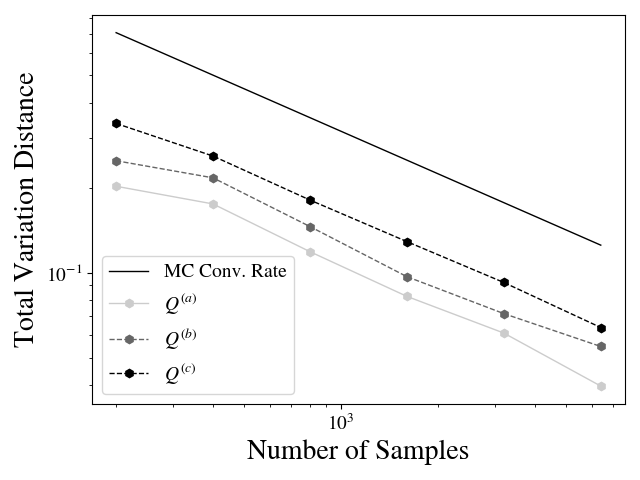
\includegraphics[width=\linewidth]{./images/Plot-reg_BigN_40000_reg_M_1_rand_I_100000}
\end{minipage}
\caption{The results of $d_\text{TV}(\updatedPxNM, \updatedPxNN)$.}
\label{fig:skew}
\end{figure}

It is evident in Figure~\ref{fig:skew} that skewness has a direct impact on the number of samples required to achieve a given accuracy.
We see that the measure induced by $\qoi^{(1)}$ requires fewer than half the number of samples to be as accurately resolved as $\qoi^{(2)}$ does.
The effect is even more pronounced when compared against $\qoi^{(4)}$.

This provided a strong motivation for minimizing skewness and reinforces the results from \cite{BPW_2015}, where it is demonstrated that a similar relationship existed in the number of samples required to remove error in inverse set approximations quantified by the $\pmeas$-measure of the {\em symmetric difference} of the inverse sets.

\end{ex}

The example above motivates a number of research directions involving how to resolve approximation errors.
How the Data Consistent Inversion framework handles the skewness in QoI maps is unclear and requires numerical studies to investigate, which we perform herein [TK - cite where].

%%%%%%%%%%%%%%%%%%%%%%%%%%%%%%%%%%%%
%%%% discussion of convergence

\subsection{Convergence}
Second, and perhaps most importantly, since the spaces $\pspace$ we are considering are generally bounded and finite, the Total Variation metric metrizes weak convergence (see Thm. 6 in \cite{GS02}).
The latter property is of notable importance because the QoI maps we study are indeed (component-wise) functionals on the space of model inputs $\pspace$.
Thus, convergence of a sequence of probability measures under the Total Variation metric implies that the QoI's will also converge component-wise in $\RR$.
In other words, convergence in the Total Variation metric implies the convergence of the sampled QoI map to the exact QoI map since the map is a linear functional of the probability measure.
In other words, if $\PP_{\pspace,\ndiscs,\nsamps,h}$ converges to either $\PP_{\pspace,\ndiscs,\nsamps}$, $\PP_{\pspace,\ndiscs}$, or $P_\pspace$ using the Total Variation metric, this implies that the error converged to zero in the numerically computed $\qoi(\param^{(j)})$.
Thus, convergence in the Total Variation metric implies, in a sense, convergence of the numerical method used to construct the QoI map.
Furthermore, recall that weak convergence $\PP_n \to \PP$ is defined to mean
\[
\int f \PP_n \to \int f \PP \text{ as } n \to \infty
\]
for bounded Lipschitz functions $f:\pspace\to\RR$.
Taking $f = \Chi_A$, this leads to the following implication:
\[
\PP_{\pspace, \ndiscs, \nsamps} \to P_\pspace \implies \PP_{\pspace, \ndiscs, \nsamps} (A) \to P_\pspace (A) \quad \forall{A\in\pborel}.
\]
%provided we rigorously define $\P\PP_{\pspace, \ndiscs, \nsamps}$ to measure sets in $\BB_\pspace$, which we proceed to do in the following section\footnote{\bf{I know this is clumsy, but I'm not exactly sure how to phrase this correctly, because it almost seems like this would be true for all $A\in\pspace$ instead. I suppose the omission of the differential operator above is intentionally vague to gloss over this detail. Can we sharpen this up?}}
It is a combination of computational ease of implementation and theoretical implications that motivates the choice of the Total Variation as the metric used in the numerical results of Section \ref{sec:ch03-set} and \ref{sec:ch03-sample}.



\section{Accuracy of Set-Based Inversion}\label{sec:ch03-set}

%%%%%%%%%%%%%% discretization discussion, software contribution in later section



The measures computed from Algorithm~\ref{alg:inv_density} are defined on a set of samples $S = \set{\param^{(j)}}_{j=1}^{\nsamps}$ which implicitly define a Voronoi-cell partition $\set{\VV^{(j)}}_{j=1}^{\nsamps}$ of the parameter space $\pspace$.
We let $\BB_{\pspace, \nsamps}$ denote the \emph{computational algebra} generated by $\set{\VV^{(j)}}_{j=1}^{\nsamps}$, i.e., using standard measure theory notation,
$$
	\BB_{\pspace,\nsamps} = \sigma\left(\set{\VV^{(j)}}_{j=1}^{\nsamps}\right).
$$
Clearly, $\BB_{\pspace, \nsamps}\subset \BB_\pspace$ and the events $A\in B_{\pspace, \nsamps}$ represent the $A\in\BB_\pspace$ for which we can ``easily'' compute probabilities and make inferences.
While Algorithm~\ref{alg:inv_density} ultimately defines a probability measure implicitly on $(\pspace,\BB_\pspace)$, computationally this is almost never done and the measures are only interrogated on the computational algebra associated with the set of samples.

Different sets $S_k = \set{\param{(i)}}_{i=1}^{\nsamps_k}$, where the $\param^{(i)}$'s and $\nsamps_k$'s may be completely different for each $k$, will lead to different measures computed from Algorithm~\ref{alg:inv_density}.
Each $S_k$ induces a computational algebra which we index using the notation $\BB_{k}$ for simplicity, where it is understood that $\BB_k = \BB_{\pspace, \nsamps_k}$.

This poses an immediate problem with respect to a computational approach to computing $d_H$: how do we compare measures $\PP_{\pspace, \ndiscs, \nsamps_1}$ and $\PP_{\pspace, \ndiscs, \nsamps_2}$ which may be defined on completely different computational algebras (even if $\nsamps_1=\nsamps_2$)?
See Figure~\ref{fig:voronoi_issues} for an illustration of such a scenario.

\begin{figure}[ht]
\centering
	\begin{minipage}{.4875\textwidth}
		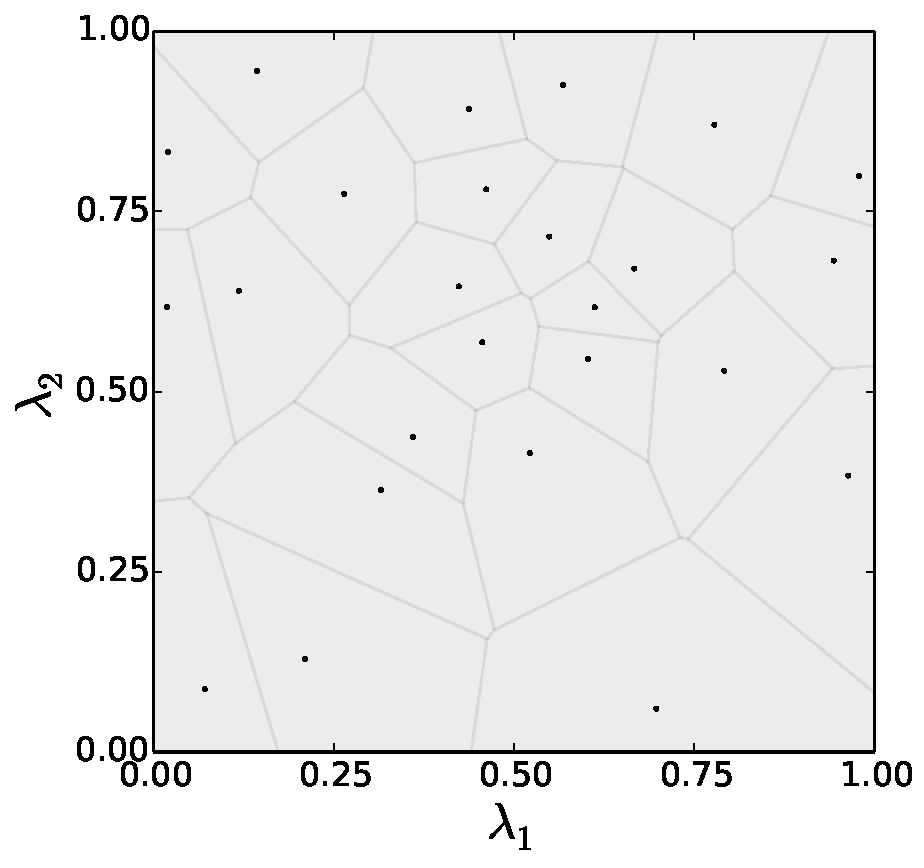
\includegraphics[width=\linewidth]{./images/voronoi_diagram_N25_r0}
	\end{minipage}
	\begin{minipage}{.4875\textwidth}
		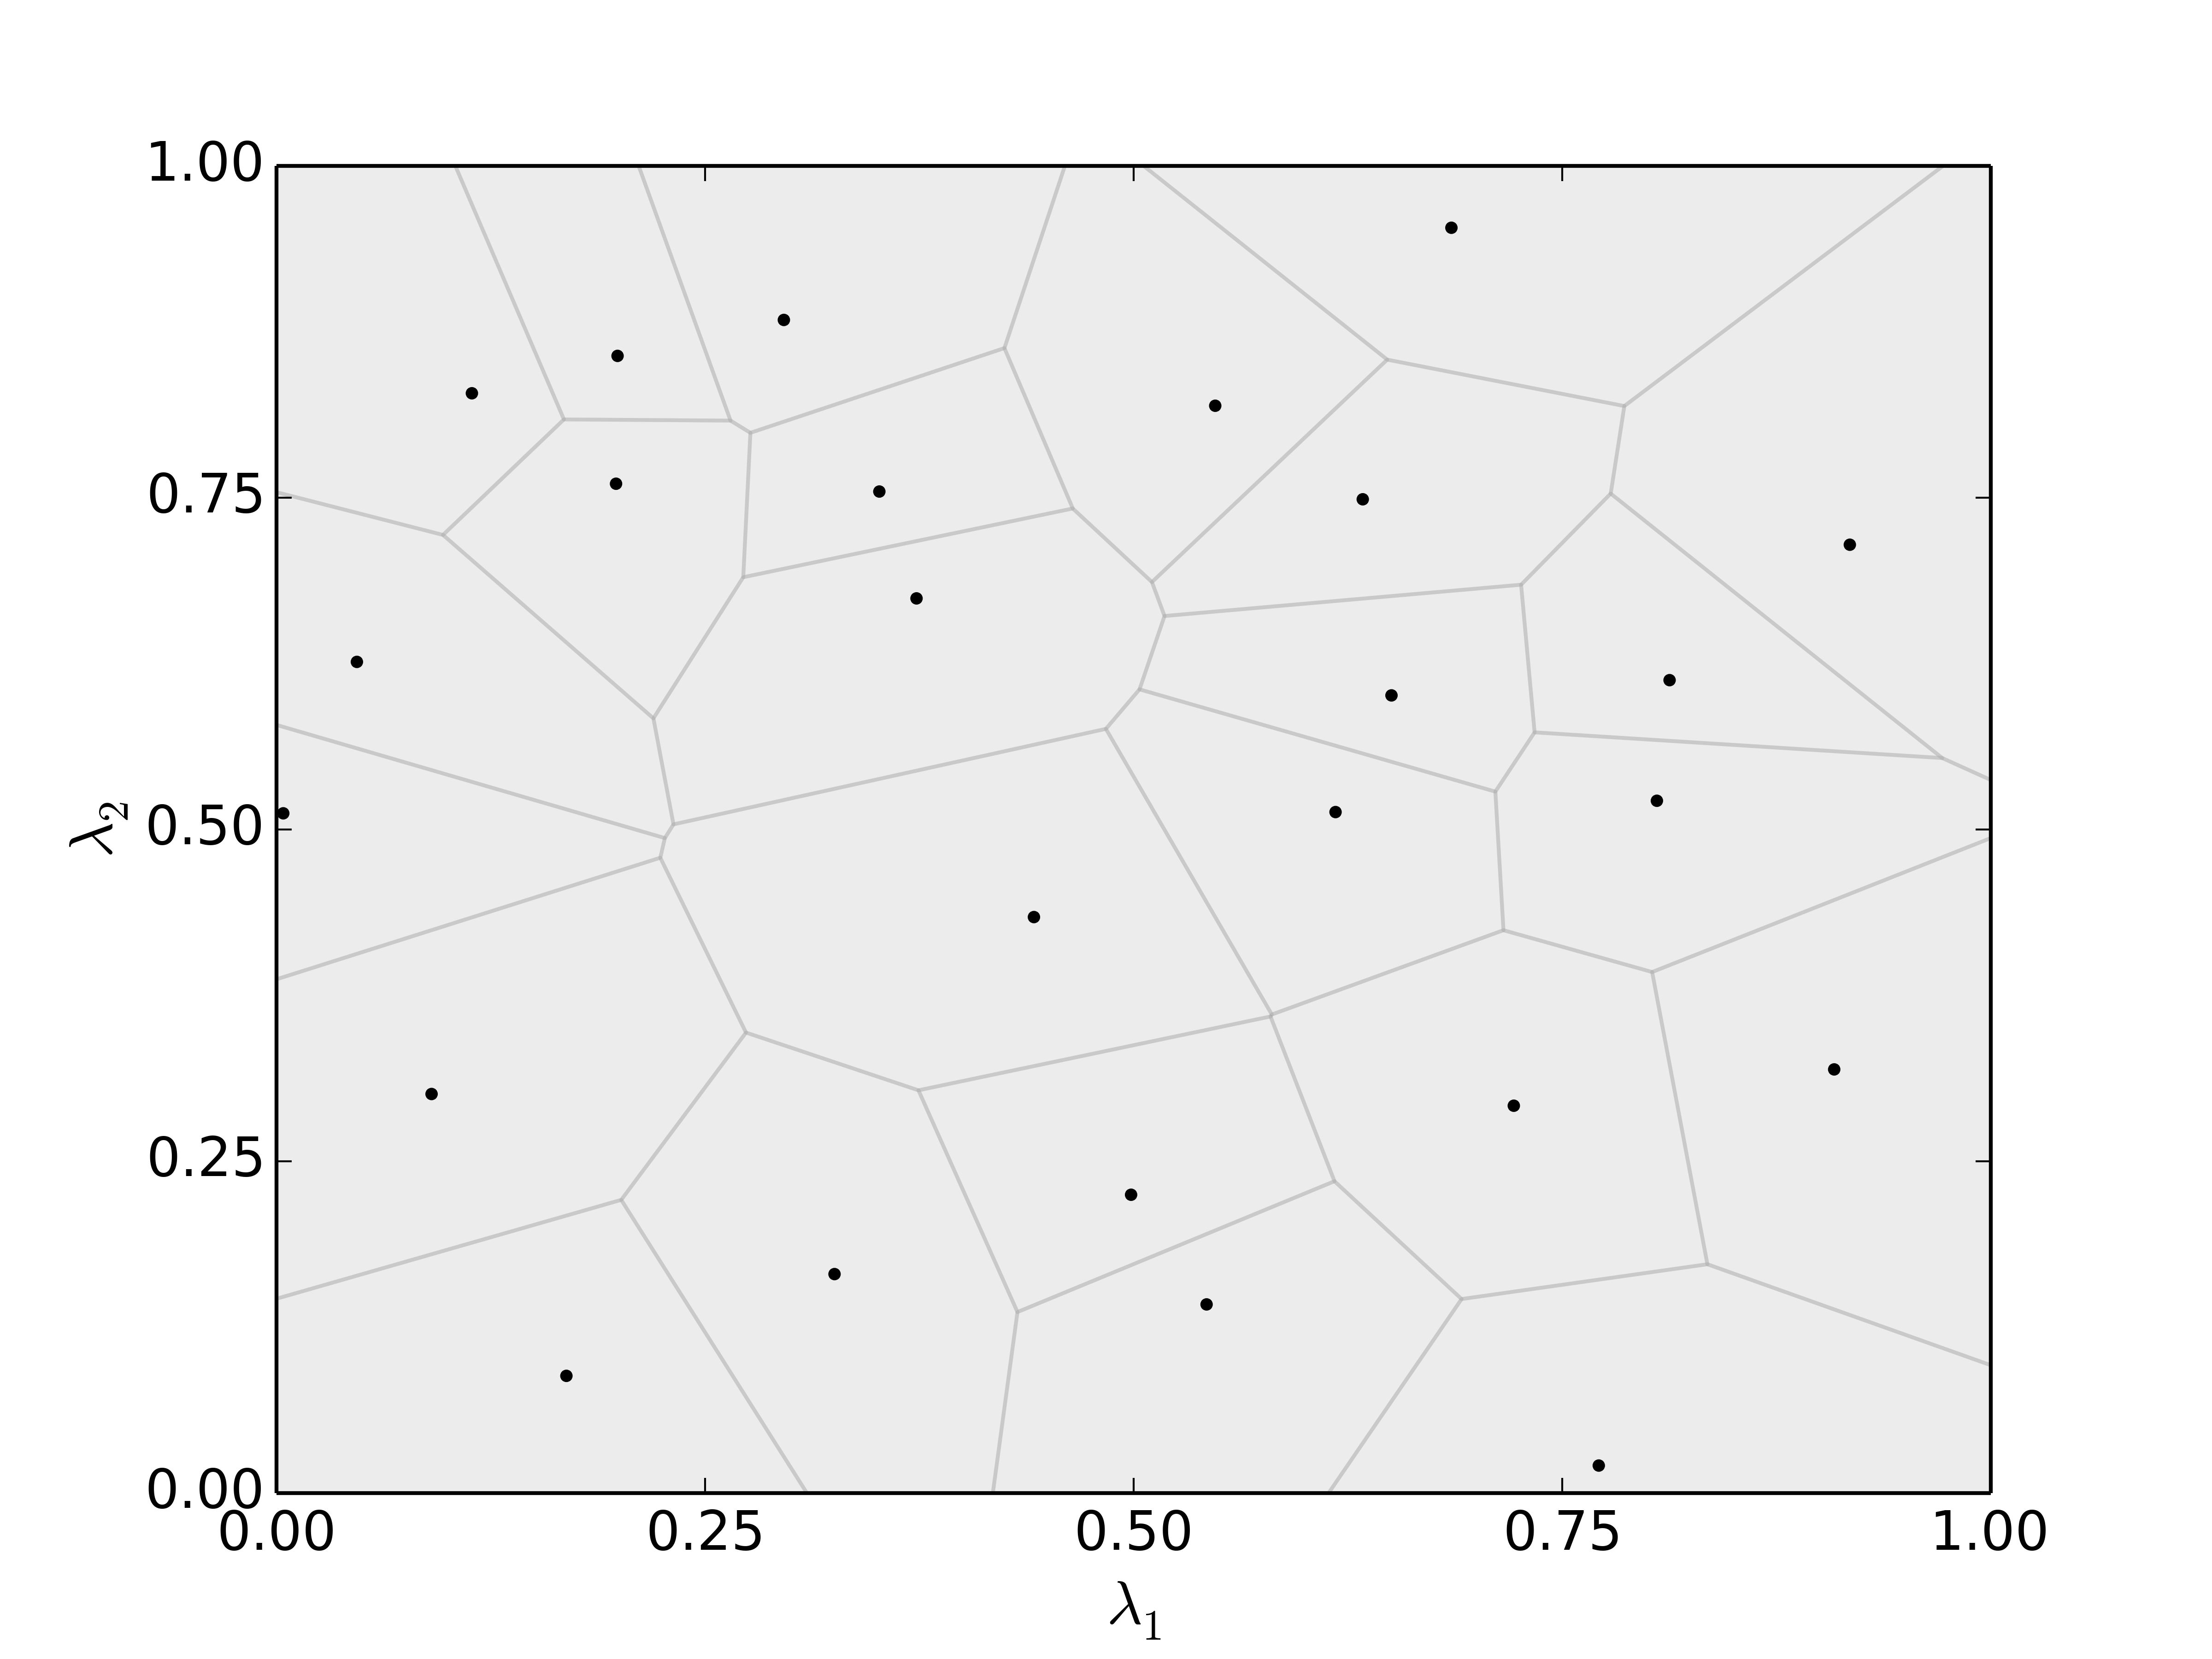
\includegraphics[width=\linewidth]{./images/voronoi_diagram_N25_r10}
	\end{minipage}
\caption{
Two different Voronoi partitions induced by $\nsamps_1 = \nsamps_2 = 25 $ uniform i.i.d.~random samples.
}
\label{fig:voronoi_issues}
\end{figure}


The proof of the following Lemma describes how to ``computationally extend'' {\em any} probability measure defined on a computational algebra to a full $\sa$ $\BB$, which we exploit in Algorithm~\ref{alg:hellinger_disc}.
\begin{lem}
\label{lem:measuresets}
Let $\mu$ be a measure on $(\pspace, \BB_\pspace)$, $\set{\VV^{(j)}}_{j=1}^{\nsamps}$ be a partition of $\pspace$, and $\BB_{\pspace, \nsamps}$ the computational algebra generated by $\set{\VV^{(j)}}_{j=1}^{\nsamps}$.
Assume $\mu (\VV^{(j)}) > 0 \; \forall \; j=1,\hdots, \nsamps$.
Then, there exists a probability measure $\eta$ on $(\pspace, \BB_\pspace)$ such that $\eta(A) = \eta_\nsamps(A) \; \forall \; A\in\BB_{\pspace, \nsamps}$.
\end{lem}
In the proof below, we use $\eta_\nsamps$ and $\mu$ to construct a type of ``discrete'' Radon-Nikodym derivative of $\eta$.
This is motivated by the formal structure of solutions given by Algorithm~\ref{alg:inv_density}.
The proof of Lemma~\ref{lem:measuresets} can be found in Appendix~\ref{app:measuresets}, but the two key equations involved are reproduced here for later reference:

\begin{equation}\label{eq:finiteradon}
f_\nsamps (\param) = \sum_{j=1}^{\nsamps} \frac{\eta_\nsamps (\VV^{(j)}) }{\mu (\VV^{(j)})} \Chi_{\VV^{(j)}} (\param).
\end{equation}

Then, for any $A\in\BB_\pspace$, define

\begin{equation}\label{eq:approxmeasure}
\eta (A) = \int_A f_\nsamps (\param) \, d\mu.
\end{equation}

We note that in practice, $\Chi_{\VV^{(j)}} (\param)$ requires the use of nearest-neighbor computations, but otherwise evaluation of Eq.~\eqref{eq:finiteradon} is straightforward to compute.
With that established, we now present the algorithm used for approximating the distances between pairs of measures (with the computational implementation discussed in \ref{sec:ch03-software}.


\begin{algorithm}
\DontPrintSemicolon
\caption{Total Variation Discretization}
\label{alg:totvar_disc}
Let $(\pspace, B_{\pspace, \nsamps_1}, \eta_{\nsamps_1} )$ and $(\pspace, B_{\pspace, \nsamps_2}, \eta_{\nsamps_2} )$ be given.\\

Construct $f_{\nsamps_1}$ and $f_{\nsamps_2}$ and corresponding $\eta_1, \eta_2$ using Eq.~\eqref{eq:finiteradon} and Eq.~\eqref{eq:approxmeasure}, respectively.

Use Monte Carlo sampling to approximate
$$ d_{TV}(\eta_1, \eta_2) = \int_\pspace f_{\nsamps_1}\lam - f_{\nsamps_2}\lam \, d\mu $$.
\end{algorithm}

Since we now have a way to extend probability measures defined on $(\pspace, \BB_{\pspace, \nsamps})$ to  probability measure on $(\pspace, \BB_{\pspace})$, we can use simple Monte-Carlo approximation schemes to the Hellinger distance between two probability measures defined on two separate computational algebras.
This is demonstrated in Algorithm~\ref{alg:hellinger_disc}.


%%%%%%%%%%%%%%%%%%%%%%%%%%%%%%%%%%%%%%%%%%%%%%%%%%%%%%%%%%%%%%
\subsection{Overview of Examples}
We establish some fundamental properties of solutions to the SIP under different QoI maps in terms of the skewness of the $Q$'s being compared.
We seek an estimated probability measure $\hat{\PP}_\pspace$ on the parameter space to converge (with respect to the metric $d_\text{TV}$) to some reference measure $\PP_\pspace$ as more samples (i.e., model evaluations), $\nsamps$ are used.
Such a reference measure could be either some known distribution taken as truth, or another approximation deemed to be sufficiently resolved for the given application or computational budget (i.e. higher-fidelity model, mesh, or Monte Carlo sample-size).\footnote{However, we could also choose to interrogate the push-forward measures given by propagating the $\hat{\PP}_\pspace$ and $\PP_\pspace$ forward to a data space by a QoI map and taking the distance on the resulting output space.
This would measure the ability of the maps to reconstruct the output probability measure.}

In Figure~\ref{fig:voronoi_sols}, we illustrate the solution to the problem of comparing measures defined on two different (implicitly-defined) $\sa$s shown in Figure~\ref{fig:voronoi_issues}.
By introducing a third set against which both sample sets of size $\nsamps=50$ are compared, we can leverage theoretical results from Lemma~\ref{lem:measuresets} to compare solutions to the SIP under different QoI maps.

\begin{figure}[ht]
\centering
	\begin{minipage}{.275\textwidth}
		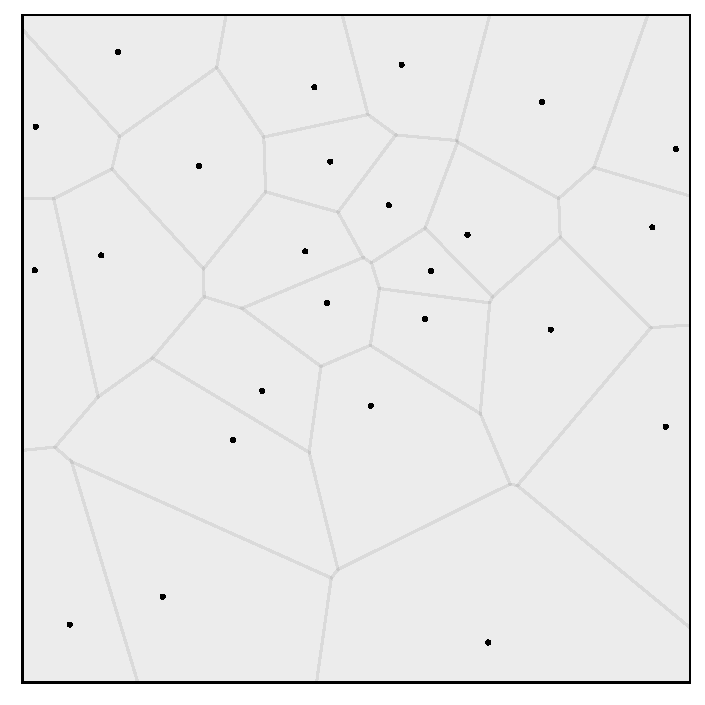
\includegraphics[width=\linewidth]{./images/voronoi_diagrams/voronoi_diagram_N25_r0_no_label}
	\end{minipage}
	\begin{minipage}{.4\textwidth}
		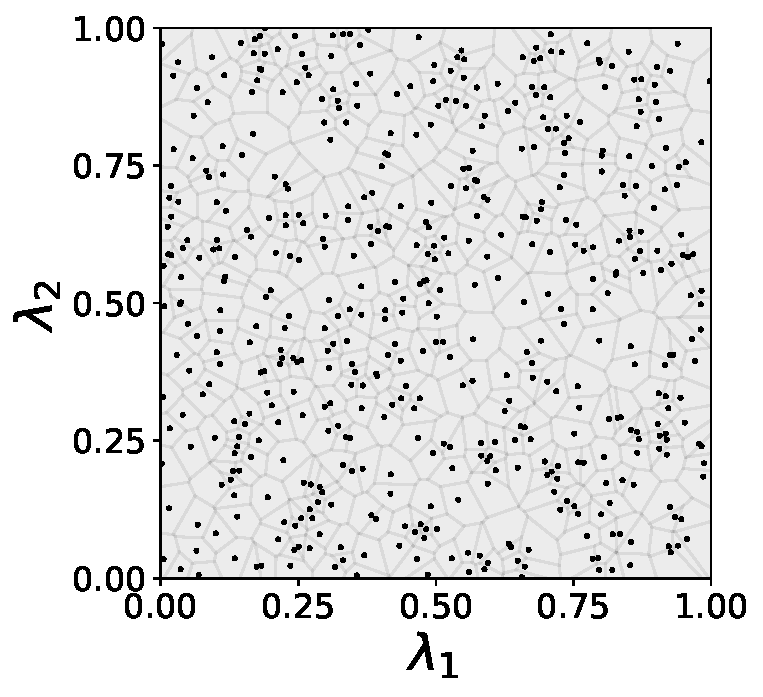
\includegraphics[width=\linewidth]{./images/voronoi_diagrams/voronoi_diagram_N500_r50}
	\end{minipage}
		\begin{minipage}{.275\textwidth}
		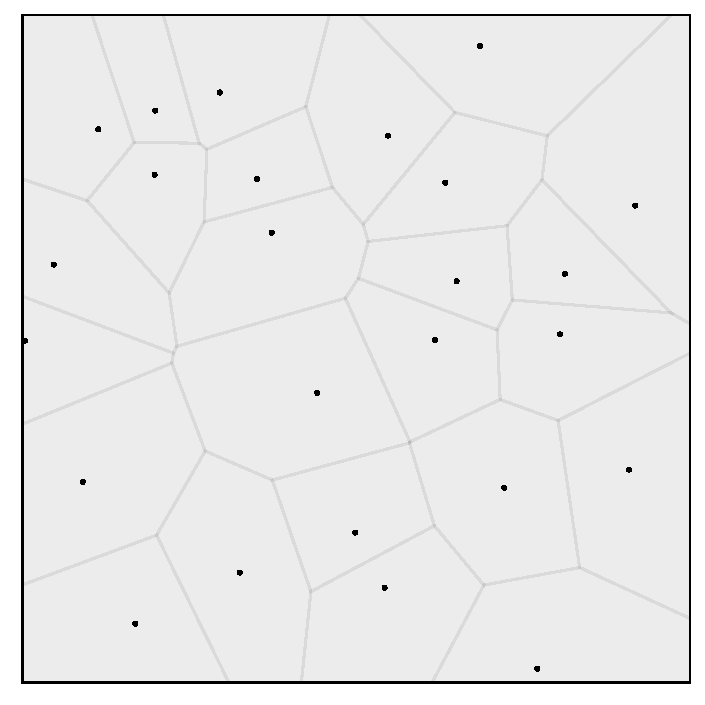
\includegraphics[width=\linewidth]{./images/voronoi_diagrams/voronoi_diagram_N25_r10_no_label}
	\end{minipage}
\caption{
(Left/Right): The two partitions from Figure~\ref{fig:voronoi_issues} will be projected onto a third reference partition (center), in order to compare them on a common $\sa$.
Center: A possibly over-resolved reference sample set, generated using $\nsamps = 500$ uniform i.i.d.~random samples.
}
\label{fig:voronoi_sols}
\end{figure}

To isolate the effect of skewness on the ability to approximate sets with finite sampling, we choose the maps so that they preserve the sizes of sets between $\pspace$ and $\dspace$ under the push-forward measure given in Eq.~\eqref{eq:dataspace_pushforward_measure}.
The sizes of these inverse sets correspond to the average precision of maps $Q$, so we fix the maps to all be equally informative from this perspective; for linear maps, this means they all have the same determinant.

All of our experiments follow the same structure, where $\qspace$ denotes a set of QoI maps under consideration in each example:
\begin{itemize}
\item[[0-a]] Select $\qoi\in\qspace$ and define $\PP_{\dspace_\qoi}$ as a uniform distribution centered on a reference QoI value $Q(\paramref)$ for $\paramref$ taken as the midpoint of $\pspace$.
Note that $\PP_{\dspace_\qoi}$ is exactly discretized with $M=1$ sample, so that
\[
P_{\pspace, 1} = P_\pspace.
\]
\item[[0-b]] Create a regular grid of samples in $\pspace=[0,1]^n$ using $N_{\text{ref},i}$ equispaced points in each dimension.
Set $\bar{N} := \prod N_{\text{ref},i}$.
Since $n$ is small in the numerical examples shown here, we select $N_{\text{ref},i} = 200 \; \forall \; i$ in each example.
\item[[0-c]] Use Algorithm~\ref{alg:inv_density} to construct a reference solution $\PP_{\pspace,\bar{N}}\approx \PP_\pspace$.
\item[[1]] Generate $\set{S_k^{(n)}}_{n=1}^{50}$ sets of uniform i.i.d.~random samples where $N_k = 25, 50, 100, 200, \hdots, 6400$, and $n$ represents the number of repeated trials of a sample size $N_k$.
%, constructing $\set{\set{\VVV_k^{(j)}}_{k=1}^{50}}_{j=1}^{N}$ so that when we compute Total Variation distances on the approximate measures defined on each $\set{\VVV_k^{(j)}}{j=1}{N}$, we can reduce the variance in our expected Total Variation distance values for each instance of $N$. Note that we experimented with using more trials and found the variance in expected Total Variation distances was sufficiently low with as few as twenty trials for the maps under consideration herein.
%\item[[3]] For every trial $T$ and $N$ value (including $\bar{N}$), the reference parameter $\lambda = (\lambda_1, \lambda_2) = (0.5, 0.5)$ is mapped by $Q$ to $\dspace_\qoi = Q(\pspace)$.
%\item[3] A uniform distribution with support $[Q(\lambda_1) - 0.05, Q(\lambda_1) + 0.05] \times [Q(\lambda_2) - 0.05, Q(\lambda_2) + 0.05]$ is defined on $\dspace_\qoi$, representing equal uncertainty in each component of our measured functional values.
\item[[2]] Solve the SIPs using Algorithm~\ref{alg:inv_density} to construct $\set{\PP_{\pspace,M,N}^{(n)}}_{n=1}^{50}$.
\item[[3]] Use $1E5$ i.i.d.~random samples to estimate $\set{d_H^2( \PP_{\pspace,M,N}^{(n)}, \PP_{\pspace,\bar{N}})}_{n=1}^{50}$.
\item[[4]] Average over all trials $n$ for each $N$ to estimate the {\em expected} Total Variation distance for $N$ samples and analyze convergence to $\PP_{\pspace,\bar{N}}$.
\item[[5]] Repeat steps [0-a]--[4] for each $\qoi\in\qspace$ under consideration.
\end{itemize}

\FloatBarrier

\subsection{Rotational Invariance}\label{ex:rotation}
This example shows that if $\qoiA$ is defined by a rotation of $\qoiB$, then the accuracy and convergence rates of $\PP^{(a)}_{\pspace, \ndiscs, \nsamps}$ are identical to $\PP^{(b)}_{\pspace, \ndiscs, \nsamps}$.
We expect this to be true since skewness is rotationally invariant, as we summarize in the following Proposition.
\begin{prop}
The quantity $S_\qoi(\param)$ is invariant under rotations performed on $\qoi$ for any $\param$. \\
\label{prop:rot_invariance}
\end{prop}
\begin{proof}
If we apply a rotation $\qoi$, then the Jacobians $J_{\qoi, \param}$ are also subject to the same rotation at each $\param$.
Since rotations are unitary operators, the norms given in Eq.~\eqref{eq:skewness} used to define skewness are unaffected.
\end{proof}

\begin{figure}
\begin{minipage}{.5\textwidth}
\begin{table}[H]
\begin{tabular}{ c | c | c | c }
\nsamps & $\qoiA$ & $\qoiB$ & $\qoiC$\\ \hline \hline
$200$ & $2.18E-01$ & $1.97E-01$ & $2.19E-01$\\ \hline

$400$ & $1.60E-01$ & $1.70E-01$ & $1.51E-01$\\ \hline

$800$ & $1.09E-01$ & $1.14E-01$ & $1.09E-01$\\ \hline

$1600$ & $7.43E-02$ & $7.76E-02$ & $7.53E-02$\\ \hline

$3200$ & $5.51E-02$ & $5.53E-02$ & $5.31E-02$\\ \hline

$6400$ & $4.19E-02$ & $4.09E-02$ & $4.19E-02$\\ \hline
\end{tabular}
\end{table}
\end{minipage}
\begin{minipage}{.45\textwidth}
		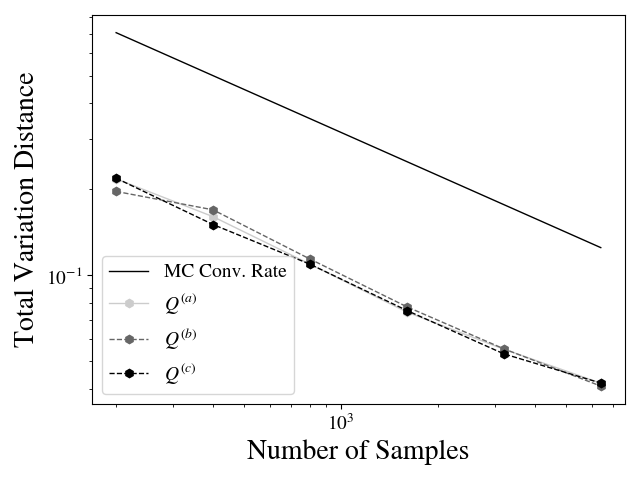
\includegraphics[width=\linewidth]{./images/Plot-orth-reg_BigN_40000_reg_M_1_rand_I_100000.png}
\end{minipage}
\caption{The results of $d^2_\text{TV}(\PP_{\pspace, \ndiscs, \nsamps}, \PP_{\pspace, \bar{\nsamps}})$ for three maps generated by random rotations of orthogonal linear maps.}
\label{fig:M1orth}
\end{figure}

To demonstrate this Lemma numerically, we define the space of QoI maps $\qspace = \set{ \qoiA , \qoiB, \qoiC }$, where all three are linear maps with the same local skewness $S_\qoi (\param) = 1 \; \forall \param \in \pspace$.
The map $\qoiA$ is the identity and the other two, $\qoiB$ and $\qoiC$ are rotations of $\qoiA$ by randomly chosen angles.
Following the algorithmic outline above, we perform a convergence study to $\PP_{\pspace,\bar{\nsamps}}$ with results summarized in Figure~\ref{fig:M1orth}.
The convergence rates and expected errors in the SIPs associated with each of these maps are virtually indistinguishable.
In light of Proposition~\ref{prop:rot_invariance} and these numerical results, we conclude that the accuracy of the numerical solution to the SIP is invariant under rotations to the QoI map.

\FloatBarrier

%%%% 2D Skewness Example %%%%%% 
\subsection{Impact of Skewness on Accuracy}\label{ex:skewness}
In this example, we demonstrate the key point of this study: the magnitude of skewness between QoI impacts accuracy by orders of magnitude, and thus in optimizing the choice of a QoI map, it is in our interest to pursue the minimization of skewness. 
This is especially true in problems where the number of random samples we are permitted to use is constrained by the computational cost of model evaluations.

%Thus, any map can be thought of as a piecewise-defined linear map, and the results we present in this example, while applying to all of $\pspace$ in these cases, can be applied solely to the support of each local linear approximation.
%Capturing the geometry of sets (improving accuracy) on each of these subdomains thus guarantees a desired result on the entirety of the domain. 

To illustrate this point, we first define the linear maps 
\begin{equation}\label{eq:qmap2}
\qspace_S := \left \lbrace Q^{(s)} =  \mat{cc}{1 & 0 \\ \sqrt{s^2 - 1}& 1 } \right \rbrace_{s\in S},
\end{equation}
for $S=\set{1,2,4}$ because they allow us to control the global skewness (since it is equal to local skewness in a linear map) while preserving the measures of sets between $\pspace$ and $\dspace$. 
More specifically, the support of the solution to the SIP associated with each QoI map has equal $\mu_\pspace$-measure, which isolates the impact of accuracy solely to the skewness of the QoI map.
We show what the component row vectors of these maps in Figure~\ref{fig: skewmapvecs} and note the skewness is determined by the ratio of the magnitude of the black line to its projection onto the vertical axis (and each of these projects directly on to the unit vector).  
The skewness of these maps is given by the index $s$, so $Q^{(1)}$ is $1$, the skewness of $Q^{(2)}$ is $2$, and $S_{Q^{(4)}} = 4$.

The maps chosen for this example are expository ones that provide valuable insight despite their simplicity. 
For example, when solving many physics-based problems, local linear approximations are often used to simplify model evaluation and guide optimization procedures.


\begin{figure}[h]
	\begin{minipage}{.3\textwidth}
		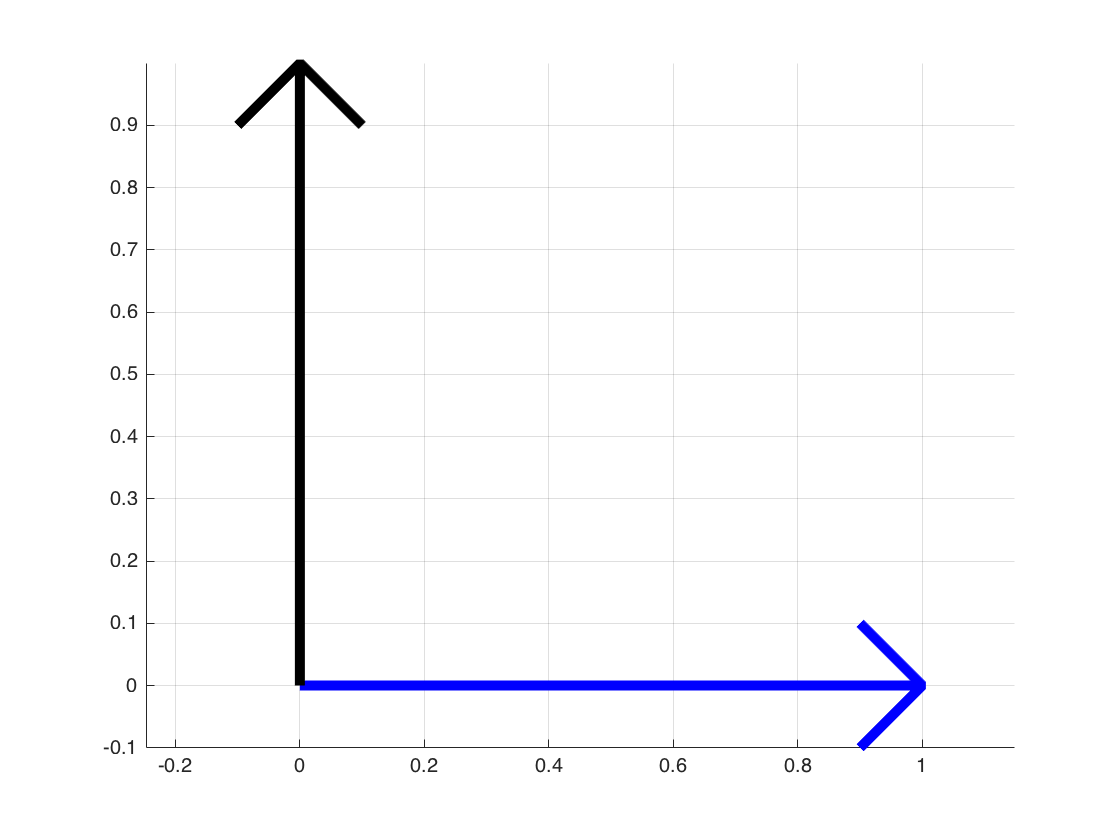
\includegraphics[width=\linewidth]{./images/vector_a.png}
	\end{minipage}
	\begin{minipage}{.3\textwidth}
		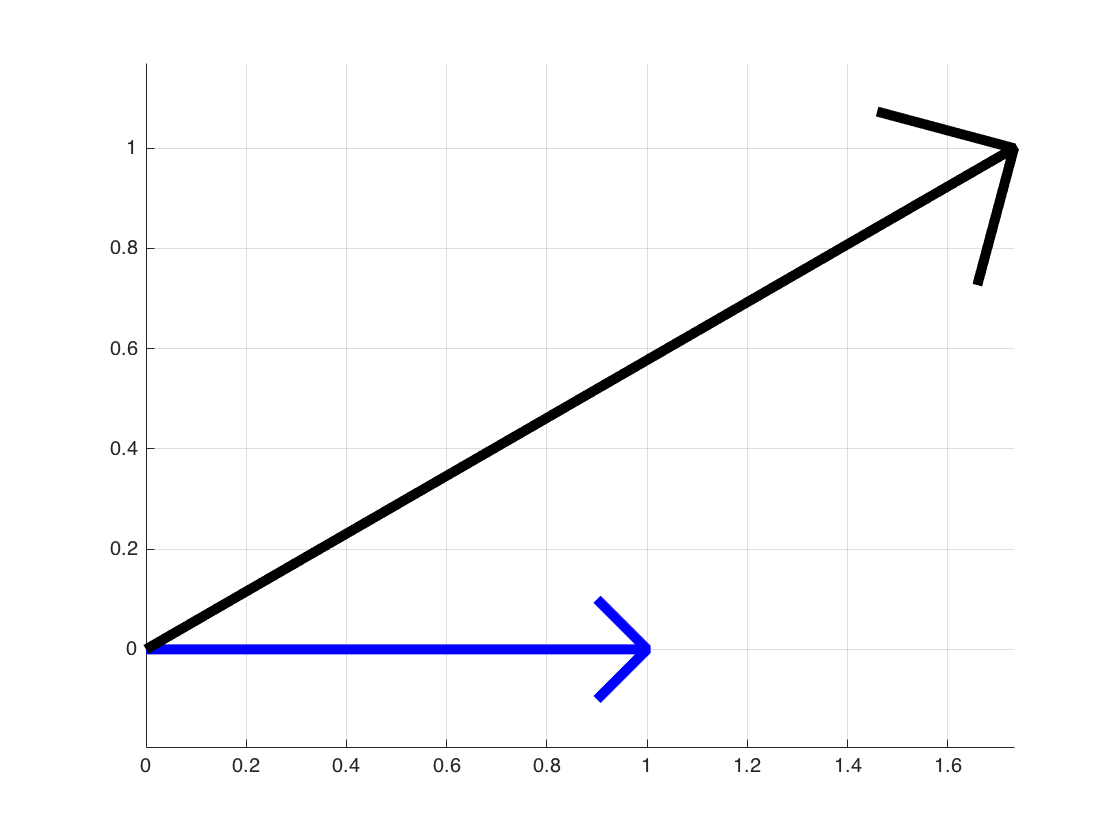
\includegraphics[width=\linewidth]{./images/vector_b.png}
	\end{minipage}
	\begin{minipage}{.3\textwidth}
		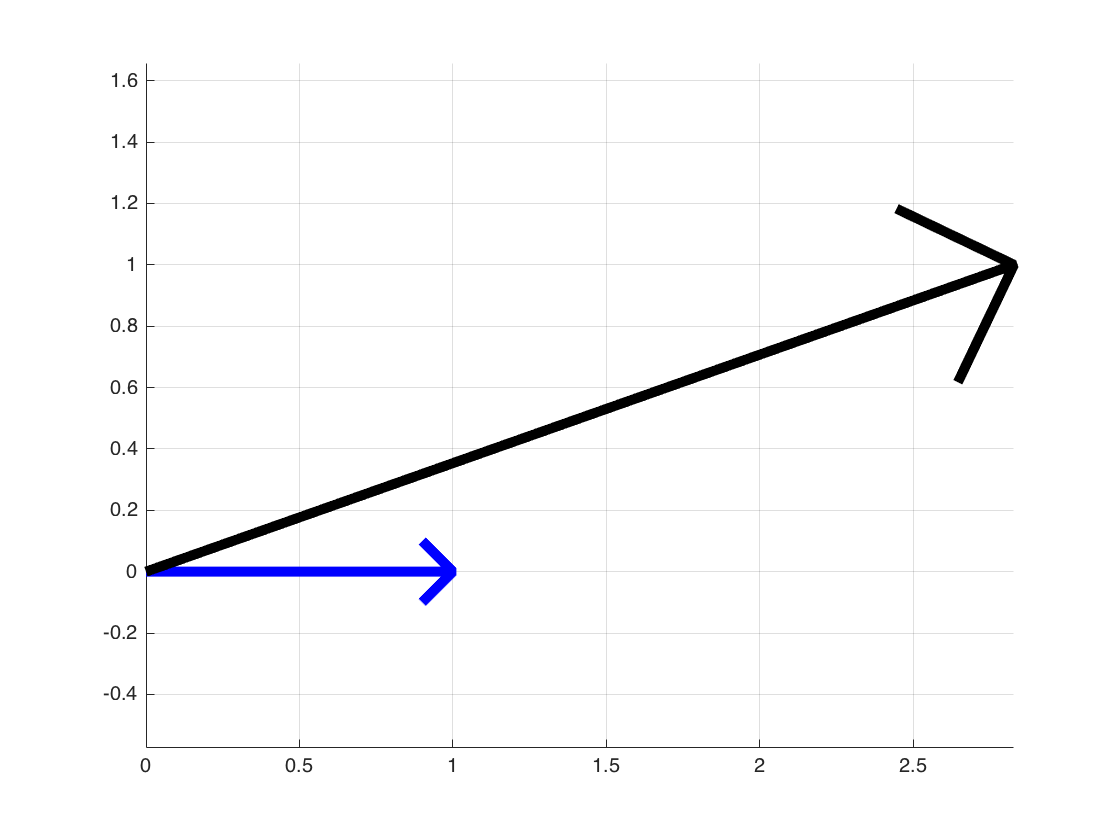
\includegraphics[width=\linewidth]{./images/vector_c.png}
	\end{minipage}
\caption{(Left to right):  The component row-vectors of $Q^{(1)}$, $Q^{(2)}$, and $Q^{(4)}$. Our linear maps take $\RR^2$ to $\RR^2$ and can be visualized graphically as the component row-vectors of the matrices representing the transformation. The first row is highlighted in blue. The skewness is then simply equal to the reciprocal of the inverse sine of the angle between these vectors. }
\label{fig: skewmapvecs}
\end{figure}


\begin{figure}
\begin{minipage}{.5\textwidth}
\begin{table}[H]
\begin{tabular}{ c | c | c | c }
N & $Q^{(1)}$ & $Q^{(2)}$ & $Q^{(4)}$\\ \hline \hline
$200$ & $1.35E-01$ & $2.03E-01$ & $3.12E-01$\\ \hline 
 
$400$ & $9.96E-02$ & $1.47E-01$ & $2.15E-01$\\ \hline 
 
$800$ & $7.19E-02$ & $1.04E-01$ & $1.53E-01$\\ \hline 
 
$1600$ & $5.27E-02$ & $7.49E-02$ & $1.10E-01$\\ \hline 
 
$3200$ & $3.70E-02$ & $5.25E-02$ & $7.52E-02$\\ \hline 
 
$6400$ & $2.76E-02$ & $3.86E-02$ & $5.54E-02$\\ \hline 
\end{tabular}
\end{table}
\end{minipage}
\begin{minipage}{.45\textwidth}
		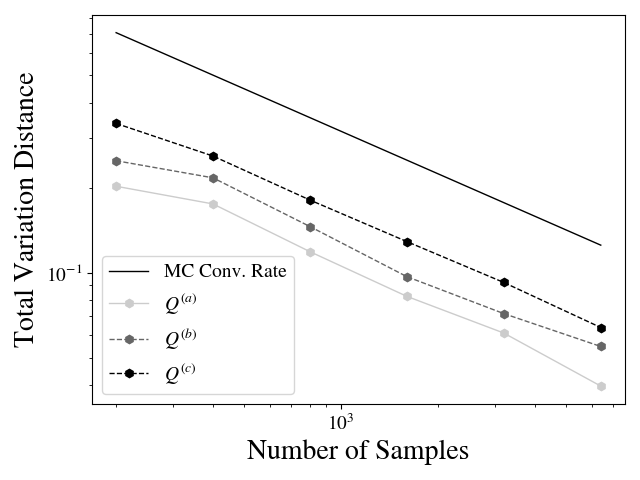
\includegraphics[width=\linewidth]{./images/Plot-reg_BigN_40000_reg_M_1_rand_I_100000}
\end{minipage}
\caption{The results of $d^2_H(\PP_{\pspace, M, N}, \PP_{\pspace,\bar{N}})$.}
\label{fig:M1_2d}
\end{figure}

We see in Figure~\ref{fig:M1_2d} that skewness has a very direct impact on the number of samples required to achieve a particular value for the Hellinger distance. 
We can see that the measure induced by $Q^{(1)}$ requires fewer than half the number of samples to be as accurately resolved as $Q^{(2)}$ does. 
The effect is even more pronounced when compared against $Q^{(4)}$.
It appears that if the ratio of skewness between two maps is 2, then the more-skewed map will require at least twice as many random samples to approximate the set on a a well-resolved discretization with the same error tolerance.

This provides a strong motivation for minimizing skewness and reinforces the results from \cite{BPW_2015}, where it was demonstrated that a similar relationship existed in the number of samples required to remove error in inverse set approximations quantified by the $\mu_\pspace$-measure of the {\em symmetric difference} of the inverse sets.




%%%% 3D Skewness Example %%%%%%

\subsection{Dependence on Dimension}\label{ex:3dmap}
To further illustrate that relationship between skewness and accuracy holds as we move towards higher dimensions, we extend the numerical investigation to a three--dimensional parameter space.
Generally, we have fewer QoI than number of uncertain model parameters, so we assume that the potential QoI maps are defined by the $2\times 3$ matrices
\begin{equation}\label{eq:qmap3}
\qspace_S := \left \lbrace \qoi^{(s)} =  \mat{ccc}{1 & 0 & 0\\ \sqrt{s^2 - 1}& 1 & 0} \right \rbrace_{s\in S}.
\end{equation}
Here, as in the previous example, the index $s$ indicates the magnitude of skewness.
Furthermore, the results of Example~\ref{ex:rotation} justify the restriction of the maps to this form since any linear map of skewness $s$ is simply a rotation of maps of this form.

%Now, the generalized contours for inverses of maps from $\RR^3 \to \RR^2$ will be isomorphic to 2\--dimensional contour events in that the inverse sets will be columns in 3\-space orthogonal to the aforemntioned plane.
%
%IMAGE DEMONSTRATING THIS WOULD HELP.
%We define
%
%which is just the map from \eqref{eq:qmap2} appended with zeros in the third column.
%We make this choice solely for convience and are justified in doing so owing to Proposition~\ref{prop:rot_invariance} and the fact of generalized contours of maps from $\RR^3 \to \RR^2$ being parallel columns.
%The rotational invariance naturally extends to the third dimension.

%We note that $\bar{N}$ is much higher since we kept the convention of 200 grid cells per dimension in our reference.
%However, we kept the same number of random samples $N$, so we should expect higher errors due to the overresolved regular grid.
%Fortunately, we find that the results still generalize.
%We present the case where $M=1$:

\begin{figure}[h]
\begin{table}[H]
\begin{tabular}{ c | c | c | c }
\nsamps & $\qoiA$ & $\qoiB$ & $\qoiC$\\ \hline \hline
$200$ & $3.33E-01$ & $4.56E-01$ & $6.10E-01$\\ \hline

$400$ & $2.78E-01$ & $3.51E-01$ & $4.97E-01$\\ \hline

$800$ & $2.19E-01$ & $2.95E-01$ & $4.10E-01$\\ \hline

$1600$ & $1.72E-01$ & $2.37E-01$ & $3.35E-01$\\ \hline

$3200$ & $1.36E-01$ & $1.89E-01$ & $2.64E-01$\\ \hline

$6400$ & $1.09E-01$ & $1.47E-01$ & $2.09E-01$\\ \hline
\end{tabular}
\end{table}

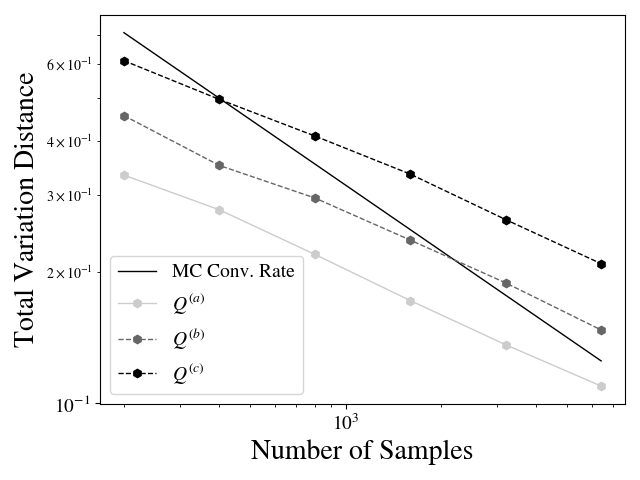
\includegraphics[width=0.45\linewidth]{./images/Plot-reg_BigN_8000000_reg_M_1_rand_I_100000.png}

\caption{The results of $d^2_\text{TV}(\PP_{\pspace, \ndiscs, \nsamps}, \PP_{\pspace, \ndiscs, \bar{\nsamps}})$ for $\ndiscs = 1, \bar{\nsamps} = 8,000,000$, with $a, b, c = 1, 2, 4$ in three dimensions.}
\label{fig:M1_3d}
\end{figure}
\FloatBarrier
In Figure~\ref{fig:M1_3d}, it appears that the effect of skewness is even more pronounced in higher dimensions, and that the number of samples required to achieve similar levels of accuracy between two maps with a ratio of skewness 2 is now quadrupled.
The analysis of \cite{BGE+15} suggested a dependence of accuracy related to the skewness raised to a power related to the dimension of the data space.

%%%%%%%%%%%%%%%%%%%%%%%%%%%%%%%%%%%%%%%%%%%%%%%%%%%%%%%%%%%%%%

\section{Accuracy of Sample-Based Inversion}\label{sec:ch03-sample}

How does the new approach compare? What role does the KDE play in the error?
Focus on linear problems. One or two examples (perhaps use that skew-map with 1 and 2 and 4).

%%%% Sample-Based Skewness Example %%%%%%

\subsection{A Sample-Based Solution}\label{eq:sampleskew}

Here we solve the problems in Examples~\ref{ex:skewness} and~\ref{ex:3dmap}, except in the framework of the Sample-Based Inversion outlined in \ref{sec:ch02-sample}.
Effect of Skewness appears to be mitigated.
\vfill{10in}

%%%%%%%%%%%%%%%%%%%%%%%%%%%%%%%%%%%%%%%%%%%%%%%%%%%%%%%%%%%%%%

\
\section{Numerical Results and Analysis}\label{sec:ch03-examples}


We have an interest in understanding what values of $\nsamps$ would be appropriate provided we want to resolve $d(\PP_{\pspace, \ndiscs, \nsamps}, \PP_{\pspace, \ndiscs})$ to some desired level of accuracy, below some tolerance so that Equation~\eqref{eq:objective} is effectively satisfied if
\begin{equation}\label{eq:newobjective}
d(\PP_{\pspace, \ndiscs, \nsamps}, \PP_{\pspace,\ndiscs}) < \tau,
\end{equation}
where $\tau$ is some designated tolerance.

Recall that this discussion of error is in reference to some fixed $\qoi\in\qspace$ to which Algorithm~\ref{alg:inv_density} is applied.
The inequality presented in Eq.~\eqref{eq:set-triangleineq} holds for probability measures induced by any map in $\qspace$, though we obscure the dependence on $\qoi$ for the time being.
To this end, we introduce notation of the form $\PP_{\pspace, \ndiscs, \nsamps}^{\qoi}$ when we want to distinguish between measures constructed from inverting a particular map $\qoi\in\qspace$.

The reason for this is because as the work of (cite: Butler AWR) has shown, the choice of $\qoi$ will influence the number of model solutions necessary to accurately solve the SIP.
Different choices for $\qoi$ may lead to radically different values for $\nsamps$ in order to achieve the same bound on $d(\PP_{\pspace, \ndiscs, \nsamps}, \PP_{\pspace, \ndiscs})$, and it is the goal of this work to explore this relationship.

The analysis of this problem differs significantly from the ones in (cite: butler, mattis), which bound errors in probability of estimating sets $A\in\pborel$.
By phrasing our analysis in terms of metrics (discussed more in Section~\ref{sec:metrics}), we may be able to answer more broadly generalizable questions about error, including those regarding convergence rates and global accuracy of our estimates.


Total Variation\subsection{Example: Thermal Conductivity on a 1D Heat Rod}\label{ex:heat-set-sample-accuracy}

Consider the one-dimensional heat equation with homogeneous Neumann boundary conditions on the unit interval presented in \ref{ex:heat-set-sample}.


The quantities of interest we study are four point-evaluations of the state variable, at spatial location 0.25, 0.51, 0.67, and 0.98 along the rod.
Choosing any pair of them for the inversion yields six possible quantities of interest maps.
As before, we demonstrate that some choices appear to have advantages over others.

From the prior examples, we would suspect that choosing the QoI map with lower skewness results in lower Total Variations.
However in the earlier experiments we utilized maps that inverted into sets of identical size, which is not the case in this nonlinear example; each QoI map scales sets differently depending on the location in the parameter space.
To isolate this scaling effect, we attempt to compare QoIs that invert into sets of similar size \emph{on average} but have differing average skewness.

This is what motivated our specific choice of spatial locations at which to measure the state variable $T$.
Our first QoI $\qoiA$ uses measurements at 0.25 and 0.51, and has average skewness of 1.08, and our second $\qoiB$ uses measurements at 0.67 and 0.98, with average skewness 1.56.
While we would have liked to use a map with average skewness of 2 for a more similar comparison to the prior examples, this was the best range we could find where the maps inverted into sets of comparable size on average\footnote{average local scaling is 1.99 versus 2.19}.

Owing to the nonlinearity of the problem, the Total Variations between reference and estimated probability measures now have an inherent dependence on the location of the point $\param$ in the parameter space.
We ran the simulations for a regular $3\times3$ grid exploring the interior of the parameter space and present a selection of two reference points that illustrate the differences in the nonlinear case.

In the two-dimensional data spaces $\dspaceA$ and $\dspaceB$, our uncertainty is a uniform box centered at $\qoiA(\paramref)$ with side-lengths of 0.1.
When $\paramref$ is the bottom-left corner of our $3\times3$ grid, the two maps produce very different results, with $\qoiA$ outperforming $\qoiB$ in a similar manner as we saw in the linear examples (see Fig.~\ref{fig:NLbotleft}).
When $\param_{\text{ref}}$ is in the upper-center of the grid, the inverse images are similar, as shown in Fig.~\ref{fig:NLtopmid}, and so which map to use forinversion into this part of the parameter spaces is not a clear choice. We might even be tempted to use the more-skewed (on average) map since it inverts into a set with smaller support.


\begin{figure}[h]
\begin{minipage}{.475\textwidth}
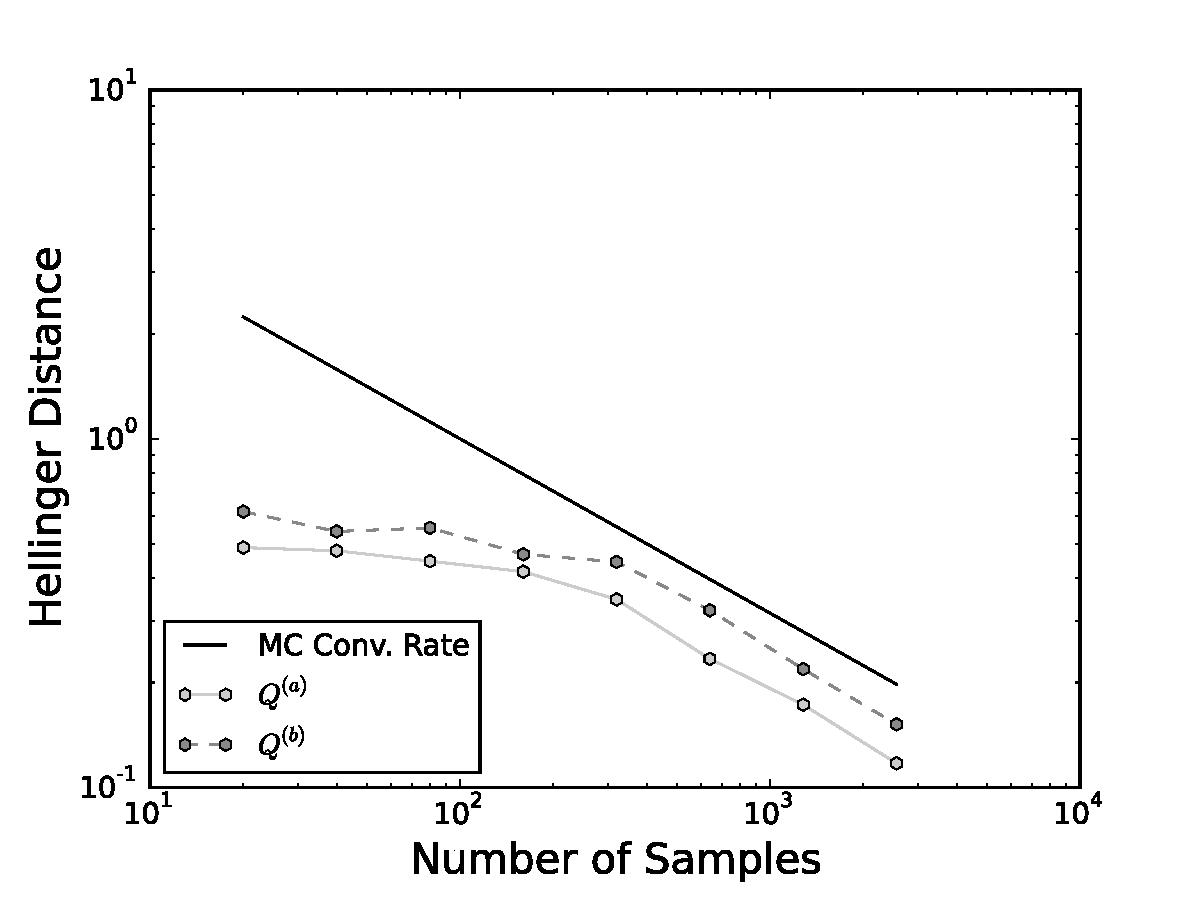
\includegraphics[width=\linewidth]{./images/pt0Plot-reg_BigN_40000_reg_M_1_rand_I_100000}
\end{minipage}
\begin{minipage}{.475\textwidth}
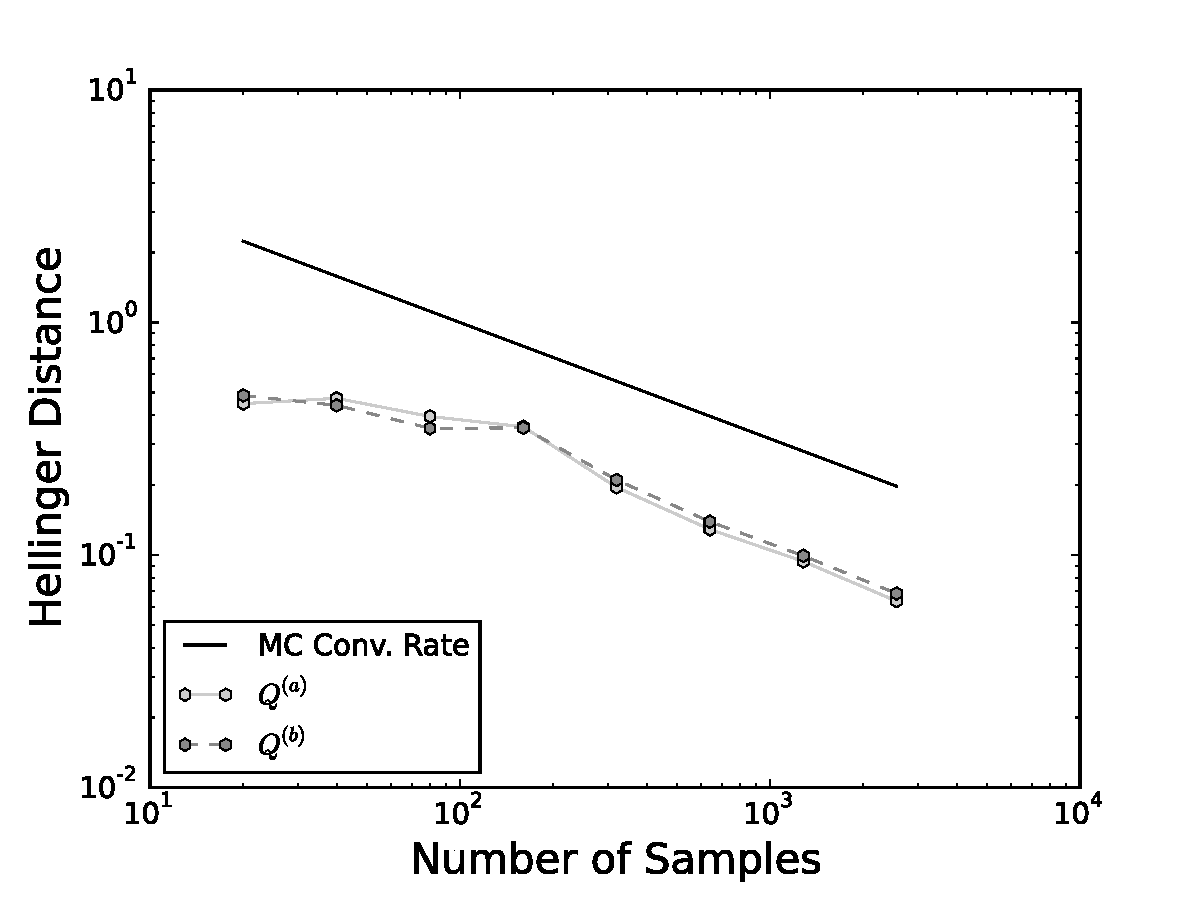
\includegraphics[width=\linewidth]{./images/pt5Plot-reg_BigN_40000_reg_M_1_rand_I_100000}
\end{minipage}
  \caption{Comparison of the differences in Total Variations for the two maps and two reference points. The results for the bottom-left reference value is shown on the left and the top-center is shown on the right.}
\label{fig:NLHD}
\end{figure}

The Total Variation plots for these two reference values are compared in Fig.~\ref{fig:NLHD}.
Of the nine reference $\param$'s we studied, $\qoiA$ yielded no considerable advantage in terms of the number of samples required to approximate the inverse images in three cases (the plots were similar to that in the right of Fig.~\ref{fig:NLHD}).
In three cases, $\qoiA$ performed just a bit better than $\qoiB$, (somewhere between the two figures in Fig.~\ref{fig:NLHD}).
In two cases, $\qoiA$ performed better than  $\qoiB$, as in the left of Fig.~\ref{fig:NLHD}.
In one case (with $\param$ in the bottom right corner), the difference was even more dramatic ($\qoiA$ yielded similar Total Variations with less than a fourth the samples).

\begin{figure}
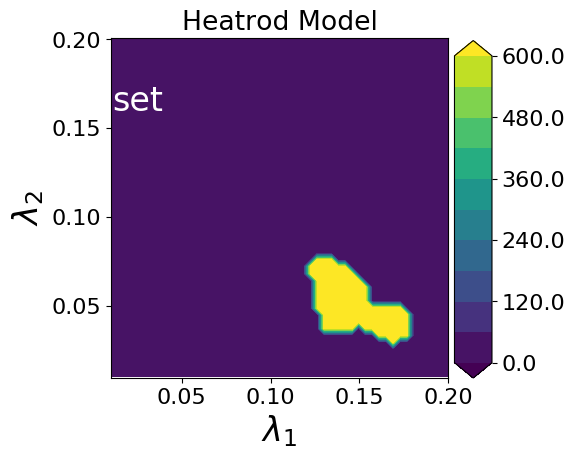
\includegraphics[width=.45\linewidth]{examples/fig_heatrod_q1/HeatrodModel--set_N50_em.png}
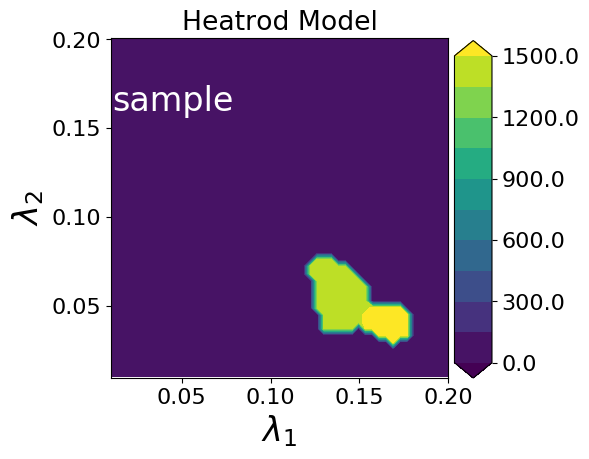
\includegraphics[width=.45\linewidth]{examples/fig_heatrod_q1/HeatrodModel--sample_N50_mc.png}

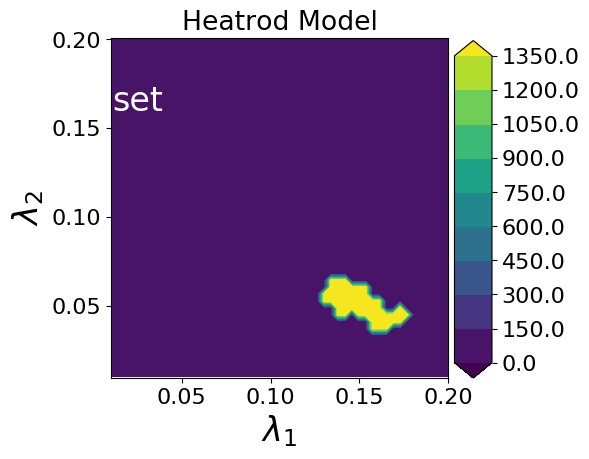
\includegraphics[width=.45\linewidth]{examples/fig_heatrod_q1/HeatrodModel--set_N500_em.png}
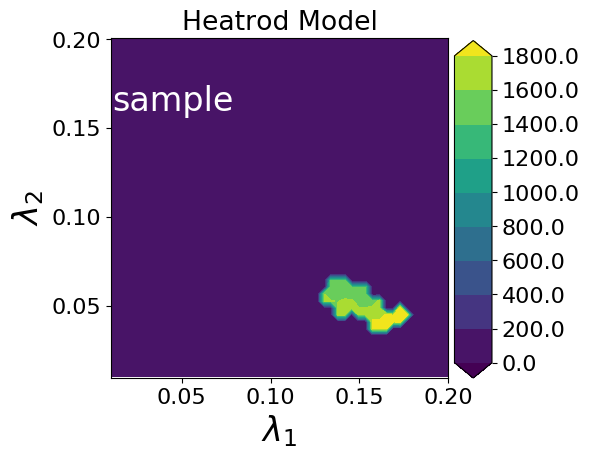
\includegraphics[width=.45\linewidth]{examples/fig_heatrod_q1/HeatrodModel--sample_N500_mc.png}

\caption{The inverse image of the reference measure for $\qoiA$ for $\nsamps = 50$ (top) and $\nsamps = 500$ (bottom). }
\label{fig:heatrod-convergence-a}
\end{figure}

\begin{figure}
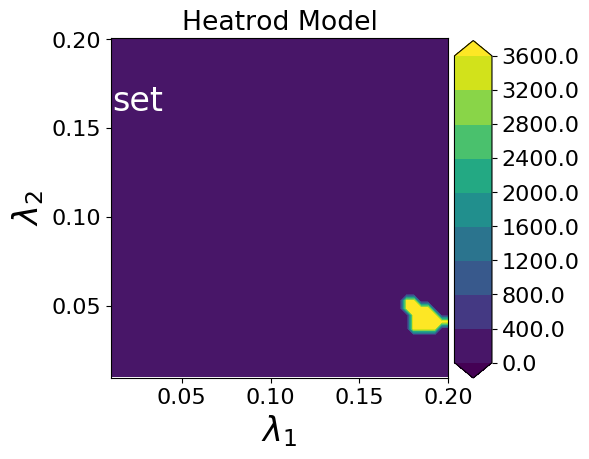
\includegraphics[width=.45\linewidth]{examples/fig_heatrod_q2/HeatrodModel--set_N50_em.png}
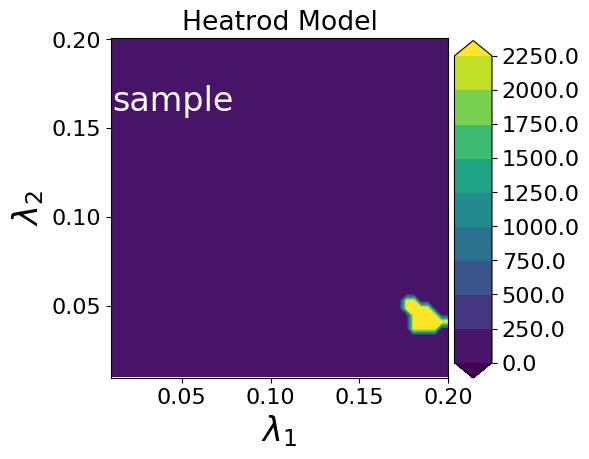
\includegraphics[width=.45\linewidth]{examples/fig_heatrod_q2/HeatrodModel--sample_N50_mc.png}

\includegraphics[width=.45\linewidth]{examples/fig_heatrod_q2/HeatrodModel--set_N500_em.png}
\includegraphics[width=.45\linewidth]{examples/fig_heatrod_q2/HeatrodModel--sample_N500_mc.png}

\caption{The inverse image of the reference measure for $\qoiB$ for $\nsamps = 50$ (top) and $\nsamps = 500$ (bottom). }
\label{fig:heatrod-convergence-b}
\end{figure}

With these nonlinear cases, we find that taking an ``on average'' approach is inefficient, as there can be dramatic differences in the geometric properties of the inverse images in the parameter space depending on the location.
These results motivate further study into utilizing different QoI maps (perhaps some of those other four combinations available to us in this example) depending on where the samples came from in the parameter space.
In general, we saw in this example that given that two maps invert into sets of similar size on average, using the one with lower skewness results in less samples required to accurately approximate the inverse image.
The maps we used had average skewnesses that differed by 0.5 (instead of by 1), and the trend from the linear examples still held in significant portions of the parameter space.

\FloatBarrier

\subsection{Example: Initial Condition and Rate of Something Decaying}\label{ex:decay-set-sample-accuracy}

\begin{figure}[h]
\begin{minipage}{.4\textwidth}
\includegraphics[width=\linewidth]{examples/fig_decay_q1/DecayModel--set_N50_em.png}
\includegraphics[width=\linewidth]{examples/fig_decay_q1/DecayModel--set_N500_em.png}

\includegraphics[width=\linewidth]{examples/fig_decay_q2/DecayModel--set_N50_em.png}
\includegraphics[width=\linewidth]{examples/fig_decay_q2/DecayModel--set_N500_em.png}
\end{minipage}
\begin{minipage}{.4\textwidth}
\includegraphics[width=\linewidth]{examples/fig_decay_q1/DecayModel--sample_N50_mc.png}
\includegraphics[width=\linewidth]{examples/fig_decay_q1/DecayModel--sample_N500_mc.png}

\includegraphics[width=\linewidth]{examples/fig_decay_q2/DecayModel--sample_N50_mc.png}
\includegraphics[width=\linewidth]{examples/fig_decay_q2/DecayModel--sample_N500_mc.png}
\end{minipage}

\caption{The inverse image of the reference measure for $\qoiA$ (top half) and $\qoiB$ (bottom half). }
\label{fig:decay-convergence}
\end{figure}

With these nonlinear cases, we find that taking an ``on average'' approach is inefficient, as there can be dramatic differences in the geometric properties of the inverse images in the parameter space depending on the location.
These results motivate further study into utilizing different QoI maps (perhaps some of those other four combinations available to us in this example) depending on where the samples came from in the parameter space.
In general, we saw in this example that given that two maps invert into sets of similar size on average, using the one with lower skewness results in less samples required to accurately approximate the inverse image.
The maps we used had average skewnesses that differed by 0.5 (instead of by 1), and the trend from the linear examples still held in significant portions of the parameter space.

\FloatBarrier
%%%%%%%%%%%%%%

\FloatBarrier

\chapter{\uppercase{Extensions and Applications of MUD Points and Skewness Analysis} \label{chapter:vector-valued}}

In Chapter~\ref{chapter:geometry}, we introduced the notion of skewness and showed examples of how it impacts the accuracy of approximating SIP solutions with finite sampling.
Here, we demonstrate how an awareness of skewness allows us to a priori define a QoI that will\---on average\---better resolve $\paramref$ by providing information in mutually distinct directions in $\pspace$.
We begin by revisiting the example in Section \ref{subsec:pde-example} involving the Poisson problem and uncertain Neumann boundary condition $g$.
Recall that $\qoi_\text{2D}$ is able to better resolve $\paramref$ than $\qoi_\text{1D}$.
The map $\qoi_\text{2D}$ is presented as an alternative option for aggregating the same one hundred measurements and using them to construct a more informative 2D map.
In this chapter, we present a more detailed study of the construction of this map, and perform a case-study in designing a problem where the data-constructed QoI map is more informative.


We demonstrate how an awareness of skewness can allows us to define a QoI a-priori that will\---on average\---better resolve $\paramref$ by providing information in mutually distinct directions in $\pspace$.
We begin by revisiting the example in Section \ref{subsec:pde-example} involving the Poisson problem and uncertain boundary condition $g$.
Recall how $\qoi_\text{2D}$ was able to better resolve $\paramref$ than $\qoi_\text{1D}$.
The map $\qoi_\text{2D}$ was presented as an option for taking the same available hundred measurements and using them to form a more informative map.
In this chapter, we present a more detailed study of the construction of this map, reflecting a case-study in designing a problem where the QoI map is informative.

\section{Extension to Vector-Valued QoI Maps}
In our first example, we show that a small change in the decision of how to partition the measurements collected on the response surface can induce a 2-dimensional map $\qoi_\text{2D}^\prime$ which is ``effectively'' one-dimensional in that the two components provide highly correlated information.
Such a map is more skewed than the one we presented with $\qoi_\text{2D}$, and so leads to MUD-point solutions that exhibit similar behavior to those that we got when we used $\qoi_\text{1D}$ in the original problem.
This decreased precision demonstrates that skewness\---although developed in the previous chapter within the context of set-valued solutions\---is still a relevant measure of a map's utility when solving parameter identification problems.

The examples in Sections~\ref{subsec:ode-example} and \ref{subsec:pde-example} motivate the use of a data-constructed QoI in order to incorporate an arbitrary number of measurements in a system into a scalar-valued map.
These examples were chosen so that $\text{dim}({\Lambda}) = 1$ for simplicity and to establish a baseline for convergence results.
The linear examples in Section~\ref{sec:high-dim-linear-example} demonstrate that the DCI framework maintains the accuracy of least-squares while incorporating initial beliefs for higher-dimensional linear maps.
In those examples, we showed that our ability to resolve a true parameter improved as the gap between input dimension and operator row-rank shrunk.

The rank-deficiency of an operator can be attributed either to ill-conditioning of an operator $A:P\to P$, or when $P>D$ for a full-rank $A:P\to D$.
In scenarios where $S>P$ observations are available, we are motivated to somehow leverage the form of Eq.~\eqref{eq:qoi_WME} to construct a vector-valued version incorporating subsets of $S$ for each component.
For example, a system for which spatial measurements are available over time may motivate constructing a scalar-valued WME map for each spatial location.
If distinctly different observable quantities are available (ones perhaps with different physical units), then these may be collapsed into each component of the map.

The discussion of how to optimally construct such maps is beyond the scope of this work, and would need to take into account nuances involving measurement sensitivities and address combinatorial design-spaces.
However, we summarize that the extension of the equations presented in Section~\ref{sec:MUD_analysis} follows directly by constructing the resultant $1\times P$ matrices $A$ and scalar-valued $b$ for each component and then stacking them to form a $D\times P$ system, where we are motivated to minimize $P-D$.

%%%%%%%%%%%%%%%%%%%%%%%%%%%%%%%%%%%%%%%%%%%%%%%%%%%%%%%%%%%%%%%%%%%%
%%%%%%%%%%%%%%%%%%%%%%%%%%%%%%%%%%%%%%%%%%%%%%%%%%%%%%%%%%%%%%%%%%%%

% \subsection{A Vector-Valued QoI Map}
% In the PDE example of \ref{sec:pde-example}, we presumed knowledge about the structure of $g$ being a sine curve; we only had to estimate a scaling coefficient for it.
% To demonstrate the use of the WME QoI in solving inverse problems in higher dimensions, we set up the following series of examples in the same spirit with respect to the model and measurement locations, but presuming less about $g$ than before.
%
% We choose a polynomial function $g$ which exhibits similar behavior to the former sine curve, but without the symmetry about $x_2=0.5$, and scale it so that it takes a minimum at the same value as before (at $g = -3$).
% We selected $g(x) = \alpha x_2^2 (x_2 - 1)^5$, with $\alpha$ chosen to satisfy the aforementioned design specification (so that $g(x)=-3$ for $x=(0,\frac{2}{7})$).
% Suppose that as modelers, we are told only that $g$ is negative and bounded below by $-4$.
%
% We propose beginning to estimate it by placing two knots on the interior of the domain of $g$ and trying to deduce its value at these points.
% This gives us a parameter space of $\pspace = [-4, 0]$, and over this space we will assume a uniform density again.
% Our first two knots will be the equispaced points $x = (0,\frac{1}{3}), (0,\frac{2}{3})$, and the family of functions that this spans is visually illustrated in the left half of Figure~\ref{fig:pde-highd-initial-2d}.
% We also plot the true function and the associated piecewise--linear that comes from interpolating the true $g$.
% Observe that none of these (purple) functions we are considering to explain the data we collected (from the black curve) really adequately capture the correct dynamics, and that even the piecewise-linear interpolant (red) mis--characterizes the true boundary condition for most of the domain.
%
% The rest of the problem setup will be kept the same as the previous example, except that instead of $N=10,000$ parameter space samples, we use $N=1,000$.
% The reason for this is that we will not be doing the same convergence studies, so we are less interested in exhaustively exploring $\pspace$ than demonstrating that our method can handle a wider variety of inverse problems than the previous examples may suggest.


%
% \subsubsection{A Scalar-Valued QoI Map}
%
% Our first inverse problem involves solving the SIP with the same scalar-valued QoI map constructed by incorporating all the measurements into \eqref{eq:qoi_WME}.
% To give the reader a sense of the ability for this ``basis'' to match the one-hundred measurements used for inversion, we plot the best match of our thousand parameter samples with respect to these measurements in purple in the top half of Figure~\ref{fig:pde-highd-2d-projection}.
% There, we also plot the closest match to the interpolating piecewise-linear function in green, and note that we have a near-identical match among our thousand parameter samples, though the best predictor of the data we collected is a different sample.
% We are curious which of these two functions the MUD will more closely resemble.
% The residual Q-Q plots for the two functions are shown to illustrate the differences in misfit to provide an alternative view to the goodness-of-fit.
%
%
% \begin{figure}
% \centering
%   \includegraphics[width=0.95\linewidth]{figures/pde-highd/pde-highd_proj_D2.png}
% \caption{ TK - x-axis label needs to be fixed and this figure needs a proper caption.
% }
% \label{fig:pde-highd-2d-projection}
% \end{figure}
%
%
% In the bottom half of \ref{fig:pde-highd-2d-scalar-mud}, we show the MUD solutions arising from twenty trials using different observations of noise.
% Of particular interest is that the solutions seem to discover one of two types of explanations for the data, seemingly unable to decide which half of the domain represents a better estimate of $g$'s minimum value.
% As mentioned, this set of solutions comes from collapsing all hundred measurements into a scalar--valued QoI map, which negatively impacts our ability to identify the parameter in the problem, since our SIP is now $2\rightarrow 1$.
% [TK - cite Troy's result about dimensions from AWR paper] implies that we have an incentive to construct maps which ``close the gap,'' so to speak, between input and output dimension, to fully leverage the geometry of available information.
% The contour structure of the updated density samples plotted in red in \ref{fig:pde-highd-2d-example}.
%
% \begin{figure}
% \centering
%   \includegraphics[width=0.95\linewidth]{figures/pde-highd/pde-highd_pair_D2-1_m100.png}
% \caption{ TK - x-axis label needs to be fixed and this figure needs a proper caption.
% }
% \label{fig:pde-highd-2d-scalar-mud}
% \end{figure}

\FloatBarrier
\subsection{Skewness and Vector-Valued QoI Maps}

Suppose that instead of constructing a scalar--valued QoI map, we used the form of \eqref{eq:qoi_WME} to construct a map with two components, yielding a $2 \rightarrow 2$ SIP instead.
We saw how such an approach could provide any tangible benefit for resolving the uncertainty in our true function $g$ in \ref{subsec:pde-example}, but presented the map $\qoi^{2D}$ without discussion of how it was selected.
To explore the impact of our choices in how $\Omega$ was partitioned into components of a QoI map, we propose two methods for splitting our hundred measurements into two subsets, which will be used to construct the respective components of the map according to \eqref{eq:qoi_WME}.
Both methods are shown in the top half of Figure~\ref{fig:pde-highd-2d-geometry}, and represent a bisection through $\Omega$ vertically and horizontally.

\begin{figure}
\centering
  \includegraphics[width=0.475\linewidth]{figures/pde-highd/pde-highd_sensors_D2.png}
  \includegraphics[width=0.475\linewidth]{figures/pde-highd/pde-highd_sensors-alt_D2.png}
  \includegraphics[width=0.95\linewidth]{figures/pde-highd/pde-highd_geom_D2.png}
\caption{
(Bottom): The vector-valued QoI map is constructed for all $N=10,000$ parameter evaluations and the two resulting vectors are plotted against one another for both methods of partitioning $\Omega$.
}
\label{fig:pde-highd-2d-geometry}
\end{figure}

We now highlight our approach to addressing the following question:

\begin{centering}
\emph{With two QoI maps under consideration, which should we use?}
\end{centering}

Before solving an inverse problem, there are a priori analyses that can be performed that can provide heuristics to help address these questions.
We first evaluate our thousand parameter samples through each of these maps and inspect the two-dimensional scatter-plots to build intuition about the underlying geometry induced by these maps.
We repeat this process for three subsets of the measurements (using the first samples in each half of $\Omega$ according to the random index assigned to them), and demonstrate the two resulting sets of relationship in the bottom half of Figure~\ref{fig:pde-highd-2d-geometry}.
This figure also shows the associated designs against the noisy response surface as a backdrop.

First, we note that the inclusion of more data points has the effect of dilating (and to some extent rotating) the induced data space for both QoI maps.
The geometric implication of this in the context of the chosen form of the QoI map has an interesting consequence.
Recall that the observed distribution remains a standard Gaussian, regardless of the number of data points used to construct the map.
In two dimensions, this observed distribution becomes a multivariate normal distribution instead, which can be visually thought of as a circular ``target'' located in the middle of each of the scatter-plots in Fig. \ref{fig:pde-highd-2d-geometry}.
As more measurements are incorporated, the size of that target relative to the rest of the space becomes increasingly small since the data manifolds dilate.
It is akin to finding the same needle in larger piles of hay.
More is asked of the solution to the SIP, since there are more measurements with which the model must agree.

The second implication of the two ways in which the maps can be formed is more visually evident, as the two quantities of interest that arise from a vertical bisection of $\Omega$ are nearly perfectly correlated.
The two maps are presenting almost the same information (the shapes are very slim parallelograms), and so we fundamentally can already expect there to be very little difference between MUD points arising from using this map when compared to using the scalar--valued map.
Particularly since the observed distribution is radially symmetric, this problem\---while technically two-dimensional\---appears to be one-dimensional.

By contrast, the map induced by a horizontal split (bottom left of Fig. \ref{fig:pde-highd-2d-geometry}) provides new information in each component.
While there is some correlation (the manifolds are not rectangular), a far greater proportion of samples will fall within the practical support of the observed distribution, which qualifies them as possible solutions to the SIP.
More information is learned with the inclusion of each component using this design than would be with the vertical split.

To this end, for the sake of brevity, we focus our attention on comparing the horizontal vector--valued QoI map to the scalar one, and note that a more fulfilling discussion of constructing QoI maps that induce desirable geometric properties is of interest for future work.
For the remainder of this example, the ``vector--valued'' map will refer to the the one which is split horizontally, and we note that this design, while not guaranteeing optimality for precision or accuracy's sake, at least respects the flow of information in the system being studied.
Since $\param$ is parameterizing the left Neumann boundary condition, information about its state flows from left to right in the horizontal direction.

%%%%%%%%%%%%%%%%%%%%%%%%%%%%%%%%%%%%%%%%%%%%%%%%%%%%%%%%%%%%%%%%%%%%
%%%%%%%%%%%%%%%%%%%%%%%%%%%%%%%%%%%%%%%%%%%%%%%%%%%%%%%%%%%%%%%%%%%%
\FloatBarrier
%%%%%%%%%%%%%%%%%%%%%%%%%%%%%%%%%%%%%%%%%%%%%%%%%%%%%%%%%%%%%%%%%%%%
%%%%%%%%%%%%%%%%%%%%%%%%%%%%%%%%%%%%%%%%%%%%%%%%%%%%%%%%%%%%%%%%%%%%
\section{Extension to Higher Dimensions}

Suppose now that an eager experimenter decided to start with a five--dimensional problem (five knots to describe $g$ instead of two), trying to accomplish greater granularity in the ability to estimate $g$, and imposes the same type of uniform initial density in each direction, yielding a parameter space of $\Lambda = [-4, 0]^5$.
In Figure~\ref{fig:pde-highd-initial}, we show what such initial functions would look like, and note that many of them appear to exhibit fluctuating behavior for which the mesh ($36\times36$) being used to solve the problem, would not be fine enough to resolve.
In many senses, this choice of initial density induces a lot of noise into the SIP we are hoping to solve, since ``common sense'' from a modeler's perspective.
One may be able to rule out zig-zag functions from wasting a model-evaluation budget, which we fix at the same $N=1000$ samples as in the previous 2-D problems.
To get a sense of what the best possible representations in this peculiar choice of ``basis'' could be, we again find the closest match to the interpolant and to the data and plot them alongside residuals in Figure~\ref{fig:pde-5d-proj}.

\begin{figure}
\centering
  \includegraphics[width=0.475\linewidth]{figures/pde-highd/pde-highd_init_D5.png}
\caption{
One thousand initial parameter samples (our model evaluation ``bugdet'') were used to estimate $g$, constructed by taking independent uniform samples from $[-4, 0]$ for each direction are shown in purple.
}
\label{fig:pde-highd-initial-5d}
\end{figure}


\begin{figure}[htbp]
\centering
  \includegraphics[width=0.675\linewidth]{figures/pde-highd/pde-highd_proj_D5}
\caption{
}
\label{fig:pde-5d-proj}
\end{figure}

Observe that in Figure~\ref{fig:pde-5d-proj}, both the closest fit in parameter and measurement space fail to resolve the true function behavior at $\lambda_5$ (the interpolating piecewise--linear is shown again for reference), and both place a minimum at $\lambda_2$.
The lines here are in some sense, the best that can be solved for with this design, and is helpful for comparing against our MUD solutions.
Of particular interest is that both functions under-estimate $g$ at $\lambda_2$ by a large margin.
Nevertheless, we pursue the solution for demonstration purposes and solve the SIP for both scalar-- and vector--valued QoI maps, the latter constructed with horizontal bands shown in the bottom left of Figure \ref{fig:pde-highd-5d-example}.

\begin{figure}[htbp]
\centering
  \includegraphics[width=0.95\linewidth]{figures/pde-highd/pde-highd_surf_exmud_D5_m100}
  \includegraphics[width=0.35\linewidth]{figures/pde-highd/pde-highd_sensors_D5}
  \includegraphics[width=0.6\linewidth]{figures/pde-highd/pde-highd_comp_exmud_D5_m100}
\caption{
(Top): Layout for 5-D vector--valued map and comparison of the two MUD solutions in parameter space.
(Bottom): The response surfaces predicted by the two QoI maps alongside the noisy response surface that generated the simulated collected data.
}
\label{fig:pde-highd-5d-example}
\end{figure}

In Figure~\ref{fig:pde-highd-5d-example}, the scalar-- and vector--valued MUD solutions are shown for the noisy surface plotted in the top-center, with associated predicted response surfaces flanking it.
In the bottom-center plot, we can see that the scalar-valued MUD completely misidentifies the location of $g$'s minimum value, but the vector-valued QoI is able to resolve the behavior much better.
In Figure~\ref{fig:pde-highd-5d-mud} we plot the results from twenty repeated trials (perturbations of noise) when using all hundred measurements, and observe the same difference in going from scalar-- to vector--valued solutions for the five--dimensional example that we saw in two dimensions with \ref{fig:pde-highd-2d-scalar-mud}\footnote{See Appendix (???) for examples of the twenty MUD-solutions using different numbers of measurements.}

\begin{figure}[htbp]
\centering
  \includegraphics[width=0.95\linewidth]{figures/pde-highd/pde-highd_pair_D5-1_m100}
  \includegraphics[width=0.95\linewidth]{figures/pde-highd/pde-highd_pair_D5-5_m100}
\caption{
(Top): Scalar-valued solutions.
(Bottom): Vector-valued solutions.
}
\label{fig:pde-highd-5d-mud}
\end{figure}

By increasing the number of quantities of interest used, more directions of uncertainty are resolved in the parameter space.
Since any solution in the equivalence class is valid for the SIP, the scalar-valued solutions are significantly more sensitive to noise, and so the solutions often appear to identify functions with a minimum on the wrong half of the spatial domain.
In the left half of Figure~\ref{fig:pde-highd-5d-mud}, the scalar-valued QoI is unable to differentiate between resolving residual discrepancies in different locations in $\Omega$.
By contrast, the vector-valued QoI shown below it is again constructed with respect to the flow of information in the system, and so many more of the twenty trials land closer to the true minimum value of $g$.
The solutions for the vector-valued approach instead explore the available knots (at $x_2=1/6$ and $1/3$), nearest the actual minimum value of $2/7$ instead, a much more valuable area of $\Lambda$ to explore.

Perhaps unsurprisingly given the poorly-designed initial density, our MUD solutions still do not really trace out the interpolants or projections from Fig~\ref{fig:pde-5d-proj} that we hope it should in order to approximate $g$.
At the very least, we would hope to accurately estimate the location and value of $g$'s minima.
Recall from the theory in \ref{subsec:nonlinear-example} that we previously solved a two-dimensional version of this problem, which could have been used to inform a much smaller region of two of the five directions to explore.
We now explore what would happen if our initial density was constructed with more care (without needing to use any model evaluations), since we saw from earlier examples that if DCI is initialized at a good initial mean, it has a chance of outperforming least-squares solutions in resolving discrepancy in truth.

%%%%%%%%%%%%%%%%%%%%%%%%%%%%%%%%%%%%%%%%%%%%%%%%%%%%%%%%%%%%%%%%%%%%
%%%%%%%%%%%%%%%%%%%%%%%%%%%%%%%%%%%%%%%%%%%%%%%%%%%%%%%%%%%%%%%%%%%%

\subsection{Alternative Experimental Approach}

As we proceed from two to five dimensions, being weary of the fact that we are fighting against the curse of dimensionality, we want to be more intelligent with our specification of an initial density.
Let us take a look at the samples that show up in black on the right of Figure~\ref{fig:pde-highd-2d-scatter} from a different perspective.
These represent samples from the updated density solved by incorporating all thousand measurements.
Instead of looking at high-probability samples as locations in $\pspace$, let us inspect them as a family of functions that are defined on the unit interval and use the envelope curves they sweep out to inform the specification of a better initial density; consider Figure~\ref{fig:pde-highd-5d-study}.

\begin{figure}[htbp]
\centering
  \includegraphics[width=0.675\linewidth]{figures/pde-highd/pde-highd-alt_initial_D5_m100.png}
\caption{
By considering the relationship between the parameters and the types of functions that could be possible given the solution to a 2-D inverse problem, we are able to create a more restricted parameter space in 5-D.
Knowledege of the behavior of $g$ at the boundaries allows for more than half of each of the three remaining intervals to be ruled out as infeasible regions when we look at high-probability samples from the 2-D SIP solution.
}
\label{fig:pde-highd-5d-study}
\end{figure}

The samples whose relative ratios exceeded $1/1000$ sweep out a family of curves that can be used to estimate bounds not only on $\lambda_2$ and $\lambda_4$ (the previous $\lambda_1$ and $\lambda_2$ from the 2-D problem)\---which exhibit correlation structure that we will turn to momentarily\---but also on the remaining three knots.
To form the intervals shown in orange in Fig.~\ref{fig:pde-highd-5d-study}, we take the upper and lower bounds of the curves passing through the vertical lines drawn at the three new knot values.
To be conservative, we multiply our lower bound by $1.2$ and the upper by $0.8$.
With these choices, we are still more than halving the interval-length in each direction as compared to the previous 5-D problem.
(Alternatively, one could establish a lower tolerance for accepting likely samples and avoid the multiplication factor, but a thorough exploration of how to best leverage the ratio of observed to predicted densities is left to future work.


\FloatBarrier
\subsubsection{A Better Initial Density}
For the two remaining directions, we want to capture the correlation structure that we were able to visually identify in Fig.~\ref{fig:pde-highd-2d-example} and impose something uniform-ish on it.
To achieve this, we perform a singular-value decomposition on the likely samples from the \emph{scalar}--valued 2-D solution, since there are so many more samples\footnote{ The scalar-valued contour was found to better characterize the direction of the equivalence class, suggesting perhaps a justifiable use for solving the problem with it. We could have formed an estimate of the updated density from using the vector--valued QoI and sampled from that instead. Many such approaches can be looked into in the future and are briefly discussed in the last section of this chapter.}.
The singular vectors are used to transform the vector-valued samples, and a uniform sampling is performed over the rectangular bounding box for these points, shown in the center of Figure~\ref{fig:pde-highd-2d-study}.
These generated samples, however, leave $\pspace$ when transformed back to their native space, as seen in the left panel.
To ameliorate this problem, we instead perform sampling in a while-loop, sampling from this uniform box and rejecting any that would get mapped back outside $\pspace$, until we reach our desired thousand samples.


\begin{figure}[htbp]
\centering
  \includegraphics[width=0.95\linewidth]{figures/pde-highd/pde-highd-alt_initial_D2_m100}
\caption{
Generating proposal samples for the two directions informed by solving the 2-D inverse problem, aided by singular-value decompositions and an ad-hoc sampling procedure.
}
\label{fig:pde-highd-2d-study}
\end{figure}

Furthermore, note that in the center panel of Fig~\ref{fig:pde-highd-2d-study}, there are corner-regions of the space we want to avoid wasting samples on as well, so we reject samples that have squared two-norm greater than $0.05$ from their nearest vector--valued sample.
This sampling procedure produces the set shown in orange on the right side of the figure (ten thousand shown to demonstrate coverage).
In a sense, we set out to define a computational open cover for the relatively high-probability samples.
We keep one thousand of these 2-D samples, and join them with the three independent uniform sample sets of the same size taken from the intervals shown in Fig.~\ref{fig:pde-highd-5d-study} to form our new initial sample set, the functions from which generate the curves shown in Figure~\ref{fig:pde-highd-alt-initial-5d}.

\begin{figure}[htbp]
\centering
  \includegraphics[width=0.675\linewidth]{figures/pde-highd/pde-highd_init_D5-alt}
\caption{
Initial density constructed for the second attempt at the five--dimensional inverse problem, with the structure of solutions learned from the 2-D example incorporated into the selection of bounds in each direction.
}
\label{fig:pde-highd-alt-initial-5d}
\end{figure}

The new initial curves in \ref{fig:pde-highd-alt-initial-5d}\---especially when contrasted to those in Fig.~\ref{fig:pde-highd-initial-5d}\---represent a far more reasonable set of possibilities.
The slope of the functions considered now all only have a single sign change, a marked improvement over the two or three that many samples from \ref{fig:pde-highd-initial-5d} exhibited.
We note that such considerations of smoothness could be avoided by parameterizing $g$ with a basis of some sort, but that problem is beyond the scope of this work.
Another possible improvement would be to incorporate the correlation structure that is present in the three other directions, derivable from a similar SVD-based analysis of the interpolation of the 2-D predictions through the new knot locations.
However, doing so would require more visual exploration than the authors deem worthwhile to demonstrate the point they are trying to make, which is that better initial densities improve the quality of solutions.

\begin{figure}[htbp]
\centering
  \includegraphics[width=0.95\linewidth]{figures/pde-highd/pde-highd_surf_exmud_D5-alt_m100.png}
  \includegraphics[width=0.9\linewidth]{figures/pde-highd/pde-highd-alt_comp_exmud_D5_m100.png}
\caption{
100 measurements for the revised five--dimensional problem yield substantially better estimates in the eyeball norm.
}
\label{fig:pde-highd-5d-alt-example}
\end{figure}


\subsection{Moving to Five Dimensions with more caution}

We now come to the solutions that arise from solving the same five--dimensional inverse problem of interpolating the values of $g$ through equispaced knot points, with both types of maps, in Figure~\ref{fig:pde-highd-5d-alt-mud}.
The difference in comparison to the example solutions in Fig.~\ref{fig:pde-highd-5d-mud} is stark: no longer are the solutions dramatically under-estimating the local minimum of $g$.
To the extent to which they fail to adequately to do is due to the insufficient resolution of five knot points; both scalar-- and vector--valued solutions identify the same knot as being the likely minimum, and the latter solution estimates the minima well (horizontal line drawn for reference) in the bottom-right plot.

Once again, we repeat the experiment twenty times to better understand the differences in the solutions relative to possible noise that polluted our measurements.
We are able to notice some interesting patterns by looking at the curves on the left side of Figure~\ref{fig:pde-highd-5d-alt-mud}.
First, we note that going from scalar-- to vector--valued resolves a significant amount of uncertainty in $\lambda_2$, $\lambda_3$, and $\lambda_4$.
Namely the QoI map appears to stop considering curves which do not have a sufficiently low minimum value.
Second, while the vector--valued MUD solution curves appear to capture the general characteristics of $g$ well, a number of them under-estimated the value at $\lambda_5$ quite severely relative to the true value (near zero), which we saw in Figure~\ref{fig:pde-highd-5d-mud} as well.

\begin{figure}[htbp]
\centering
  \includegraphics[width=0.95\linewidth]{figures/pde-highd/pde-highd_pair_D-alt-5-1_m20.png}
  \includegraphics[width=0.95\linewidth]{figures/pde-highd/pde-highd_pair_D-alt-5-5_m20.png}
\caption{Compared to before, we're doing much better, even with less data incorporated into our QoI maps.}
\label{fig:pde-highd-5d-alt-mud-20}
\end{figure}

\begin{figure}[htbp]
\centering
  \includegraphics[width=0.95\linewidth]{figures/pde-highd/pde-highd_pair_D-alt-5-1_m100.png}
  \includegraphics[width=0.95\linewidth]{figures/pde-highd/pde-highd_pair_D-alt-5-5_m100.png}
\caption{
(Top): Scalar-valued solutions for alternative approach to the five-dimensional problem.
(Bottom): Vector-valued solutions.
Because we began with a better choice of initial density, both QoI maps resolve the residuals similarly (bottom-left), and produce qualitatively similar estimates of the response surface. We attribute this to the fact that the vector--valued samples were used to bound the space, but note the direction was informed by the scalar--valued samples.
}
\label{fig:pde-highd-5d-alt-mud}
\end{figure}
\FloatBarrier


\subsubsection{Demonstration of Reduction in Uncertainty}

As a final note on this experiment, we contrast the resulting $L^2$-errors to $g$ \footnote{derived from computational approximation with the trapezoidal rule} of these MUD solutions, to the previous two examples in Figure~\ref{fig:pde-highd-5d-hist}, to show a lineage of learning, so to speak.
With each successive problem, our uncertainty is reduced and our MUD solutions lower in variance and increase in accuracy.
Note that they appear to be moving towards a value away from zero, which represents a fixed bias (five equispaced knots can only approximate this $g$ so well).

\begin{figure}[htbp]
\centering
  \includegraphics[width=0.675\linewidth]{figures/pde-highd/pde-highd_hist_D5_t5-0E-01}
\caption{
Comparison of the 2D initial errors to the 5D ones, as well as the reduction of uncertainty that solving a SIP problem for each provides.
}
\label{fig:pde-highd-5d-hist}
\end{figure}

\FloatBarrier


%%%%%%%%%%%%%%%%%%%%%%%%%%%%%%%%%%%%%%%%%%%%%%%%%%%%%%%%%%%%%%%%%%%%
%%%%%%%%%%%%%%%%%%%%%%%%%%%%%%%%%%%%%%%%%%%%%%%%%%%%%%%%%%%%%%%%%%%%
\FloatBarrier
\subsection{Revisiting Example~\ref{subsec:pde-example}}

Recall that aggregating spatial data into two separate components on $\qoi_\text{2D}$ provided a tangible benefit for resolving the uncertainty in the true function $g$ in Example~\ref{subsec:pde-example}.
However, we did not present how the map $\qoi_\text{2D}$ was selected.
To explore the impact of various choices in how data may be aggregated into components of a QoI map, we propose two methods for splitting the measurements into two subsets to construct the respective components of the map according to \eqref{eq:qoi_WME}.
An illustration of the partitioning for both methods are shown in the top half of Figure~\ref{fig:pde-highd-2d-geometry}; a bisection of $\Omega$ into vertically-oriented halves is used to form $\qoi_\text{2D}^\prime$ and (as before), horizontal ones for $\qoi_\text{2D}$.

\begin{figure}
\centering
  \includegraphics[width=0.475\linewidth]{figures/pde-highd/pde-highd_sensors_D2.png}
  \includegraphics[width=0.475\linewidth]{figures/pde-highd/pde-highd_sensors-alt_D2.png}
  \includegraphics[width=0.95\linewidth]{figures/pde-highd/pde-highd_geom_D2.png}
\caption{
Comparison of $\qoi_\text{2D}$ (left) and $\qoi_\text{2D}^\prime$ (right).
Partitioning of $\Omega$ into the two components of each map is shown in the top half of the figure.
In the bottom half, the vector-valued QoI map is constructed for all $N=1000$ parameter evaluations using $\ndata=20, 60, \text{ and } 100$ measurements, and the two resulting component vectors are plotted against one another for both methods of partitioning $\Omega$.
}
\label{fig:pde-highd-2d-geometry}
\end{figure}

The choice of which partitioning method to use is akin to the following question:
\begin{center}
\emph{With two possible QoI maps under consideration, which should we use?}
\end{center}

We use heuristics and an understanding of skewness to help address this question.
For the data-constructed (WME) QoI map, the observed distribution for which we seek a pullback measure is fixed as a standard multivariate Gaussian, independent of the number of measurements that were used.
The initial density is also a fixed quantity, implying that any differences in the updated density will be attributed to differences in the predicted density.
To understand how the precision of the MUD estimate will change as more measurements are incorporated into the map, we visualize the data spaces induced by the WME QoI for increasing number of measurements $\ndata = 20, 60, \text{ and } 100$.

We sample the predicted data spaces using simulated spatial data associated with $1000$ parameter samples.
To build intuition about how the underlying geometry induced by these maps changes, we plot the scatter-plots representing a visualization of the associated data spaces in the bottom half of Figure~\ref{fig:pde-highd-2d-geometry}.
This figure also shows the associated designs against the noisy response surface as a backdrop.
The inclusion of more data points has the effect of dilating (and to some extent rotating) the induced data space for both QoI maps.
More work is required to find a good solution to the SIP, since there are more measurements with which the model must agree.

$\qoi_\text{2D}^\prime$ has much higher skewness than $\qoi_\text{2D}$, as is visually evident by the near-perfect correlation between its component values seen in the right plot of Fig~\ref{fig:pde-highd-2d-geometry}.
The most notable difference between the scatterplots is the difference in diameters (reference the axis labels) for each data space, a fact attributable to the difference in skewness.
The two component maps of $\qoi_\text{2D}$ contain almost the same information, so we can expect there to be little difference between MUD points arising from using $\qoi_\text{2D}^\prime$ when compared to using the scalar--valued map.
We compare these two solutions for an instance of the SIP in Figure~\ref{fig:pde-highd-2d-scalar-vs-alt}.

[TK - fix figure]
\begin{figure}
  \includegraphics[width=0.95\linewidth]{figures/pde-highd/pde-highd_geom_D2.png}
\caption{
Side-by-side comparison of an example solution to the SIP using $\qoi_\text{1D}$ (left) compared to using $\qoi_\text{2D}^\prime$, juxtaposed against a plot of $g$.
}
\label{fig:pde-highd-2d-scalar-vs-alt}
\end{figure}

By contrast, the map induced by a horizontal split (bottom left of Fig. \ref{fig:pde-highd-2d-geometry}) provides new information in each component.
While there is some correlation (the manifolds are not rectangular), a far greater proportion of samples will fall within the practical support of the observed distribution, which qualifies them as possible solutions to the SIP.
More information is learned with the inclusion of each component using this design than would be with the vertical split.
Had we performed an analysis of average skewness, we could have discovered these geometric implications without visual inspection.
Using a quantitative measure such as skewness allows us to scale the assessment to higher-dimensional parameter and data spaces.

We focus attention on comparing higher-dimensional QoI maps constructed from aggregating data separated into more horizontal bands to scalar QoI maps (as proxies for highly-skewed maps), and note that a more thorough discussion of constructing QoI maps that induce desirable geometric properties is of interest for future work.
In \ref{sec:mud-higher-dimensions} and \ref{sec:mud-pde-sequence}, the ``vector--valued'' map will refer to the one with data aggregated into separate horizontal bands.
We note that this design, while not guaranteeing optimality for precision or accuracy's sake, respects the flow of information in the system being studied.
Since the parameter represents the left Neumann boundary condition, information about its state flows from left to right in the horizontal direction.

\FloatBarrier


%%%%%%%%%%%%%%%%%%%%%%%%%%%%%%%%%%%%%%%%%%%%%%%%%%%%%%%%%%%%%%%%%%%%
%%%%%%%%%%%%%%%%%%%%%%%%%%%%%%%%%%%%%%%%%%%%%%%%%%%%%%%%%%%%%%%%%%%%
\section{Extension to Higher Dimensions}\label{sec:mud-higher-dimensions}
We now show that when the dimension of $\pspace$ is higher, the benefit from maximizing the dimension of the QoI map is even more considerable than what we observed in the two-dimensional cases, as long as we aggregate data into components of the QoI map in a purposeful manner.
In the first example, we demonstrate the impact of increasing the volume of the parameter space while fixing all other attributes of the inverse problem.
In the second example, we illustrate how we could utilize the solution to the SIP for the two-dimensional case from \ref{subsec:pde-example} to improve the MUD estimate in five dimensions.

\subsection{A SIP with a Naive Initial Density}
Consider a naive implementation in five dimensions, where the same prior knowledge on the bounds of $g$ inform the choice of a parameter space.
Suppose $\pspace$ is given by $[-4, 0]^5$, induced by five regularly-spaced knot points in the interior of $x_2 \in (0,1)$ for which a uniform density is assumed in each component.
In Figure~\ref{fig:pde-highd-initial-5d}, we show what one-thousand such initial functions look like, and note that many of them appear to exhibit fluctuating behavior which may require a finer mesh than the one being used to solve the problem ($36\times36$), in order to reduce numerical errors.
This choice of initial density induces a lot of ``conceptual'' noise into the SIP, since ``common sense'' from a modeler's perspective could rule out functions which zig-zag excessively.

\begin{figure}
\centering
  \includegraphics[width=0.475\linewidth]{figures/pde-highd/pde-highd_init_D5.png}
\caption{
One thousand initial parameter samples (our model evaluation ``bugdet'') were used to estimate $g$, constructed by taking independent uniform samples from $[-4, 0]$ for each direction are shown in purple.
}
\label{fig:pde-highd-initial-5d}
\end{figure}

We solve the SIP for both scalar-- and vector--valued QoI maps.
The latter is constructed with horizontal bands\---which correspond to the partitioning of $\Omega$ into components of the QoI map\---shown in the left of Figure \ref{fig:pde-highd-5d-example}.
We refer to this map as $\qoi_\text{5D}$, and $\qoi_\text{1D}$ will again represent the scalar--valued map.
In the right half of Figure~\ref{fig:pde-highd-5d-example}, the MUD solutions for $\qoi_\text{5D}$ and $\qoi_\text{1D}$ are shown in parameter space for a representative SIP.
The scalar-valued MUD misidentifies the location of $g$'s minimum value, but the vector-valued QoI is able to resolve the general qualitative behavior.

\begin{figure}
\centering
  \includegraphics[width=0.35\linewidth]{figures/pde-highd/pde-highd_sensors_D5}
  \includegraphics[width=0.6\linewidth]{figures/pde-highd/pde-highd_comp_exmud_D5_m100}
\caption{
(Left): Layout for 5-D vector--valued map and comparison of the two MUD solutions in parameter space.
(Right): Example MUD solutions for $\qoi_\text{5D}$ and $\qoi_\text{1D}$.
}
\label{fig:pde-highd-5d-example}
\end{figure}

In Figure~\ref{fig:pde-highd-5d-mud} we plot the results from twenty repeated trials (perturbations of noise) when using all hundred measurements, and observe the same difference in going from scalar-- to vector--valued solutions for the five--dimensional example that we saw in two dimensions with \ref{fig:pde-highd-2d-vector-mud}.
In the left half of Figure~\ref{fig:pde-highd-5d-mud}, the scalar-valued QoI is unable to differentiate between resolving residual discrepancies in different locations in $\Omega$.
By contrast, the vector-valued QoI shown to the right is constructed with respect to the flow of information in the system, and so many more of the twenty trials land closer to the true minimum value of $g$.
The solutions for the vector-valued approach instead explore the available knots (at $x_2=1/6$ and $1/3$), nearest the actual minimum value of $2/7$ instead, a much more valuable area of $\Lambda$ to explore.

\begin{figure}
\centering
  \includegraphics[width=0.95\linewidth]{figures/pde-highd/pde-highd_pair_D5-1_m100}
  \includegraphics[width=0.95\linewidth]{figures/pde-highd/pde-highd_pair_D5-5_m100}
\caption{ SIP solutions using $\qoi_\text{5D}$ and $\qoi_\text{1D}$ for twenty realizations of noise polluting the hundred measurements used to construct the map.
(Left): Scalar-valued solutions.
(Right): Vector-valued solutions.
}
\label{fig:pde-highd-5d-mud}
\end{figure}


Recall from \ref{subsec:pde-example} that we previously solved a two-dimensional version of this problem.
We leverage the effort involved in solving this first problem in order to better refine the approximation of $g$ in \ref{sec:mud-pde-sequence} below.
By using the former SIP solution results to define a much smaller region of $\pspace$ to explore, the results from the second SIP can improve considerably.


%%%%%%%%%%%%%%%%%%%%%%%%%%%%%%%%%%%%%%%%%%%%%%%%%%%%%%%%%%%%%%%%%%%%
%%%%%%%%%%%%%%%%%%%%%%%%%%%%%%%%%%%%%%%%%%%%%%%%%%%%%%%%%%%%%%%%%%%%
\section{Improving Parameter Estimates by Solving Sequences of SIPs}\label{sec:mud-pde-sequence}
When progressing from two dimensions to five in the process of refining our estimate of $g$, we did so using an equal amount of parameter samples despite the volume of the spaces differing.
$\pspace$ increased by a factor of $64$ while all else was held constant.
Too many of the functions considered by the initial density were impractical to consider because of their roughness.
In the linear examples of \ref{subsec:linear_examples} it was shown that initial densities which ascribed higher likelihood to the true parameter led to MUD-point estimates that were more accurate.
By making better use of our model-evaluation budget of $1000$ samples for the PDE example, we find that both $\qoi_\text{1D}$ and $\qoi_\text{5D}$ perform significantly better in their ability to resolve $\paramref$.


%%%%%%%%%%%%%%%%%%%%%%%%%%%%%%%%%%%%%%%%%%%%%%%%%%%%%%%%%%%%%%%%
%%%%%%%%%%%%%%%%%%%%%%%%%%%%%%%%%%%%%%%%%%%%%%%%%%%%%%%%%%%%%%%%
\subsection{Motivations for a New Initial Density}
Reducing the volume of the support of the initial density will allow the samples drawn from it to better predict the collected data.
Recall from \ref{subsec:pde-example} that two maps were used to solve the SIP: $\qoi_{1D}$ and $\qoi_{2D}$ and MUD points were shown for representative examples.
We use the solutions from those examples\---namely the ratio which updates the initial density\---to inform the construction of a new initial density.
By considering the relationship between the parameters and the types of functions that could be possible given the solution to a 2-D inverse problem, we are able to create a more restricted parameter space in five dimensions.

For a detailed discussion of how a new initial density was constructed for this example, we refer the interested reader to Appendix~\ref{app:pde-5d-initial}.
We summarize the procedure briefly:
First we generate uniform i.i.d. samples in the three dimensions associated with the new knot points by defining independent bounds for each and taking samples from the cross-product of the directions.\footnote{
The bounds for each were determined by looking at piecewise-linear estimates of $g$ that come from sampling the updated density for the vector--valued solution.
}
We generate $\nsamps=1000$ i.i.d. samples from this 2-D uniform density
\footnote{
The (computational) cover is described by a procedure which involves the SVD of samples from the scalar--valued solutions in order to capture the correlation structure.
The use of the $\qoi_\text{1D}$ solution is due to the paucity of samples accepted from the vector--valued solution.
The structure of the latter updated density is more amenable to form a good estimate of this correlation direction in parameter space.
}
, and join them with the three other directions to form our new initial sample set, the functions from which generate the curves shown in Figure~\ref{fig:pde-highd-alt-initial-5d}.

\begin{figure}
\centering
  \includegraphics[width=0.675\linewidth]{figures/pde-highd/pde-highd_init_D5-alt}
\caption{
Initial density constructed for the second attempt at the five--dimensional inverse problem, with the structure of solutions learned from the 2-D example incorporated into the selection of bounds in each direction.
}
\label{fig:pde-highd-alt-initial-5d}
\end{figure}

The new initial curves in \ref{fig:pde-highd-alt-initial-5d}\---especially when contrasted to those in Fig.~\ref{fig:pde-highd-initial-5d}\---represent a far more reasonable set of possibilities.
The slope of the functions considered now all only have a single sign change, a marked improvement over the two or three that many samples from \ref{fig:pde-highd-initial-5d} exhibited.
We note that such considerations of smoothness could be avoided by parameterizing $g$ with a basis of some sort, but that problem is beyond the scope of this work.

%%%%%%%%%%%%%%%%%%%%%%%%%%%%%%%%%%%%%%%%%%%%%%%%%%%%%%%%%%%%%%%%
%%%%%%%%%%%%%%%%%%%%%%%%%%%%%%%%%%%%%%%%%%%%%%%%%%%%%%%%%%%%%%%%
\subsection{SIP Solutions using New Initial Density}
We now come to the solutions that arise from solving the same five--dimensional inverse problem of interpolating the values of $g$ through equispaced knot points, with both types of maps, in Figure~\ref{fig:pde-highd-5d-alt-mud}.
The difference in comparison to the solutions in Fig.~\ref{fig:pde-highd-5d-mud} is stark: no longer are the estimated functions dramatically under-estimating the local minimum of $g$.
To the extent to which they fail to adequately to do is due to the insufficient resolution of five knot points.

\begin{figure}
\centering
[TK - change figures to omit Q-Q, change savenames (pair = scalar|vector)]
  \includegraphics[width=0.95\linewidth]{figures/pde-highd/pde-highd_pair_D-alt-5-1_m20.png}
  \includegraphics[width=0.95\linewidth]{figures/pde-highd/pde-highd_pair_D-alt-5-1_m100.png}
\caption{Solutions to the SIP using one hundred measurements.
(Top): Scalar-valued solutions for alternative approach to the five-dimensional problem.
(Bottom): Vector-valued solutions.
}
\label{fig:pde-highd-5d-alt-mud}
\end{figure}

Even when only twenty measurements are incorporated into constructing the QoI maps, there is a considerable improvement in the predicted boundary conditions when using a better initial density, as seen by comparing the solutions in \ref{fig:pde-highd-5d-alt-mud} to \ref{fig:pde-highd-5d-mud}.
Owing to the reduced volume of support for the initial density, both QoI maps resolve the residuals similarly, especially as more data is incorporated (shown in the bottom of \ref{fig:pde-highd-5d-alt-mud}).
Since ``unreasonable'' functions are no longer being considered, both maps produce qualitatively similar estimates.

\subsection{Demonstration of Reduction in Uncertainty}
As a final note on this experiment, we contrast the resulting $L^2$-errors to $g$ \footnote{derived from computational approximation with the trapezoidal rule} of these MUD solutions, to the previous two examples in Figure~\ref{fig:pde-highd-5d-hist}, to show a lineage of learning, so to speak.
With each successive problem, our uncertainty is reduced and our MUD solutions lower in variance and increase in accuracy.
Note that they appear to be moving towards a value away from zero, which represents a fixed bias (five equispaced knots can only approximate this $g$ so well).

\begin{figure}
\centering
  \includegraphics[width=0.675\linewidth]{figures/pde-highd/pde-highd_hist_D5_t5-0E-01}
\caption{
Comparison of the 2D initial errors to the 5D ones, as well as the reduction of uncertainty that solving a SIP problem for each provides.
}
\label{fig:pde-highd-5d-hist}
\end{figure}

\FloatBarrier
%%%%%%%%%%%%%%%%%%%%%%%%%%%%%%%%%%%%%%%%%%%%%%%%%%%%%%%%%%%%%%%%%%%%
%%%%%%%%%%%%%%%%%%%%%%%%%%%%%%%%%%%%%%%%%%%%%%%%%%%%%%%%%%%%%%%%%%%%


\section{Conclusions}

We have shown that when posing and solving SIPs, we are motivated to choose data-constructed QoI maps which have (a) as many components as possible (up to the dimension of $\pspace$), and (b) whose components exhibit high-degrees of mutually geometrically distinct information (i.e., low average skewness).
There is a dramatic reduction in the sensitivity to the measurement noise when the same hundred measurements are used to construct a map with lower skewness.
In the next chapter, we discuss some other considerations for constructing SIPs, including measurement precision and placement.
We show how different experimental setups can lead to parameter estimates which exhibit different levels of accuracy and precision.
We also introduce a novel method for leveraging the results shown here in a sequential manner to gain possible computational efficiency.

\FloatBarrier

% ---------------------------------------------------------------------------- %
\renewcommand\bibname{REFERENCES}
\singlespacing

\nocite{*}
\bibliographystyle{ref/ucdDissertation}
\bibliography{ref/references,ref/references-code}

\doublespacing

% ---------------------------------------------------------------------------- %
% had to do some TOC shenanigans, so please use the ucdappendix command instead
% of regular old \appendix
\ucdappendix

%\chapter*{\uppercase{Abbreviations and Notation} \label{appendix-notation}}

\section{Abbreviations}

\begin{description}[leftmargin=!,labelwidth=0.5in,font=\normalfont]
	\item 
\end{description}


\section{Mathematical Notation}
\begin{description}[leftmargin=!,labelwidth=0.5in,font=\normalfont]
	\item 
\end{description}


\subsection{General Notation}

% EDIT BELOW AND REMOVE WHAT YOU DO NOT NEED
\begin{description}[leftmargin=!, labelwidth=0.7in]
  \item[$x$]             italicized, Roman or Greek letter, denotes a scalar values 
  \item[$\bs{x}$]        italicized, bold, lowercase Roman or Greek letter, denotes a column vector or set.
  \item[$\bs{X}$]        italicized, bold, uppercase Roman or Greek letter, denotes a matrix or set.
  \item[$\card{\bs{x}}$] cardinality, number of elements, of the vector or set $\bs{x}$ 
  \item[$x \in (a, b)$]  the value $x$ is within the interval such that $a < x < b$
  \item[{$x \in (a, b]$}]  the value $x$ is within the interval such that $a < x \leq b$
  \item[$x \in [a, b)$]  the value $x$ is within the interval such that $a \leq x < b$
  \item[{$x \in [a, b]$}]  the value $x$ is within the interval such that $a \leq x \leq b$ 
  \item[$1_{A}\left(x\right)$] the indicator function,\[1_{A}\left(x \right) = \begin{cases} 1 & x \in A \\ 0 & x \notin A \end{cases}.\] 
  \item[$\bs{1}_n$] an column vector of $n$ $1$s
  \item[$\bs{I}$] the identity matrix
  \item[$\bs{I}_n$] the $n \times n$ identity matrix
  \item[$\bs{X}^{-1}$] the inverse matrix, i.e., the operator satisfying $\bs{X}^{-1} \bs{X} = \bs{X} \bs{X}^{-1} = \bs{I}.$
  \item[$\bs{X}^{T}$] transpose, i.e. the operator satisfying $T_{i,j} = T_{j, i} \; \forall \; i,j \in \mathbb{N}$
  \item[$\otimes$] Kronecker product
  \item[$\odot$] element-wise multiplication
\end{description}

\subsection{Sets}

\begin{description}[leftmargin=!, labelwidth=0.8in]
  \item[$\{x, y, z, \ldots\}$]  The set comprising the elements of $x,$ $y,$ $z,$ $\ldots$ 
  \item[$\{x, y, z\} \backslash x$]  The set comprising the elements of $y$ and $z,$ that is, the backslash removes elements from the set.
  \item[$\left\{x_i\right\}_{i = 1}^{n}$]  The set comprising the elements of $x_1, x_2, x_3, \ldots, x_n.$ 
  \item[$\mathbb{R}$] Set of real numbers 
  \item[$\bs{x} \in \mathbb{R}^n$] $\bs{x}$ is a vector with $n$ elements, all of which are real numbers.
\end{description}

\subsection{Statistical Distributions}
\begin{description}[leftmargin=!, labelwidth=0.8in]
  \item[$\mathcal{N} \left( \mu, \sigma^2 \right)$] the uni-variable Gaussian distribution with mean $\mu$ and variance $\sigma^2.$ 
  \item[$\mathcal{N} \left( \bs{\mu}, \bs{\Sigma} \right)$] the multi-variable Gaussian distribution with mean vector $\bs{\mu}$ and variance-covariance matrix $\bs{\Sigma}.$
  \item[$\phi(x)$] The standard Gaussian density function.
\end{description}

\subsection{Specialized Notation}
This notation refers to values defined explicitly in the context of this thesis.

\begin{itemize}
\itembox{$\M$} A model that takes input parameters to an (observable) state space.
\itembox{$u$} An observable state space from which data is to be collected.
\itembox{$\param$} A (model) parameter into model $\M$.
\itembox{$\obs$} A Parameter-to-Observables (PtO) map, denoted $\obs( u\lam )$ or $\obs\lam$, each component of which is a functional on the observable state, $\obs_i: u\lam \to \RR$. This map represents performing an individual experiment, which may consist of one or more observations (either in space or time). Arranging observational data into a vector defines the map.
\itembox{$\qoi$} A Quantity of Interest (QoI) map, denoted $\qoi$, which acts on observable data to transform the data into a scalar or vector quantity. For example, it may be the average of measurements encompassed in $\obs$. Technically, this map encompasses the following set of compositions: $Q(\obs(u\lam))$.
\itembox{$\data$} Data. This symbol is used to represent the output of a QoI map, i.e. $\qoi = \data$.
\end{itemize}

% ---------------------------------------------------------------------------- %
% additional appendices
\chapter{\uppercase{Software Contributions}}

Brief overview of history, goals. Sources.
\input{ch02/appendix02}
% \section{Alternative Perspective on SIP Solutions in Example}\ref{app:pde-example}
To further underscore the impact of incorporating the extra dimension of information in the data space and the impact it has on the reduction of uncertainty, we turn the reader's attention to Fig.~\ref{fig:pde-highd-2d-scatter}.
Recall from \ref{subsec:pde-example} that two maps were used to solve the SIP: $\qoi^{1D}$ and $\qoi^{2D}$, and MUD points were shown for twenty realizations of noise for each in Figure~\ref{fig:pde-convergence}.
In this figure, we use the updated densities from a solution to the SIP from each of $\qoi^{1D}$ and $\qoi^{2D}$ to give an alternative view to that in \ref{fig:pde-convergence} of the feasible region in $\pspace$.
We normalize our evaluations of the ratio of observed to predicted densities and plot the samples that exceed two thresholds, numerical zero (left), and $1/N$ (right) to give some sense of samples that may come from accept/reject algorithms (since our initial was uniform).

Both scatter-plots exhibit the same geometry, appearing to trace a band through the parameter space.
Fundamentally, at first glance at the left figure, it is already apparent that half of $\pspace$ has been ruled out, and that the correlation structure between the two knots has been discovered.
The samples from $\qoi^{2D}$, however, cluster more tightly around the optimal samples (the ``projection'' here refers to the sample which minimizes the 2-norm to the noiseless data).
The incorporation of two directions instead of one whittles away more of the parameter space as being less relatively likely.
If we were to perform accept/reject, the resulting set would be fairly well constrained to the upper-lefthand corner of the two-dimensional parameter space.

\begin{figure}[htbp]
\centering
  \includegraphics[width=0.45\linewidth]{figures/pde-highd/pde-highd_update_scatter_D2_t1-0E-16.png}
  \includegraphics[width=0.45\linewidth]{figures/pde-highd/pde-highd_update_scatter_D2_t1-0E-03.png}
\caption{
100 measurements
}
\label{fig:pde-highd-2d-scatter}
\end{figure}

%%%%%%%%%%%%


We solve our SIP for twenty different realizations of noise to pollute our hundred measurements, and show the resulting solutions for the first twenty and all hundred being used to construct the vector--valued map.
The resulting functions that are induced by these MUD points are shown in Fig.~\ref{fig:pde-highd-2d-vector-mud}, and we note that solutions are no longer are considering the possibility of the minimum value of $g$ being at the wrong knot point as we saw in Fig.~\ref{fig:pde-highd-2d-scalar-mud}, even when only twenty total data points are used to construct $Q$.
By the time all hundred measurements are incorporated, the MUD solutions appear to be tracing out curves between the projection function and the interpolant function, a far more accurate set of predictions than those from the scalar--valued map (see \ref{fig:pde-highd-2d-scalar-mud}).

\begin{figure}[htbp]
\centering
  \includegraphics[width=0.6\linewidth]{figures/pde-highd/pde-highd_pair_D2-2_m20.png}
  \includegraphics[width=0.6\linewidth]{figures/pde-highd/pde-highd_pair_D2-2_m100.png}
\caption{
(Top): When vectorizing our QoI map, we find that we are able to achieve more accuracy with fewer measurements. Here, we see far less variation in MUD solutions than in the bottom of Fig.~\ref{fig:pde-highd-2d-scalar-mud}.
(Bottom): When all 100 measurements are incorporated
}
\label{fig:pde-highd-2d-vector-mud}
\end{figure}

How we incorporate the available data has a dramatic impact on our ability to reduce uncertainty in the parameter space.
We attempt to illustrate this by requesting the reader juxtapose figures of the initial samples in \ref{fig:pde-highd-initial-2d} to those in \ref{fig:pde-highd-2d-scalar-mud} and \ref{fig:pde-highd-2d-vector-mud}.
To better quantify the differences between the two types of maps, it is more rigorous to study how close we are to $g$ (in function space).
Since the approximation $\hat{g}$ that arises from evaluating the MUD point is piecewise-linear, and $g$ is continuous, we use the knot points and the trapezoidal rule to approximate the $L^2$ norm of $\abs{g - \hat{g}}$ (using {\tt scipy}), and plot the resulting histograms for the scalar- and vector-valued $\param$s whose relative ratios exceeded a threshold, and compare them against samples from the initial density, and show the result in Figure~\ref{fig:pde-highd-2d-hist}.


\begin{figure}[htbp]
\centering
  \includegraphics[width=0.675\linewidth]{figures/pde-highd/pde-highd_hist_D2_t5-0E-01}
\caption{
Histograms comparing initial samples with the highest probabilities (relative ratio $> 0.5$).
}
\label{fig:pde-highd-2d-hist}
\end{figure}

In \ref{fig:pde-highd-2d-hist}, the histograms have been normalized for comparison, and while the scalar--valued map still does reduce the uncertainty that we started with in our initial density, the vector--valued map is considerably more accurate.
The multi-modal nature of the scalar--valued histogram plot shows a lack of resolution that is not experienced at all by the vector--valued solution.
Both QoI maps solve a stochastic inverse problem, but the latter is more respectful of the geometry of the response surface, and so is able to learn significantly more, and bring us modelers far closer to the true function $g$.
The multi-modal density of probable samples corresponds to the two types of solutions we saw in Figure~\ref{fig:pde-highd-2d-scalar-mud}, but we are after a single parameter estimate of truth.

% \chapter{Proof of Lemma~\ref{lem:measuresets}}\label{app:measuresets}
\begin{proof}
Let
\begin{equation}
f_\nsamps (\param) = \sum_{\iparam=1}^{\nsamps} \frac{\eta_\nsamps (\VV^{(\iparam)}) }{\mu (\VV^{(\iparam)})} \Chi_{\VV^{(\iparam)}} (\param).
\end{equation}
Then, for any $A\in\BB_\pspace$, define
\begin{equation}
\eta (A) = \int_A f_\nsamps (\param) \, d\mu.
\end{equation}
We verify that $\eta$ is a probability measure on $(\pspace, \BB_\pspace)$ and that $\eta(A) = \eta_\nsamps(A) \; \forall \; A\in\BB_{\pspace, \nsamps}$ below:
\begin{itemize}
\item[(i)][Positive]
Let $A\in \BB_{\pspace}$.
\begin{equation*}
\begin{split}
\eta (A) &= \int_A f_\nsamps (\param) \, d\mu \\
&=  \int \Chi_A \sum_{\iparam=1}^{\nsamps} \frac{\eta_\nsamps (\VV^{(\iparam)}) }{\mu (\VV^{(\iparam)})} \Chi_{\VV^{(\iparam)}} (\param) \, d\mu \\
&= \sum_{\iparam=1}^{\nsamps} \left ( \frac{\eta_\nsamps (\VV^{(\iparam)}) }{\mu (\VV^{(\iparam)})} \int \Chi_{A\cap\VV^{(\iparam)}} (\param) \, d\mu \right ) \\
&= \sum_{\iparam=1}^{\nsamps} \left ( \frac{\eta_\nsamps (\VV^{(\iparam)}) }{\mu (\VV^{(\iparam)})} \mu\left (A\cap\VV^{(\iparam)}\right ) \right ) \geq 0
\end{split}
\end{equation*}

\item[(ii)][Definite]
\begin{equation*}
\eta (\nullset) = \int_\nullset f_\nsamps (\param) \, d\mu =\int \Chi_\nullset f_\nsamps (\param) \, d\mu = \mu(\nullset) = 0
\end{equation*}

\item[(iii)][Countably Additive]
Let $\set{A_k}_{k=1}^{\infty} \subset \BB_{\pspace}$.
\begin{equation*}
\begin{split}
\eta (\cup_k A_k) &= \int_{\cup_k A_k} f_\nsamps (\param) \, d\mu
= \int \Chi_{\cup_k A_k} f_\nsamps (\param) \, d\mu \\
&= \int \left( \sum_k \Chi_{A_k} \right ) f_\nsamps (\param) \, d\mu
=   \sum_k \int \Chi_{A_k} f_\nsamps (\param) \, d\mu \\
&=   \sum_k \int_{A_k} f_\nsamps (\param) \, d\mu = \sum_k \eta(A_k)
\end{split}
\end{equation*}


\noindent Finally, let $A\in\BB_{\pspace, \nsamps}\subset \BB_\pspace$.
Then there exists some $\iparam^* \in \set{1,2, \cdots, \nsamps}$ such that $\VV^{(\iparam^*)} = A$.
We have that
\begin{equation*}
\begin{split}
\eta (A) &= \int_A f_\nsamps (\param) \, d\mu
=  \int \sum_{\iparam=1}^{\nsamps} \left ( \frac{\eta_\nsamps (\VV^{(\iparam)}) }{\mu (\VV^{(\iparam)})} \Chi_{\VV^{(\iparam)}}\right ) \Chi_{\VV^{(\iparam^*)}} \, d\mu \\
&= \int \frac{\eta_\nsamps (\VV^{(\iparam^*)}) }{\mu (\VV^{(\iparam^*)})} \Chi_{\VV^{(\iparam^*)}} \, d\mu
= \frac{\eta_\nsamps (\VV^{(\iparam^*)}) }{\mu (\VV^{(\iparam^*)})} \mu (\VV^{(\iparam^*)}) \\
&= \eta_\nsamps (\VV^{(\iparam^*)}) = \eta_\nsamps (A).
\end{split}
\end{equation*}

\end{itemize}
\end{proof}


% \input{ch05/appendix05}

% ---------------------------------------------------------------------------- %
\end{document}
% ---------------------------------------------------------------------------- %
